\documentclass[12pt]{report}
\usepackage[utf8]{inputenc}
\usepackage[spanish]{babel}
\usepackage[T1]{fontenc}
\usepackage{geometry}
\geometry{a4paper, margin=3cm}
\usepackage{setspace}
\onehalfspacing\usepackage{graphicx}
\usepackage{float}
\usepackage{caption}
\usepackage{subcaption}
\usepackage{amsmath, amssymb}
\usepackage{hyperref}
\usepackage{natbib}
\usepackage{graphicx}
\usepackage{acronym}
\usepackage{hyperref}
\usepackage{array}
\usepackage{tabularx}
\usepackage[absolute,overlay]{textpos}
\usepackage{babel}
\usepackage{lmodern}
\usepackage{iflang}
\usepackage{xspace}
\usepackage[table,xcdraw]{xcolor}
\usepackage{hyperref}
\usepackage{tabularx}
\usepackage{array}
\usepackage{titlesec}
\usepackage{eso-pic}

% Configuración del tamaño de secciones y subsecciones
\titleformat{\section}
  {\large\bfseries}{\thesection}{1em}{}
\titleformat{\subsection}
  {\normalsize\bfseries}{\thesubsection}{1em}{}
\titleformat{\subsubsection}
  {\normalsize\bfseries}{\thesubsubsection}{1em}{}

\usepackage[utf8]{inputenc}
\usepackage[spanish]{babel}
\usepackage[T1]{fontenc}
\usepackage{geometry}
\geometry{a4paper, margin=3cm}
\usepackage{setspace}
\onehalfspacing\usepackage{graphicx}
\usepackage{float}
\usepackage{caption}
\usepackage{subcaption}
\usepackage{amsmath, amssymb}
\usepackage{hyperref}
\usepackage{natbib}
\usepackage{graphicx}
\usepackage{acronym}
\usepackage{hyperref}
\usepackage{array}
\usepackage{tabularx}
\newcommand{\mytype}{Tesis de pregrado}
\newcommand{\myname}{José Alejandro Arias Pinzón}
\newcommand{\matricle}{1002652342}
\newcommand{\mytitlea}{Solución arquitectónica de}
\newcommand{\mytitleb}{tecnologías de virtualización basada en }
\newcommand{\mytitlec}{contenedores para el grupo de investigación}
\newcommand{\mytitled}{ en redes, información y distribución}
\newcommand{\mytitlee}{ (GRID)}
\newcommand{\reviewerone}{Dra. Diana Marcela Rivera Valencia}
\newcommand{\advisor}{Ph.D. Luis Eduardo Sepúlveda Rodríguez}
\newcommand{\timeend}{Colombia, 2025}
\newcommand{\submissiontime}{16.07.2025}
\newcommand{\mynameb}{Anubis Haxard Correa Urbano}
\newcommand{\matricleb}{1004871385} 

% Configuración de encabezados y pies de página
\pagestyle{fancy}
\fancyhf{} % Limpia todos los encabezados y pies
\renewcommand{\headrulewidth}{0pt} % Sin línea en el encabezado
\renewcommand{\footrulewidth}{0pt} % Sin línea en el pie

% Configuración del banner inferior desde la página 1
% Ajustes de posición en puntos (1pt ≈ 1 pixel a 72 DPI)
\newcommand{\bannerHeight}{68.16pt} % 2.4cm = 68.16pt
\newcommand{\bannerXOffset}{0pt} % Desplazamiento horizontal del banner
\newcommand{\bannerYOffset}{0pt} % Desplazamiento vertical del banner
\newcommand{\pageNumXOffset}{28.35pt} % 1cm = 28.35pt - posición X del número
\newcommand{\pageNumYOffset}{35.05pt} % 3cm = 85.05pt - posición Y del número

\fancyfoot[C]{%
  \begin{tikzpicture}[remember picture, overlay]
    % Banner que ocupa todo el ancho de la página
    \node[anchor=south, inner sep=0pt] at ([xshift=\bannerXOffset, yshift=\bannerYOffset]current page.south) {%
      
\includegraphics[width=\paperwidth, height=\bannerHeight]{./images/banner-inferior.png}%
    };
    % Número de página sobre la imagen en la esquina inferior izquierda
    \node[anchor=south west, text=black, font=\bfseries] 
      at ([xshift=\pageNumXOffset, yshift=\pageNumYOffset]current page.south west) {\thepage};
  \end{tikzpicture}%
}


% Marcador para la sección de Siglas
\newcommand{\siglaref}{\hyperref[cap:siglas]{\nameref{cap:siglas}}}

% Ahora definimos cada sigla con enlace hacia la lista
\newcommand{\API}{\hyperref[cap:siglas]{API}\xspace}
\newcommand{\CMMI}{\hyperref[cap:siglas]{CMMI}\xspace}
\newcommand{\CPU}{\hyperref[cap:siglas]{CPU}\xspace}
\newcommand{\DAR}{\hyperref[cap:siglas]{DAR}\xspace}
\newcommand{\GRID}{\hyperref[cap:siglas]{GRID}\xspace}
\newcommand{\IT}{\hyperref[cap:siglas]{IT}\xspace}
\newcommand{\SMS}{\hyperref[cap:siglas]{SMS}\xspace}
\newcommand{\VBC}{\hyperref[cap:siglas]{VBC}\xspace}
\newcommand{\TI}{\hyperref[cap:siglas]{TI}\xspace}
\newcommand{\PMV}{\hyperref[cap:siglas]{PMV}\xspace}
\newcommand{\PMBOK}{\hyperref[cap:siglas]{PMBOK}\xspace}
\newcommand{\ISO}{\hyperref[cap:siglas]{ISO}\xspace}
\newcommand{\CNCF}{\hyperref[cap:siglas]{CNCF}\xspace}
\newcommand{\TOGAF}{\hyperref[cap:siglas]{TOGAF}\xspace}
\newcommand{\IEC}{\hyperref[cap:siglas]{IEC}\xspace}
\newcommand{\CS}{\hyperref[cap:siglas]{CS}\xspace}
\newcommand{\CLI}{\hyperref[cap:siglas]{CLI}\xspace}
\newcommand{\UI}{\hyperref[cap:siglas]{UI}\xspace}
\newcommand{\HPC}{\hyperref[cap:siglas]{HPC}\xspace}
\newcommand{\AWS}{\hyperref[cap:siglas]{AWS}\xspace}
\newcommand{\OCI}{\hyperref[cap:siglas]{OCI}\xspace}
\newcommand{\VM}{\hyperref[cap:siglas]{VM}\xspace}
\newcommand{\OS}{\hyperref[cap:siglas]{OS}\xspace}
\newcommand{\PMI}{\hyperref[cap:siglas]{PMI}\xspace}
\newcommand{\CPD}{\hyperref[cap:siglas]{CPD}\xspace}

% Comando para capítulos SIN numeración de página (páginas especiales)
\newcommand{\ChapterImageEmpty}[3][]{%
  \cleardoublepage
  \thispagestyle{fancy}%
  \refstepcounter{chapter}%
  \AddToShipoutPictureBG*{%
    \begin{tikzpicture}[remember picture,overlay]
      % Imagen de fondo al ancho de la página
      \node[inner sep=0pt, anchor=north west] at (current page.north west)
        {\includegraphics[width=\paperwidth]{#3}};
      % Caja blanca que se adapta al ancho del texto
      \node[
        anchor=north west,
        xshift=1.5cm, yshift=-1.0cm,
        text=black,
        fill=white, fill opacity=0.8,
        rounded corners=6pt,
        inner xsep=10pt, inner ysep=6pt
      ] at (current page.north west)
        {\Large\bfseries \thechapter\quad #2\strut};
    \end{tikzpicture}
  }%
}

% Comando para secciones preliminares (sin numeración pero en índice)
\newcommand{\ChapterImagePrelim}[3][]{%
  \cleardoublepage%
  \phantomsection%
  \addcontentsline{toc}{chapter}{#2}%
  \AddToShipoutPictureBG*{%
    \begin{tikzpicture}[remember picture,overlay]
      % Imagen de fondo al ancho de la página
      \node[inner sep=0pt, anchor=north west] at (current page.north west)
        {\includegraphics[width=\paperwidth]{#3}};
      % Caja blanca que se adapta al ancho del texto
      \node[
        anchor=north west,
        xshift=1.5cm, yshift=-1.0cm,
        text=black,
        fill=white, fill opacity=0.8,
        rounded corners=6pt,
        inner xsep=10pt, inner ysep=6pt
      ] at (current page.north west)
        {\Large\bfseries #2\strut};
    \end{tikzpicture}
  }%
}

% Comando para capítulos CON numeración de página (capítulos normales)
\newcommand{\ChapterImageStar}[3][]{%
  \cleardoublepage%
  \refstepcounter{chapter}%
  \addcontentsline{toc}{chapter}{\protect\numberline{\thechapter}#2}%
  \AddToShipoutPictureBG*{%
    \begin{tikzpicture}[remember picture,overlay]
      % Imagen de fondo al ancho de la página
      \node[inner sep=0pt, anchor=north west] at (current page.north west)
        {\includegraphics[width=\paperwidth]{#3}};
      % Caja blanca que se adapta al ancho del texto
      \node[
        anchor=north west,
        xshift=1.5cm, yshift=-1.0cm,
        text=black,
        fill=white, fill opacity=0.8,
        rounded corners=6pt,
        inner xsep=10pt, inner ysep=6pt
      ] at (current page.north west)
        {\Large\bfseries \thechapter\quad #2\strut};
    \end{tikzpicture}
  }%
}

\newcommand\BackgroundPic{%
    \put(-25,-2){%
        \parbox[b][\paperheight]{\paperwidth}{%
            \vfill
            \centering
            
\includegraphics[scale=1,height=\paperheight]{./images/fondo-anteportada.png}%
            \vfill
}}}

\newcommand\PortadaPic{%
    \put(0,0){%
        \parbox[b][\paperheight]{\paperwidth}{%
            \vfill
            \centering
            
\includegraphics[width=\paperwidth,height=\paperheight]{images/portada.png}%
            \vfill
}}}

\begin{document}


\AddToShipoutPicture*{\BackgroundPic}
\begin{titlepage}
    \thispagestyle{empty} % quita encabezados/pies de página

    % Aquí sí usamos TikZ correctamente
    \begin{tikzpicture}[remember picture,overlay]
        \node[anchor=west] at ([xshift=6cm,yshift=-5cm]current page.north west)
            {\LARGE\bfseries \mytitlea};
    \end{tikzpicture}
    \begin{tikzpicture}[remember picture,overlay]
        \node[anchor=west] at ([xshift=3.5cm,yshift=-5.7cm]current page.north west)
            {\LARGE\bfseries \mytitleb};
    \end{tikzpicture}
    \begin{tikzpicture}[remember picture,overlay]
        \node[anchor=west] at ([xshift=2.8cm,yshift=-6.4cm]current page.north west)
            {\LARGE\bfseries \mytitlec};
    \end{tikzpicture}
    \begin{tikzpicture}[remember picture,overlay]
        \node[anchor=west] at ([xshift=4.5cm,yshift=-7.1cm]current page.north west)
            {\LARGE\bfseries \mytitled};
    \end{tikzpicture}

    \begin{tikzpicture}[remember picture,overlay]
        \node[anchor=west] at ([xshift=9cm,yshift=-7.8cm]current page.north west)
            {\LARGE\bfseries \mytitlee};
    \end{tikzpicture}

    \begin{tikzpicture}[remember picture,overlay]
        \node[anchor=west] at ([xshift=8cm,yshift=-19cm]current page.north west)
            {\normalsize \myname };
    \end{tikzpicture}
    \begin{tikzpicture}[remember picture,overlay]
        \node[anchor=west] at ([xshift=9cm,yshift=-19.5cm]current page.north west)
            {\small Cc: \matricle};
    \end{tikzpicture}

   \begin{tikzpicture}[remember picture,overlay] 
        \node[anchor=west] at ([xshift=8cm,yshift=-21cm]current page.north west)
            {\normalsize \mynameb};
    \end{tikzpicture}
    
    \begin{tikzpicture}[remember picture,overlay]
        \node[anchor=west] at ([xshift=9cm,yshift=-21.5cm]current page.north west)
            {\small Cc: \matricleb};
    \end{tikzpicture}
    \clearpage % fuerza nueva página después
\end{titlepage}
\ClearShipoutPicture
\AddToShipoutPicture*{\PortadaPic} % agrega la imagen de fondo
\begin{titlepage}
    \thispagestyle{empty} % sin encabezado ni pie

    % Usamos TikZ para colocar texto en posiciones absolutas
    \begin{tikzpicture}[remember picture,overlay]

        % Logo en (x,y) desde esquina superior izquierda

        % Título en coordenadas absolutas
        

        % Tipo de trabajo
        \node[anchor=west] at ([xshift=14cm,yshift=-6.5cm]current page.north west)
            {\Large \mytype};


        % Revisor y asesor
        \node[anchor=west] at ([xshift=8cm,yshift=-21.5cm]current page.north west)
            {\begin{tabular}{rl}
                Revisor: & \reviewerone \\
                Director: & \advisor
              \end{tabular}};

        % Fecha
        \node[anchor=west] at ([xshift=11cm,yshift=-24cm]current page.north west)
            {\normalsize \timeend};

    \end{tikzpicture}

\end{titlepage}
\ClearShipoutPicture%

% Página en blanco antes de la dedicatoria
\cleardoublepage%
\thispagestyle{empty}
\vspace*{\fill}
\begin{center}
\small\textit{Página en blanco intencionalmente}
\end{center}
\vspace*{\fill}
\newpage

\cleardoublepage\phantomsection\addcontentsline{toc}{chapter}{Dedicatoria}
\thispagestyle{empty}

\vspace*{4cm}

\begin{center}
\textit{
    A mi madre, por sus esfuerzos y sacrificios para brindarme una educación, además de enseñarme el valor del trabajo duro y la perseverancia. \\
    A mi padre, por enseñarme casi todo lo que sé y por ser un ejemplo de esfuerzo. \\
    A mi hermano, por su apoyo constante y por ser una fuente de inspiración.\\
    A mi esposa, por su amor, paciencia y comprensión, y por apoyarme de todas las maneras posibles en esta etapa de mi vida.\\
    A mis compañeros, por su colaboración y apoyo durante este proceso, y por hacer de esta experiencia algo más enriquecedor, sin ustedes no habría sido posible.\\
}

\vspace{2cm}

\hfill \textit{--- José Alejandro Arias Pinzón}

\vspace{3cm}

\textit{
A mi familia,\\
por creer siempre en mí y motivarme a alcanzar mis metas.
}

\vspace{2cm}

\hfill \textit{--- Anubis Haxard Correa Urbano}
\end{center}


\cleardoublepage
\phantomsection
\thispagestyle{empty}

\vspace*{\fill} % Espaciado flexible

\begin{center}
{\Large\bfseries Agradecimientos}
\end{center}

\vspace{2cm}

{\centering
{\itshape
Agradecemos profundamente a la Universidad del Quindío por brindarnos la oportunidad de desarrollar este trabajo de grado y por proporcionarnos las herramientas necesarias para nuestra formación académica.

Al Grupo de Investigación en Redes, Información y Distribución (GRID), por permitirnos contribuir con sus objetivos misionales y por ser el caso de estudio que dio vida a esta investigación.

A nuestro director de trabajo de grado, por su guía, paciencia y dedicación durante todo el proceso de investigación y desarrollo.

A los docentes del programa de Ingeniería de Sistemas y Computación, quienes con su conocimiento y experiencia contribuyeron a nuestra formación profesional.

A nuestras familias, por su apoyo incondicional, comprensión y sacrificios durante esta etapa académica.

A nuestros compañeros de carrera, por compartir conocimientos, experiencias y hacer de este proceso una experiencia enriquecedora.

A todas las personas que de una u otra manera contribuyeron al desarrollo y culminación de este trabajo de grado.
}

\vspace{2cm}

\hfill \textit{--- Los autores}

}

\vspace*{\fill} % Completa el espaciado vertical

% Página en blanco después de agradecimientos
\cleardoublepage%
\thispagestyle{empty}
\vspace*{\fill}
\begin{center}
\small\textit{Página en blanco intencionalmente}
\end{center}
\vspace*{\fill}
\newpage

% redefinimos temporalmente el nombre del TOC
\renewcommand{\contentsname}{} % sin título automático

% portada bonita con tu macro (incluye cleardoublepage)
\ChapterImageStar{Índice general}{./images/fondo.png}
\vspace*{-3cm}
% ahora el índice sin entrada ni salto extra
\begingroup
  \renewcommand{\addcontentsline}[3]{} % no añade entrada
  \let\clearpage\relax
  \let\cleardoublepage\relax
  \tableofcontents
\endgroup

\chapter*{Resumen}
Este es un breve resumen del contenido de la tesis.

\chapter*{Abstract}
This is a brief summary of the thesis content in English.


% portada bonita
\ChapterImageStar{Índice de figuras}{./images/fondo.png}

\mbox{}\\
% pegamos la lista sin salto extra
\begingroup
  \renewcommand{\addcontentsline}[3]{} % no añade entrada
  \let\clearpage\relax
  \let\cleardoublepage\relax
  \makeatletter
    \@starttoc{lof}% genera la lista de figuras directamente
  \makeatother
\endgroup
% portada bonita
\ChapterImageStar{Índice de tablas}{./images/fondo.png}

\mbox{}\\
% pegamos la lista sin salto extra
\begingroup
  \renewcommand{\addcontentsline}[3]{} % no añade entrada
  \let\clearpage\relax
  \let\cleardoublepage\relax
  \makeatletter
    \@starttoc{lot}% genera la lista de tablas directamente
  \makeatother
\endgroup

% Reiniciar numeración de capítulos para el contenido principal
\setcounter{chapter}{0}
\renewcommand{\thechapter}{\arabic{chapter}}
\chapter*{Introducción}
La computación en la nube \textit{(Cloud Computing)} es uno de los conceptos con más crecimiento en la industria de la tecnología\citep{Jayaweera2024}. Las organizaciones han identificado en esta forma de computación una manera de aprovisionamiento de recursos informáticos rápida y según la demanda. Entre sus principales beneficios se incluyen la flexibilidad, la escalabilidad y la eficiencia en costos\citep{Ahmadi2024}. La adopción de estos recursos ha transformado el desarrollo de soluciones tecnológicas, lo cual ha posibilitado que la planificación, el análisis, el diseño, el desarrollo, las pruebas y el mantenimiento se realicen completamente en la nube. Esto ha dado origen a aplicaciones nativas de este entorno, conocidas como cloud native apps.

Las \textit{cloud native apps} permiten a las organizaciones implementar soluciones complejas con un rendimiento mejorado, distribuyendo sus cargas de trabajo en múltiples entornos de nube y optimizando el retorno de inversión\citep{Alonso2023}. Con el aumento en el uso de estas aplicaciones nativas, ha surgido también la necesidad de consolidar los recursos de TI.\@ La virtualización es útil debido a que permite una consolidación de recursos según las necesidades organizacionales. Anteriormente el despliegue de aplicaciones se realizaba directamente sobre el sistema de la máquina física; actualmente, la gran mayoría se ejecuta sobre sistemas virtualizados\citep{Jain2016}. Las máquinas virtuales, o de sistema completo, han sido hasta ahora el estándar de facto para la segmentación de infraestructura de TI;\@ sin embargo, la virtualización ligera, también conocida como virtualización basada en contenedores (VBC)\footnote{Las siglas utilizadas en este documento se explican en el capítulo \nameref{cap:siglas}.}, se ha ido posicionando como una alternativa moderna a las máquinas virtuales.

En este contexto, desde la aparición de Docker en 2013, la virtualización ligera ha transformado el desarrollo de software, fortaleciendo prácticas como DevOps, donde la escalabilidad y la replicabilidad son fundamentales\citep{Docker2021}. Docker ha experimentado un notable crecimiento en su adopción, debido a su capacidad para ejecutar aplicaciones en el mismo entorno en el que fueron construidas, sin importar el lugar donde se implementen. El crecimiento de Docker se ve evidenciado en el uso de Docker images por parte de los desarrolladores. En 2023 se registraron 130 mil millones de descargas, cifra que aumentó a 242 mil millones en 2024\citep{Docker2024}. A partir del auge de Docker, surgieron nuevas tecnologías de contenerización, la aparición de estas puede percibirse inicialmente como una ventaja para organizaciones, desarrolladores y demás actores de TI;\@ sin embargo, la proliferación de estas herramientas puede representar un reto al momento de elegir la idónea en una arquitectura de solución.

Este trabajo aborda la situación ya expuesta, cuyo objetivo principal es proponer una arquitectura de solución basada en contenedores para el Grupo de Investigación en Redes, Información y Distribución (GRID) de la Universidad del Quindío. Inicialmente, se realiza una valoración de necesidades de la organización cliente, destacando sus objetivos misionales enfocados en el apoyo a la docencia, la investigación y la extensión. El desafío consiste en el aprovechamiento de la infraestructura actual del GRID aportando al cumplimiento de sus objetivos misionales. Lo anterior, haciendo uso de los aportes del presente trabajo. Posteriormente, se profundiza en una revisión del estado del arte mediante un estudio de mapeo sistemático (Systematic Mapping Study --- SMS), con el objetivo de comprender las tecnologías de virtualización basada en contenedores (VBC) y los dominios de TI en los que se desarrollan. Paso seguido, se realiza un análisis DAR (Decision Analysis and Resolution) basado en el modelo de CMMI, el cual permite definir la tecnología de contenedores adecuada en la implementación de una solución. A partir de este análisis, se desarrolla la arquitectura de solución con base en las necesidades del grupo de investigación 
\ChapterImagePrelim[cap:glosario]{Glosario}{./images/fondo.png}\label{cap:glosario}
\mbox{}\\
En este apartado se encuentran términos clave y conceptos relevantes utilizados a lo largo de este proyecto.

\section*{B}
\begin{description}
  \item[Benchmarking:] Mide el rendimiento o el grado de éxito alcanzado en comparación con otras empresas para una actividad, flujo de valor u otros factores de interés determinados. Estas medidas se convierten en la base para el análisis y el rediseño \citep{PeterWootton2024}.
\end{description}

\section*{C}
\begin{description}
  \item[Cloud Computing:] La computación en la nube es un modelo que permite el acceso a la red, ubicuo, práctico y bajo demanda, a un conjunto compartido de recursos informáticos configurables que pueden aprovisionarse y liberarse rápidamente con un mínimo esfuerzo de gestión o interacción con el proveedor de servicios \citep{Mell2011}.
\end{description}

\section*{E}
\begin{description}
  \item[Escalabilidad:] El escalado automático en computación se refiere al ajuste automático de los recursos informáticos a medida que aumenta la carga de trabajo. Los servicios en la nube aumentan automáticamente sus recursos informáticos en respuesta al aumento de la carga de trabajo, las solicitudes y las actividades. Como parte de este proceso, se asignan servidores adicionales, se asignan recursos de memoria y se gestionan los requisitos de red \citep{TARI2024100650}.
\end{description}

\section*{H}
\begin{description}
  \item[Hypervisor:] Es responsable de crear, administrar y programar máquinas virtuales, que representan máquinas reales para los sistemas operativos que se ejecutan en ellas \citep{Cinque2024}.
\end{description}

\section*{P}
\begin{description}
  \item[Private Cloud:] Una nube privada virtual se refiere a una nube privada alojada en un entorno de nube pública o compartida. Permite la conexión entre la infraestructura heredada y los servicios en la nube mediante una conexión de red virtual segura \citep{Collins2016}.
  
  \item[Producto mínimo viable (PMV):] El producto mínimo viable es aquella versión de un nuevo producto que permite a un equipo recopilar la máxima cantidad de aprendizaje validado sobre los clientes con el menor esfuerzo \citep{Ries2020}.
\end{description}

\section*{V}
\begin{description}
  \item[Virtualización:] Virtualización significa máquina virtual, que no existe pero proporciona todas las facilidades del mundo real, que se utilizan para mejorar la eficiencia de la computación en la nube \citep{Meena2021}.
\end{description} 
\ChapterImagePrelim[cap:siglas]{Siglas y Abreviaturas}{./images/fondo.png}\label{cap:siglas}
\mbox{}\\
A continuación, se presentan las siglas y abreviaturas utilizadas en este documento, junto con su significado completo para facilitar la comprensión.
\begin{description}
  \item[API] Interfaz de Programación de Aplicaciones
  \item[CMMI] Capability Maturity Model Integration
  \item[CPU] Unidad Central de Procesamiento
  \item[DAR] Decision Analysis and Resolution
  \item[GRID] Grupo de Investigación en Redes, Información y Distribución
  \item[TI] Tecnologías de la Información
  \item[SMS] Systematic Mapping Study
  \item[VBC] Virtualización Basada en Contenedores
  \item[PMV] Producto Mínimo Viable
  \item[PMBOK] Project Management Body of Knowledge
  \item[ISO] Organización Internacional de Normalización (\textit{International Organization for Standardization})
  \item[CNCF] Cloud Native Computing Foundation
  \item[TOGAF] The Open Group Architecture Framework
  \item[IEC] Comisión Electrotécnica Internacional (\textit{International Electrotechnical Commission})
  \item[CPU] Unidad Central de Procesamiento (\textit{Central Processing Unit})
  \item[CS] Ciencia de la Computación (\textit{Computer Science})
  \item[CLI] Interfaz de Línea de Comandos (\textit{Command Line Interface})
  \item[UI] Interfaz de Usuario (\textit{User Interface})
  \item[HPC] Computación de Alto Rendimiento (\textit{High Performance Computing})
  \item[AWS] Amazon Web Services
  \item[OCI] Iniciativa de Contenedores Abiertos (\textit{Open Container Initiative})
\end{description}
\section*{1. Objetivos}

\subsection*{1.1 Objetivo general}
Especificar una arquitectura de tecnologías de virtualización basadas en contenedores (VBC), evaluando sus características a través de un benchmarking, seleccionando la que mejor se adapte a la necesidad, problema y oportunidad del GRID (Grupo de Investigación en Redes, Información y Distribución), haciendo un análisis DAR e implementando un producto mínimo viable (PMV).

\subsection*{1.2 Objetivos específicos}
\begin{itemize}
    \item Reconocer necesidades del GRID (Grupo de Investigación en Redes, Información y Distribución) con relación a las tecnologías de virtualización basadas en contenedores.
    \item Identificar las tecnologías de virtualización basadas en contenedores.
    \item Caracterizar tecnologías de virtualización basadas en contenedores.
    \item Seleccionar un conjunto de tecnologías de contenedores para realizar pruebas de concepto.
    \item Diseñar una especificación arquitectónica para las herramientas seleccionadas.
    \item Implementar el prototipo funcional.
    \item Validar casos con relación a la necesidad del cliente.
\end{itemize}
\section*{2. Justificación}
El presente trabajo se justifica por la necesidad del Grupo de Investigación en Redes, Información y Distribución (GRID) de la Universidad del Quindío de modernizar su infraestructura tecnológica mediante la adopción de tecnologías de virtualización basada en contenedores (VBC). Esta modernización es crucial para mejorar la eficiencia operativa, la escalabilidad y la flexibilidad de sus servicios, alineándose con las tendencias actuales en el desarrollo de software y la gestión de infraestructuras de TI.
\chapter{Metodología} Texto de la metodología.
\ChapterImageStar[cap:marcoConceptual]{Marco Conceptual}{./images/fondo.png}\label{cap:marcoConceptual}
\chapter{Marco Teórico}
Texto del marco teórico.
\chapter*{Desarrollo Metodológico}
\addcontentsline{toc}{chapter}{Desarrollo Metodológico}\label{cap:desarrolloMetodologico}

El presente capítulo describe el procedimiento metodológico seguido para alcanzar los objetivos planteados en esta investigación. La metodología se estructuró en fases sucesivas y complementarias que permiten pasar de la caracterización del contexto institucional y tecnológico, hacia la selección, diseño, implementación y validación de una arquitectura basada en tecnologías de virtualización por contenedores (\VBC).  

\section*{1. Caracterización del GRID}
El Grupo de Investigación en Redes, Información y Distribución (\GRID) de la Universidad del Quindío desarrolla actividades en los ejes misionales de la institución: educación, investigación y extensión. En el marco de esta investigación, se caracterizó el \GRID\ con el propósito de identificar sus capacidades actuales, necesidades y oportunidades relacionadas con la adopción de tecnologías de virtualización. Este diagnóstico inicial permitió contextualizar la pertinencia de las \VBC\ como una alternativa tecnológica para fortalecer los servicios académicos y de investigación, especialmente en beneficio de los estudiantes de Ingeniería de Sistemas y Computación.

\section*{2. Mapeo sistemático de estudios (SMS)}
Con el fin de fundamentar la investigación en el estado del arte, se realizó un mapeo sistemático de estudios (\SMS). Este consistió en la búsqueda, filtrado, selección y análisis de literatura académica, artículos técnicos y reportes de caso relacionados con las \VBC. El objetivo fue obtener una visión global y estructurada sobre las tecnologías disponibles, sus tendencias de adopción y las principales dimensiones de análisis empleadas en la comunidad científica y profesional.

\section*{3. Identificación y caracterización de tecnologías VBC}
A partir de los resultados del \SMS, se seleccionaron las tecnologías de virtualización basadas en contenedores con mayor relevancia e impacto en la literatura y la práctica. Para cada una de ellas se realizó una caracterización técnica, evaluando aspectos como arquitectura interna, facilidad de integración, seguridad, escalabilidad y comunidad de soporte. Esta fase permitió construir un marco comparativo preliminar que orienta la elección de herramientas candidatas para el \GRID.

\section*{4. Benchmarking de tecnologías VBC}
Posteriormente, se diseñó y ejecutó un proceso de benchmarking enfocado en medir y contrastar el desempeño de las tecnologías seleccionadas bajo condiciones controladas. Los criterios de evaluación incluyeron consumo de \CPU, uso de memoria, throughput de red y operaciones de entrada/salida (I/O). Los resultados permitieron establecer métricas que evidencian fortalezas y limitaciones de cada tecnología, facilitando la selección informada de la alternativa adecuada para el contexto institucional.

\section*{5. Análisis de Decisión y Resolución (DAR)}
Con base en los resultados del benchmarking, se aplicó un análisis de Decisión y Resolución (\DAR). Este método permitió ponderar los beneficios, riesgos y oportunidades asociados con la adopción de las \VBC\ en el \GRID. El \DAR\ integró tanto los criterios técnicos como los organizacionales, priorizando aquellos que garantizan la sostenibilidad de la solución a mediano y largo plazo. Asimismo, se plantearon estrategias de mitigación para los riesgos identificados.

\section*{6. Diseño de la solución arquitectónica}
En esta fase se elaboró la propuesta de arquitectura tecnológica que articula la infraestructura existente en el \GRID\ con las capacidades de la tecnología seleccionada. El diseño incluyó la definición de componentes, interacciones, flujos de información y políticas de gestión, buscando escalabilidad, resiliencia y facilidad de administración de la solución.

\section*{7. Implementación de la solución}
Con el diseño arquitectónico como guía, se procedió a implementar un producto mínimo viable (\PMV) que materializa la adopción de la tecnología seleccionada. La implementación se llevó a cabo en el entorno del \GRID, integrando las configuraciones necesarias y desplegando servicios básicos que permiten evaluar la funcionalidad del sistema en condiciones reales.

\section*{8. Validación de la solución}
Finalmente, se realizó la validación del \PMV\ mediante pruebas de desempeño, disponibilidad y escalabilidad, contrastando los resultados con los requerimientos definidos en la fase de caracterización del \GRID. Adicionalmente, se consideraron percepciones de los usuarios del grupo de investigación como insumo para verificar la pertinencia y aplicabilidad de la solución propuesta.

\chapter*{Caracterización del GRID}
\addcontentsline{toc}{chapter}{Caracterización del GRID}\label{cap:caracterizacionGRID}
El Grupo de Investigación en Redes, Información y Distribución (GRID) de la Universidad del Quindío se dedica a la educación, 
investigación y extensión, siendo los objetivos misionales de la Universidad del Quindío. Desde el grupo de investigación se busca ofrecer servicios tecnológicos
a la comunidad académica, especialmente a los estudiantes de Ingeniería de Sistemas y Computación.

\section*{1.1 Análisis de stakeholders del grupo GRID}
\addcontentsline{toc}{section}{Análisis de stakeholders del grupo GRID}
Para comprender mejor las necesidades y expectativas del GRID, se realizó un análisis de los stakeholders involucrados. Este análisis incluyó a los miembros del grupo de investigación, estudiantes, 
docentes, entre otros, identificando sus roles, impacto y poder de influencia por una solución basada en las tecnologías de virtualización basadas en contenedores (VBC).

\begin{table}[H]
    \centering
    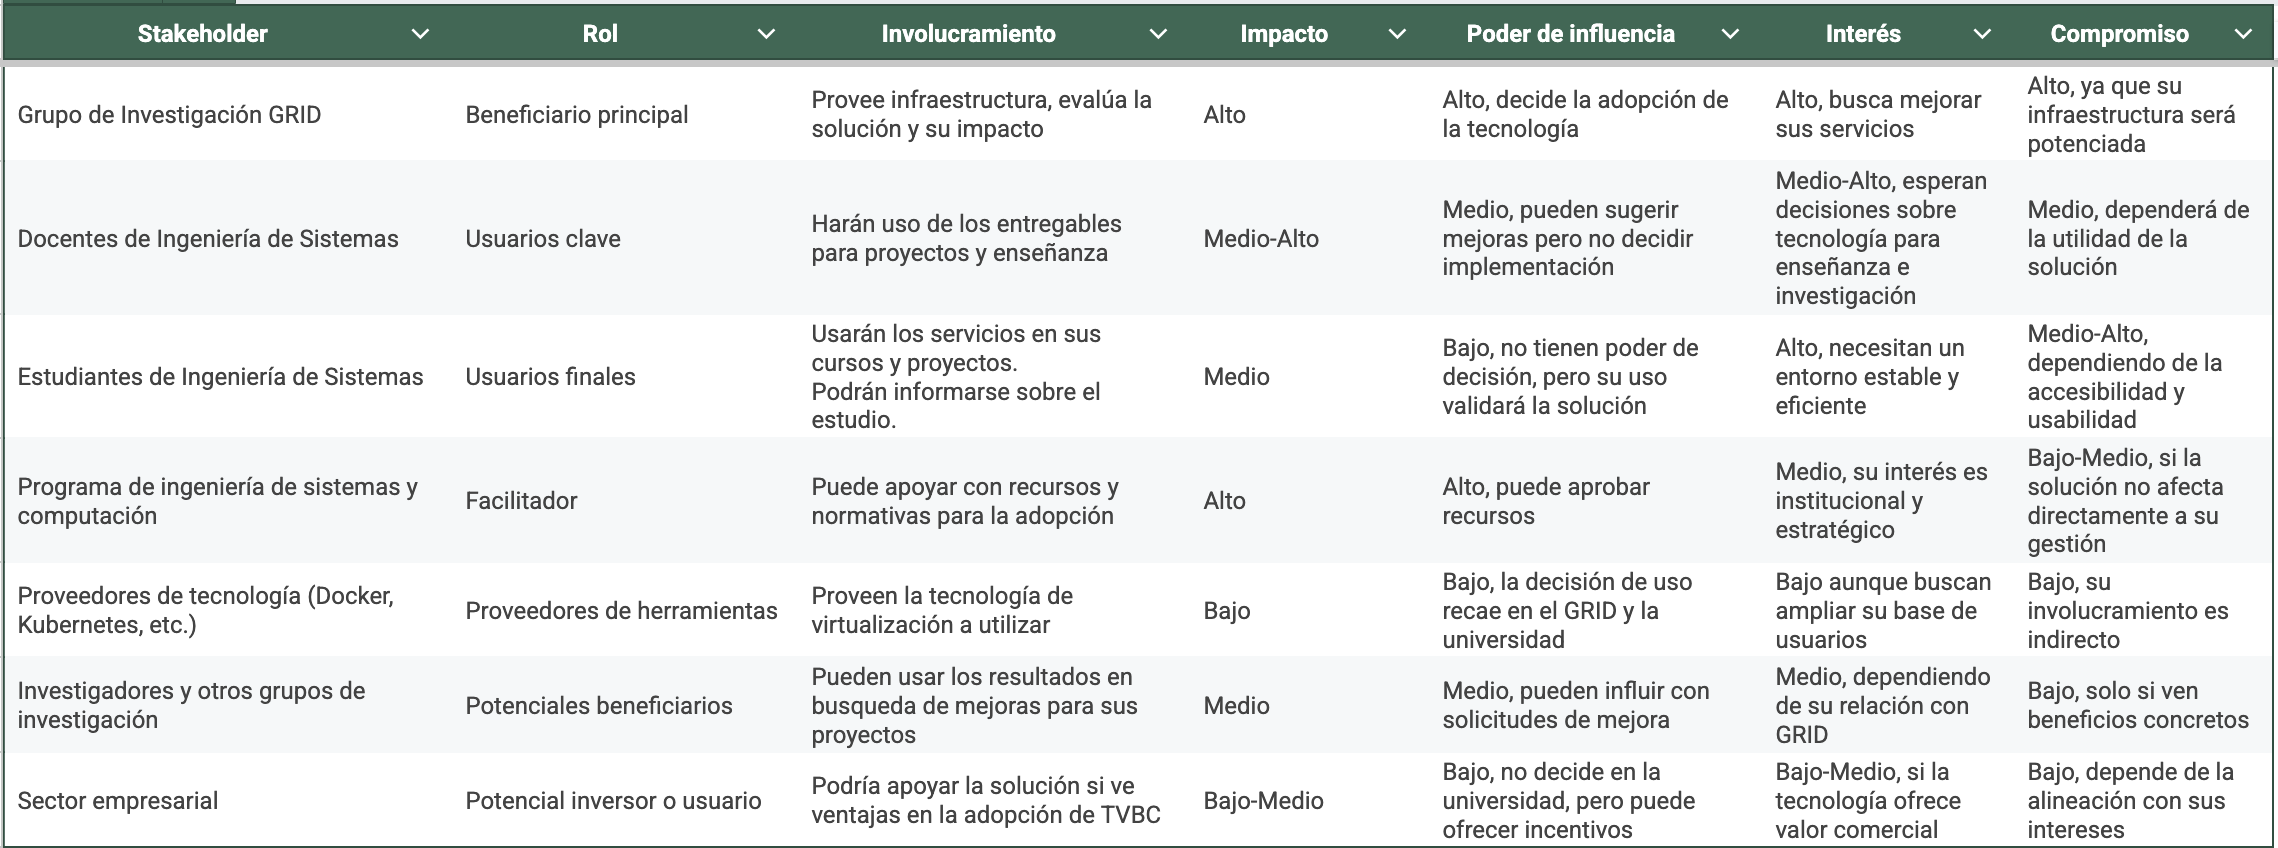
\includegraphics[width=\textwidth]{tablas-images/cp1/definicionStakeholders.png}
    \caption{Análisis de stakeholders del proyecto}
    \label{tab:tabla-stakeholders}
\end{table}

\section*{1.2 Priorización de stakeholders}
\addcontentsline{toc}{section}{Priorización de stakeholders}
A partir del análisis de stakeholders, se priorizaron aquellos que tienen mayor impacto y poder de influencia en el proyecto. Esta priorización permite enfocar los esfuerzos de comunicación y gestión de expectativas hacia
los stakeholders más relevantes, asegurando que sus necesidades sean atendidas de manera especial.

\begin{figure}[H]
    \centering
    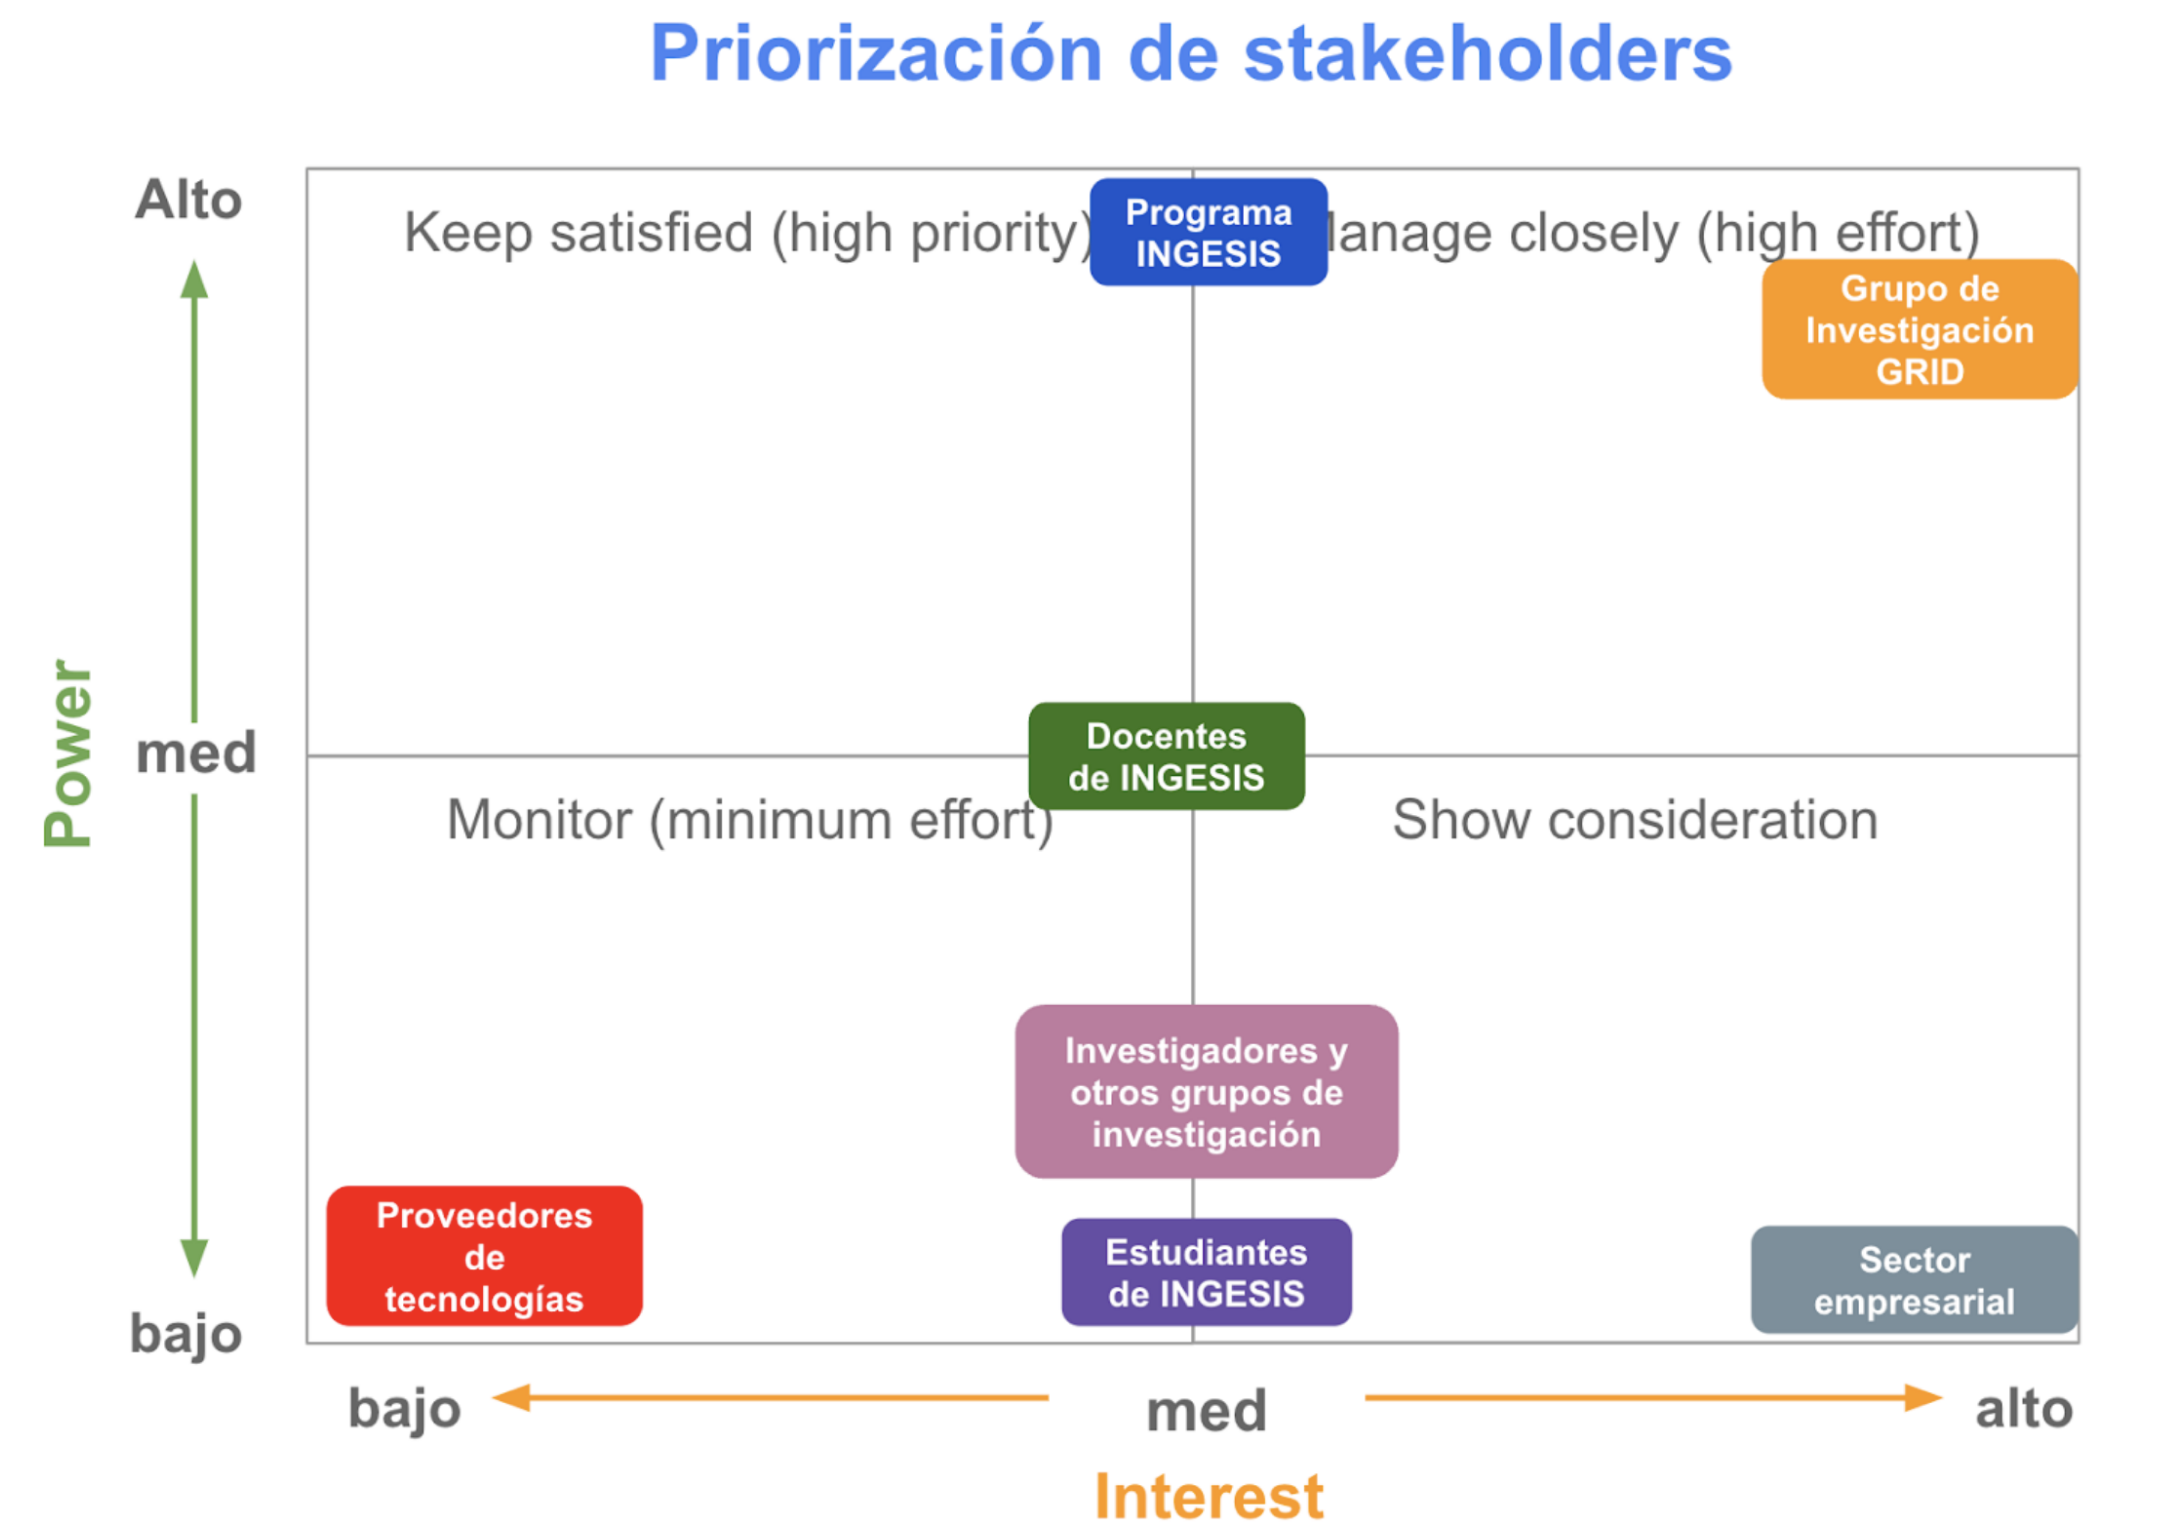
\includegraphics[width=\textwidth] {tablas-images/cp1/priorizacionStakeholders.png}
    \caption{Priorización de stakeholders del proyecto}\label{fig:tabla-priorizacion-stakeholders}
\end{figure}

\section*{1.3 Integrantes y áreas de trabajo del GRID}
\addcontentsline{toc}{section}{Integrantes y áreas de trabajo del GRID}
El GRID está compuesto por un equipo multidisciplinario de investigadores y profesionales, cada uno con áreas de especialización diferentes. A continuación se presentan los diferentes integrantes y sus respectivas áreas de trabajo:

\begin{itemize}
  \item \href{https://scienti.minciencias.gov.co/cvlac/visualizador/generarCurriculoCv.do?cod_rh=0000210897}{\textbf{Christian Andrés Candela Uribe}}: Microservicios, desarrollo de software, minería de datos, infraestructura TI
  \item \href{https://scienti.minciencias.gov.co/cvlac/visualizador/generarCurriculoCv.do?cod_rh=0001383939}{\textbf{Luis Eduardo Sepúlveda Rodríguez}}: Infraestructura de TI, HPC, computación paralela
  \item \href{https://scienti.minciencias.gov.co/cvlac/visualizador/generarCurriculoCv.do?cod_rh=0001638854}{\textbf{Carlos Andrés Flórez Villarraga}}: Programación y algoritmia, Activa, inteligencia artificial
  \item \href{https://scienti.minciencias.gov.co/cvlac/visualizador/generarCurriculoCv.do?cod_rh=0001343801}{\textbf{Carlos Eduardo Gómez Montoya}}: Networking, ingeniería de software, cloud computing
  \item \href{https://scienti.minciencias.gov.co/cvlac/visualizador/generarCurriculoCv.do?cod_rh=0001398775}{\textbf{Sergio Augusto Cardona Torres}}: Big data y análisis de datos, ingeniería de software, educación asistida por computador - sistemas adaptativos, informática educativa
  \item \href{https://scienti.minciencias.gov.co/cvlac/visualizador/generarCurriculoCv.do?cod_rh=0000193550}{\textbf{Sonia Jaramillo Valbuena}}: Big data, electroquímica, inteligencia artificial
  \item \href{https://scienti.minciencias.gov.co/cvlac/visualizador/generarCurriculoCv.do?cod_rh=0000283495}{\textbf{Julián Esteban Gutiérrez Posada}}: Microservicios, desarrollo de software, minería de datos, infraestructura TI, HPC, computación paralela, networking, ingeniería de software
\end{itemize}

\section*{1.4 Misión del GRID}
\addcontentsline{toc}{section}{Misión del GRID}

La misión del GRID es heredada de la Universidad del Quindío. A continuación se presenta la misión del GRID:

\begin{quote}
La Universidad del Quindío contribuye a la transformación de la sociedad, mediante la formación integral desde el ser, el saber y el hacer, de líderes reflexivos y gestores del cambio; con estándares de calidad, a través de una oferta de formación en diferentes metodologías, que responda a una sociedad basada en el conocimiento; una investigación pertinente, que aporte a la solución de las problemáticas del desarrollo e integrada con la extensión y proyección social; educando en tiempos del posconflicto y de la consolidación de la paz, apoyada en una gestión creativa y con estándares de calidad.
\end{quote}

A partir de esta misión, se identifican los siguientes pilares fundamentales:

\begin{itemize}
    \item \textbf{Docencia:} La Universidad del Quindío contribuye a la transformación de la sociedad, mediante la formación integral desde el ser, el saber y el hacer, de líderes reflexivos y gestores del cambio; con estándares de calidad, a través de una oferta de formación en diferentes metodologías, que responda a una sociedad basada en el conocimiento.

    \item \textbf{Investigación:} Una investigación pertinente, que aporte a la solución de las problemáticas del desarrollo e integrada con la extensión y proyección social.

    \item \textbf{Extensión y Desarrollo Social:} Apoyada en una gestión creativa y con estándares de calidad.

    \item \textbf{Responsabilidad Social:} Educando en tiempos del posconflicto y de la consolidación de la paz.
\end{itemize}

\section*{1.5 Visión del GRID}
\addcontentsline{toc}{section}{Visión del GRID}

\begin{quote}
En el año 2025, la Universidad del Quindío estará consolidada como una institución \textit{Pertinente - Creativa - Integradora}, acreditada de alta calidad, con reconocimiento nacional e internacional en sus procesos de formación a través de diferentes metodologías, de investigación, extensión, proyección y responsabilidad social.
\end{quote}

A partir de esta visión, se destacan los siguientes enfoques estratégicos:

\begin{itemize}
    \item \textbf{Gestión:} La Universidad del Quindío estará consolidada como una institución \textit{Pertinente --- Creativa --- Integradora}.

    \item \textbf{Docencia:} Acreditada de alta calidad en sus procesos de formación a través de diferentes metodologías.

    \item \textbf{Investigación:} Consolidada como pertinente y de alta calidad en sus procesos de investigación.

    \item \textbf{Extensión y Desarrollo Social:} Procesos creativos e integradores en proyección social.

    \item \textbf{Responsabilidad Social:} Reconocimientos en sus procesos de responsabilidad social.
\end{itemize}

\section*{1.6 Impacto del proyecto en el GRID}
\addcontentsline{toc}{section}{Impacto del proyecto en el GRID}

El proyecto tiene como objetivo apoyar los procesos de \textbf{docencia}, \textbf{investigación} 
y \textbf{extensión} mediante la especificación de una arquitectura de tecnologías de 
virtualización basada en contenedores (VBC). 

Este trabajo se enfoca en la identificación de una tecnología de contenerización que 
\textbf{agregue valor a los procesos del GRID}, beneficiando a \textbf{docentes}, \textbf{estudiantes} 
y cualquier parte interesada que participe en los proyectos y actividades desarrolladas 
por este grupo de investigación.

\section*{1.7 Caracterización de la infraestructura tecnológica del GRID}
\addcontentsline{toc}{section}{Caracterización de la infraestructura tecnológica del GRID}
En el siguiente formato se van a especificar las características técnicas de la infraestructura tecnológica del GRID disponible para temas de virtualización.\ \href{https://docs.google.com/spreadsheets/d/14NBv72ucVTrLqGIldYdIsjdBGt3QlgwcblcVRis-DaQ/edit?usp=sharing}{Macro de la ficha técnica}
% Archivo de caracterización de infraestructura corregido

% Torre HP 1
\begin{table}[H]
\centering
\caption{Ficha técnica --- Torre 1}\label{tab:torre-hp-1}
\begin{tabular}{|p{0.6\textwidth}|p{0.3\textwidth}|}
\hline
\multicolumn{2}{|l|}{\textbf{DESCRIPCIÓN FÍSICA:} Servidor tipo torre} \\ \hline
\textbf{TIPO DE RECURSO:} Torre &
\multirow{5}{*}{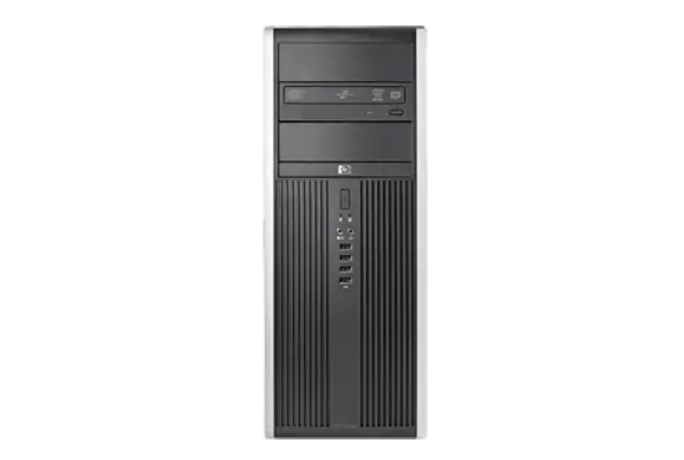
\includegraphics[width=0.25\textwidth,height=4cm,keepaspectratio]{tablas-images/cp1/torres/torre-1.png}} \\ \cline{1-1}
\textbf{MODELO:} Desconocido & \\ \cline{1-1}
\textbf{MARCA:} HP & \\ \cline{1-1}
\textbf{CÓDIGO DE INVENTARIO:} 7 24390 49867 3 & \\ \cline{1-1}
\textbf{NÚMERO EN CPD:} 14 & \\ \hline
\multicolumn{2}{|l|}{\textbf{ESPECIFICACIONES TÉCNICAS}} \\ \hline
\multicolumn{2}{|p{0.95\textwidth}|}{
\footnotesize
- 8 entradas USB (4 al frente, 4 en la parte trasera)
- Entrada de audio y microfono
- Entrada HDMI
- Lector de DVDs
- 3 puertos Ethernet (Parte trasera)
- Entrada Displayport
- Puertos PS/2 (Teclado y Ratón)
} \\ \hline
\multicolumn{2}{|l|}{\textbf{PROPÓSITO:} Hipervisor de XCP-ng} \\ \hline
\multicolumn{2}{|l|}{\textbf{OPORTUNIDAD DE USO:} Proyectos del \GRID} \\ \hline
\multicolumn{2}{|p{0.9\textwidth}|}{\textbf{OBSERVACIONES:} El Equipo no tiene modelo. El equipo está diseñado para usuario final pero fue adaptado para entornos de virtualización.} \\ \hline
\end{tabular}
\end{table}


% Torre 2
\begin{table}[H]
\centering
\caption{Ficha técnica --- Torre 2}\label{tab:torre-2}
\begin{tabular}{|p{0.6\textwidth}|p{0.3\textwidth}|}
\hline
\multicolumn{2}{|l|}{\textbf{DESCRIPCIÓN FÍSICA:} Servidor tipo torre} \\ \hline
\textbf{TIPO DE RECURSO:} Torre & 
\multirow{5}{*}{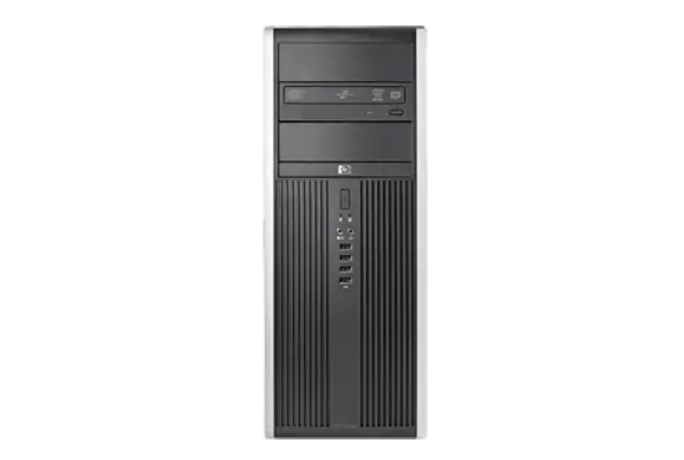
\includegraphics[width=0.25\textwidth,height=4cm,keepaspectratio]{tablas-images/cp1/torres/torre-1.png}} \\ \cline{1-1}
\textbf{MODELO:} Desconocido & \\ \cline{1-1}
\textbf{MARCA:} HP & \\ \cline{1-1}
\textbf{CÓDIGO DE INVENTARIO:} 7 24390 49861 1 & \\ \cline{1-1}
\textbf{NÚMERO EN CPD:} 12 & \\ \hline
\multicolumn{2}{|l|}{\textbf{ESPECIFICACIONES TÉCNICAS}} \\ \hline
\multicolumn{2}{|p{0.95\textwidth}|}{
\footnotesize
- 8 entradas USB (4 al frente, 4 en la parte trasera)
- Entrada de audio y microfono
- Entrada HDMI
- Lector de DVDs
- 3 puertos Ethernet (Parte trasera)
- Entrada Displayport
- Puertos PS/2 (Teclado y Ratón)
} \\ \hline
\multicolumn{2}{|l|}{\textbf{PROPÓSITO:} Hipervisor de XCP-ng} \\ \hline
\multicolumn{2}{|l|}{\textbf{OPORTUNIDAD DE USO:} Proyectos del \GRID} \\ \hline
\multicolumn{2}{|p{0.9\textwidth}|}{\textbf{OBSERVACIONES:} El Equipo no tiene modelo. El equipo está diseñado para usuario final pero fue adaptado para entornos de virtualización.} \\ \hline
\end{tabular}
\end{table}

% Torre 3
\begin{table}[H]
\centering
\caption{Ficha técnica -- Torre 3}
\label{tab:torre-3}
\begin{tabular}{|p{0.6\textwidth}|p{0.3\textwidth}|}
\hline
\multicolumn{2}{|l|}{\textbf{DESCRIPCIÓN FÍSICA:} Servidor tipo torre} \\ \hline
\textbf{TIPO DE RECURSO:} Torre & 
\multirow{5}{*}{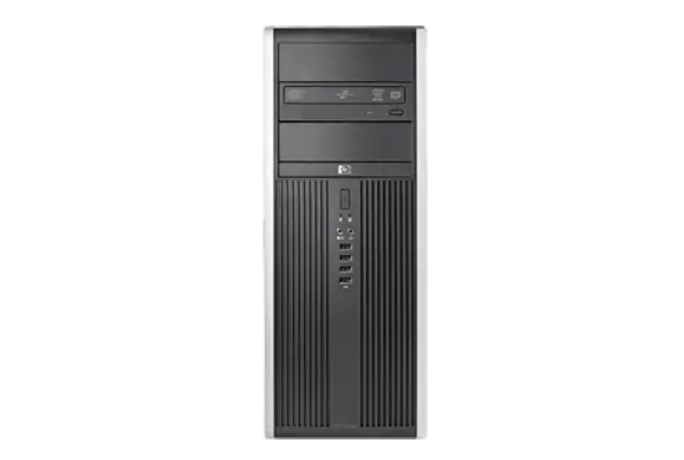
\includegraphics[width=0.25\textwidth,height=4cm,keepaspectratio]{tablas-images/cp1/torres/torre-1.png}} \\ \cline{1-1}
\textbf{MODELO:} Desconocido & \\ \cline{1-1}
\textbf{MARCA:} HP & \\ \cline{1-1}
\textbf{CÓDIGO DE INVENTARIO:} 7 24390 49969 4 & \\ \cline{1-1}
\textbf{NÚMERO EN CPD:} 13 & \\ \hline
\multicolumn{2}{|l|}{\textbf{ESPECIFICACIONES TÉCNICAS}} \\ \hline
\multicolumn{2}{|p{0.95\textwidth}|}{
\footnotesize
- 8 entradas USB (4 al frente, 4 en la parte trasera)
- Entrada de audio y microfono
- Entrada HDMI
- Lector de DVDs
- 3 puertos Ethernet (Parte trasera)
- Entrada Displayport
- Puertos PS/2 (Teclado y Ratón)
} \\ \hline
\multicolumn{2}{|l|}{\textbf{PROPÓSITO:} Hipervisor de XCP-ng} \\ \hline
\multicolumn{2}{|l|}{\textbf{OPORTUNIDAD DE USO:} Proyectos del \GRID} \\ \hline
\multicolumn{2}{|p{0.9\textwidth}|}{\textbf{OBSERVACIONES:} El Equipo no tiene modelo. El equipo está diseñado para usuario final pero fue adaptado para entornos de virtualización.} \\ \hline
\end{tabular}
\end{table}

% Torre 4
\begin{table}[H]
\centering
\caption{Ficha técnica --- Torre 4}
\label{tab:torre-4}
\begin{tabular}{|p{0.6\textwidth}|p{0.3\textwidth}|}
\hline
\multicolumn{2}{|l|}{\textbf{DESCRIPCIÓN FÍSICA:} Servidor tipo torre} \\ \hline
\textbf{TIPO DE RECURSO:} Torre & 
\multirow{5}{*}{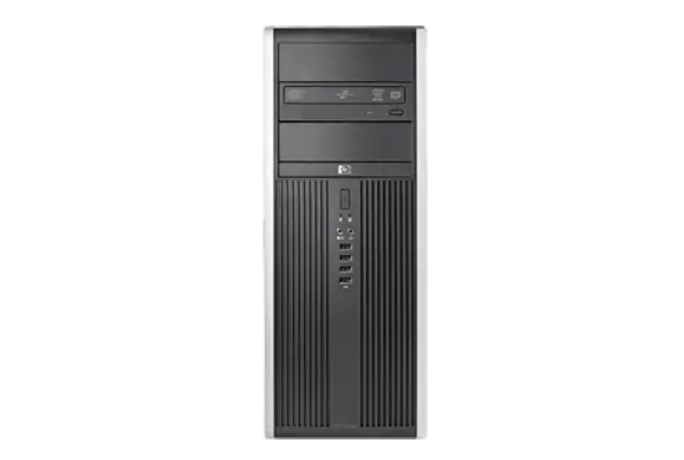
\includegraphics[width=0.25\textwidth,height=4cm,keepaspectratio]{tablas-images/cp1/torres/torre-1.png}} \\ \cline{1-1}
\textbf{MODELO:} Desconocido & \\ \cline{1-1}
\textbf{MARCA:} HP & \\ \cline{1-1}
\textbf{CÓDIGO DE INVENTARIO:} 7 24390 49879 4 & \\ \cline{1-1}
\textbf{NÚMERO EN CPD:} 14 & \\ \hline
\multicolumn{2}{|l|}{\textbf{ESPECIFICACIONES TÉCNICAS}} \\ \hline
\multicolumn{2}{|p{0.95\textwidth}|}{
\footnotesize
- 8 entradas USB (4 al frente, 4 en la parte trasera)
- Entrada de audio y microfono
- Entrada HDMI
- Lector de DVDs
- 3 puertos Ethernet (Parte trasera)
- Entrada Displayport
- Puertos PS/2 (Teclado y Ratón)
} \\ \hline
\multicolumn{2}{|l|}{\textbf{PROPÓSITO:} Hipervisor de XCP-ng} \\ \hline
\multicolumn{2}{|l|}{\textbf{OPORTUNIDAD DE USO:} Proyectos del \GRID} \\ \hline
\multicolumn{2}{|p{0.9\textwidth}|}{\textbf{OBSERVACIONES:} El Equipo no tiene modelo. El equipo está diseñado para usuario final pero fue adaptado para entornos de virtualización.} \\ \hline
\end{tabular}
\end{table}

% Torre 5
\begin{table}[H]
\centering
\caption{Ficha técnica --- Torre 5}
\label{tab:torre-5}
\begin{tabular}{|p{0.6\textwidth}|p{0.3\textwidth}|}
\hline
\multicolumn{2}{|l|}{\textbf{DESCRIPCIÓN FÍSICA:} Servidor tipo torre} \\ \hline
\textbf{TIPO DE RECURSO:} Torre & 
\multirow{5}{*}{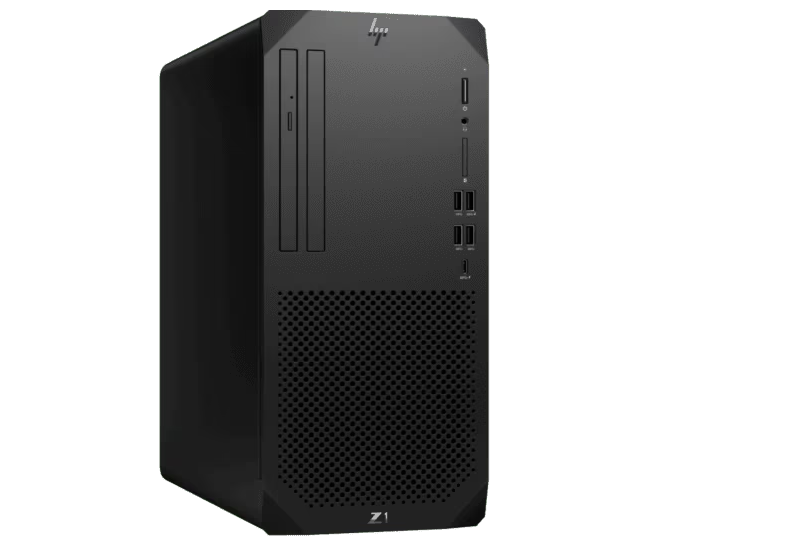
\includegraphics[width=0.25\textwidth,height=4cm,keepaspectratio]{tablas-images/cp1/torres/torre-2.png}} \\ \cline{1-1}
\textbf{MODELO:} G9 & \\ \cline{1-1}
\textbf{MARCA:} HP & \\ \cline{1-1}
\textbf{CÓDIGO DE INVENTARIO:} 72992 & \\ \cline{1-1}
\textbf{NÚMERO EN CPD:} 22 & \\ \hline
\multicolumn{2}{|l|}{\textbf{ESPECIFICACIONES TÉCNICAS}} \\ \hline
\multicolumn{2}{|p{0.95\textwidth}|}{
\footnotesize
- 9 entradas USB (4 al frente, 5 en la parte trasera)
- Entrada de audio y microfono
- Entrada HDMI
- Lector de DVDs
- 1 puerto Ethernet (Parte trasera)
- 2 Entrada Displayport
- Procesador Intel vPro i9
} \\ \hline
\multicolumn{2}{|l|}{\textbf{PROPÓSITO:} Hipervisor de XCP-ng} \\ \hline
\multicolumn{2}{|l|}{\textbf{OPORTUNIDAD DE USO:} Proyectos del \GRID} \\ \hline
\multicolumn{2}{|p{0.9\textwidth}|}{\textbf{OBSERVACIONES:} El equipo está diseñado para usuario final pero fue adaptado para entornos de virtualización.} \\ \hline
\end{tabular}
\end{table}

% Torre 6
\begin{table}[H]
\centering
\caption{Ficha técnica --- Torre 6}
\label{tab:torre-6}
\begin{tabular}{|p{0.6\textwidth}|p{0.3\textwidth}|}
\hline
\multicolumn{2}{|l|}{\textbf{DESCRIPCIÓN FÍSICA:} Servidor tipo torre} \\ \hline
\textbf{TIPO DE RECURSO:} Torre & 
\multirow{5}{*}{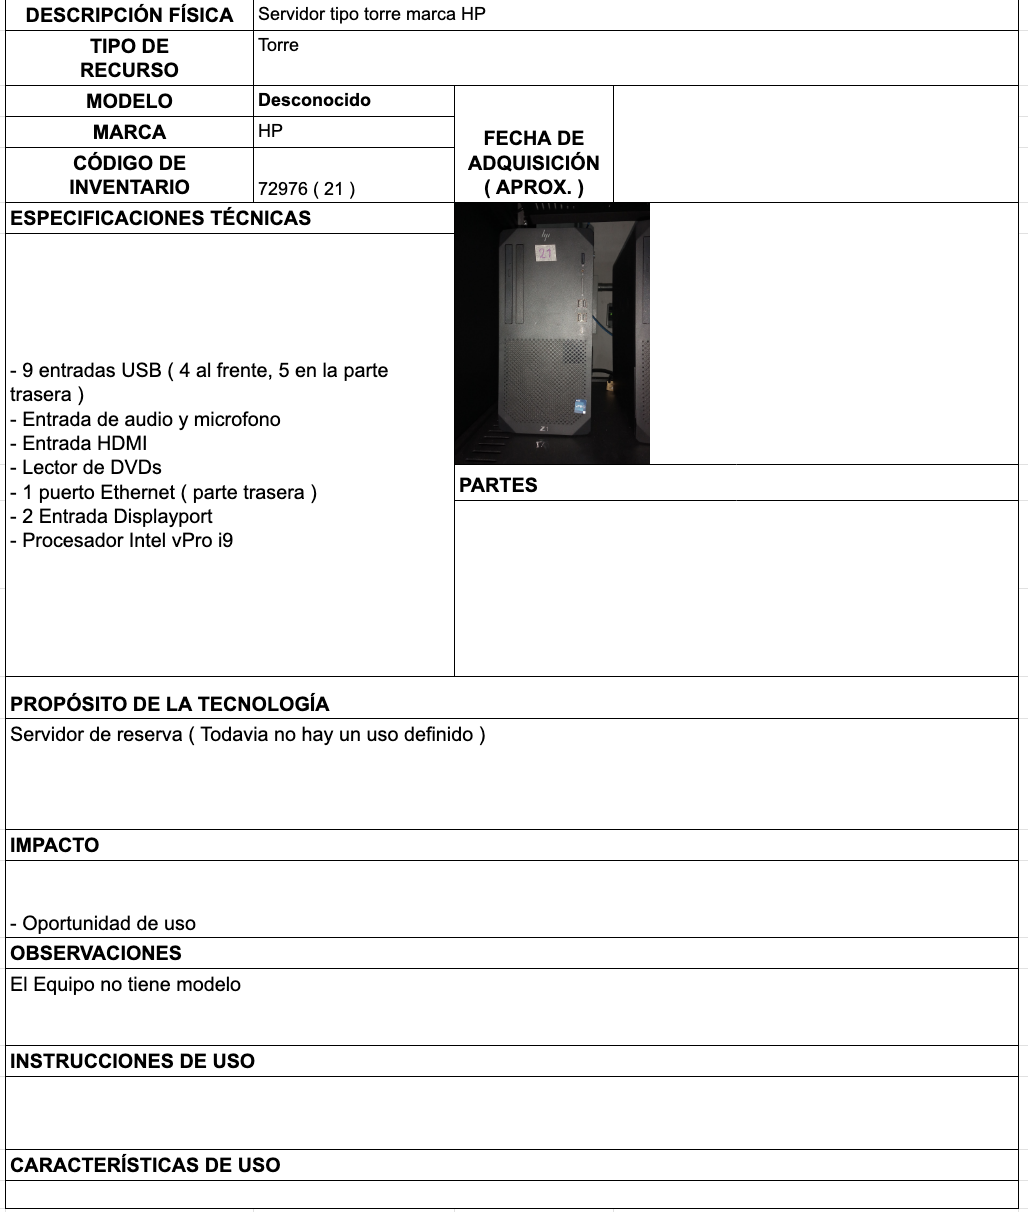
\includegraphics[width=0.25\textwidth,height=4cm,keepaspectratio]{tablas-images/cp1/torres/torre-6.png}} \\ \cline{1-1}
\textbf{MODELO:} Por definir & \\ \cline{1-1}
\textbf{MARCA:} Por definir & \\ \cline{1-1}
\textbf{CÓDIGO DE INVENTARIO:} Por definir & \\ \cline{1-1}
\textbf{FECHA DE ADQUISICIÓN (APROX.):} & \\ \hline
\multicolumn{2}{|l|}{\textbf{ESPECIFICACIONES TÉCNICAS}} \\ \hline
\multicolumn{2}{|p{0.95\textwidth}|}{
\footnotesize
Especificaciones por definir según imagen adjunta
} \\ \hline
\multicolumn{2}{|l|}{\textbf{PROPÓSITO:} Por definir} \\ \hline
\multicolumn{2}{|l|}{\textbf{IMPACTO:} Por evaluar} \\ \hline
\multicolumn{2}{|l|}{\textbf{OBSERVACIONES:} Ver imagen para detalles} \\ \hline
\end{tabular}
\end{table}

% Torre 7
\begin{table}[H]
\centering
\caption{Ficha técnica -- Torre 7}
\label{tab:torre-7}
\begin{tabular}{|p{0.6\textwidth}|p{0.3\textwidth}|}
\hline
\multicolumn{2}{|l|}{\textbf{DESCRIPCIÓN FÍSICA:} Servidor tipo torre} \\ \hline
\textbf{TIPO DE RECURSO:} Torre & 
\multirow{5}{*}{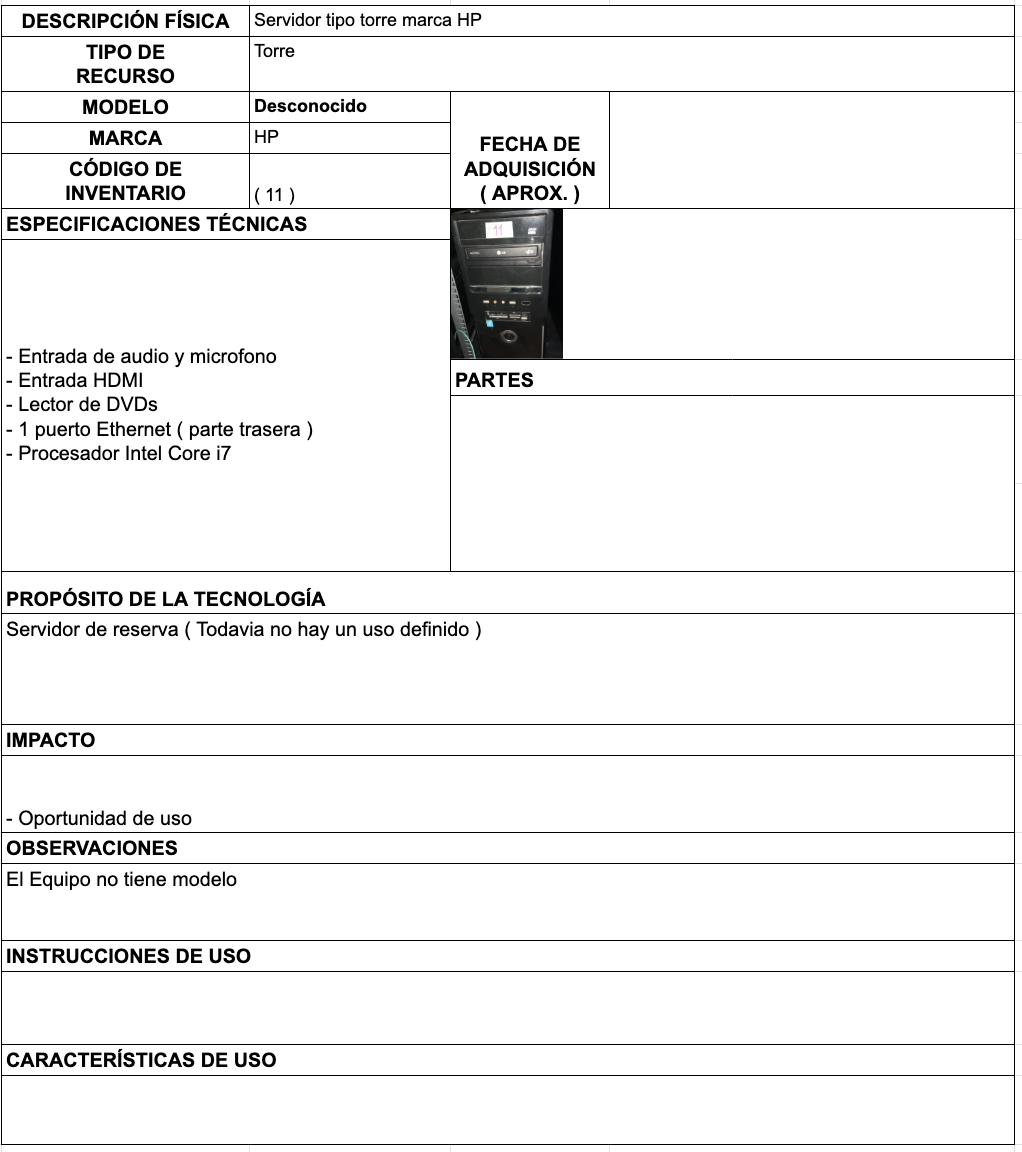
\includegraphics[width=0.25\textwidth,height=4cm,keepaspectratio]{tablas-images/cp1/torres/torre-7.png}} \\ \cline{1-1}
\textbf{MODELO:} Por definir & \\ \cline{1-1}
\textbf{MARCA:} Por definir & \\ \cline{1-1}
\textbf{CÓDIGO DE INVENTARIO:} Por definir & \\ \cline{1-1}
\textbf{FECHA DE ADQUISICIÓN (APROX.):} & \\ \hline
\multicolumn{2}{|l|}{\textbf{ESPECIFICACIONES TÉCNICAS}} \\ \hline
\multicolumn{2}{|p{0.95\textwidth}|}{
\footnotesize
Especificaciones por definir según imagen adjunta
} \\ \hline
\multicolumn{2}{|l|}{\textbf{PROPÓSITO:} Por definir} \\ \hline
\multicolumn{2}{|l|}{\textbf{IMPACTO:} Por evaluar} \\ \hline
\multicolumn{2}{|l|}{\textbf{OBSERVACIONES:} Ver imagen para detalles} \\ \hline
\end{tabular}
\end{table}

% Rack 1
\begin{table}[H]
\centering
\caption{Ficha técnica -- Rack 1}
\label{tab:rack-1}
\begin{tabular}{|p{0.6\textwidth}|p{0.3\textwidth}|}
\hline
\multicolumn{2}{|l|}{\textbf{DESCRIPCIÓN FÍSICA:} Servidor tipo rack} \\ \hline
\textbf{TIPO DE RECURSO:} Rack & 
\multirow{5}{*}{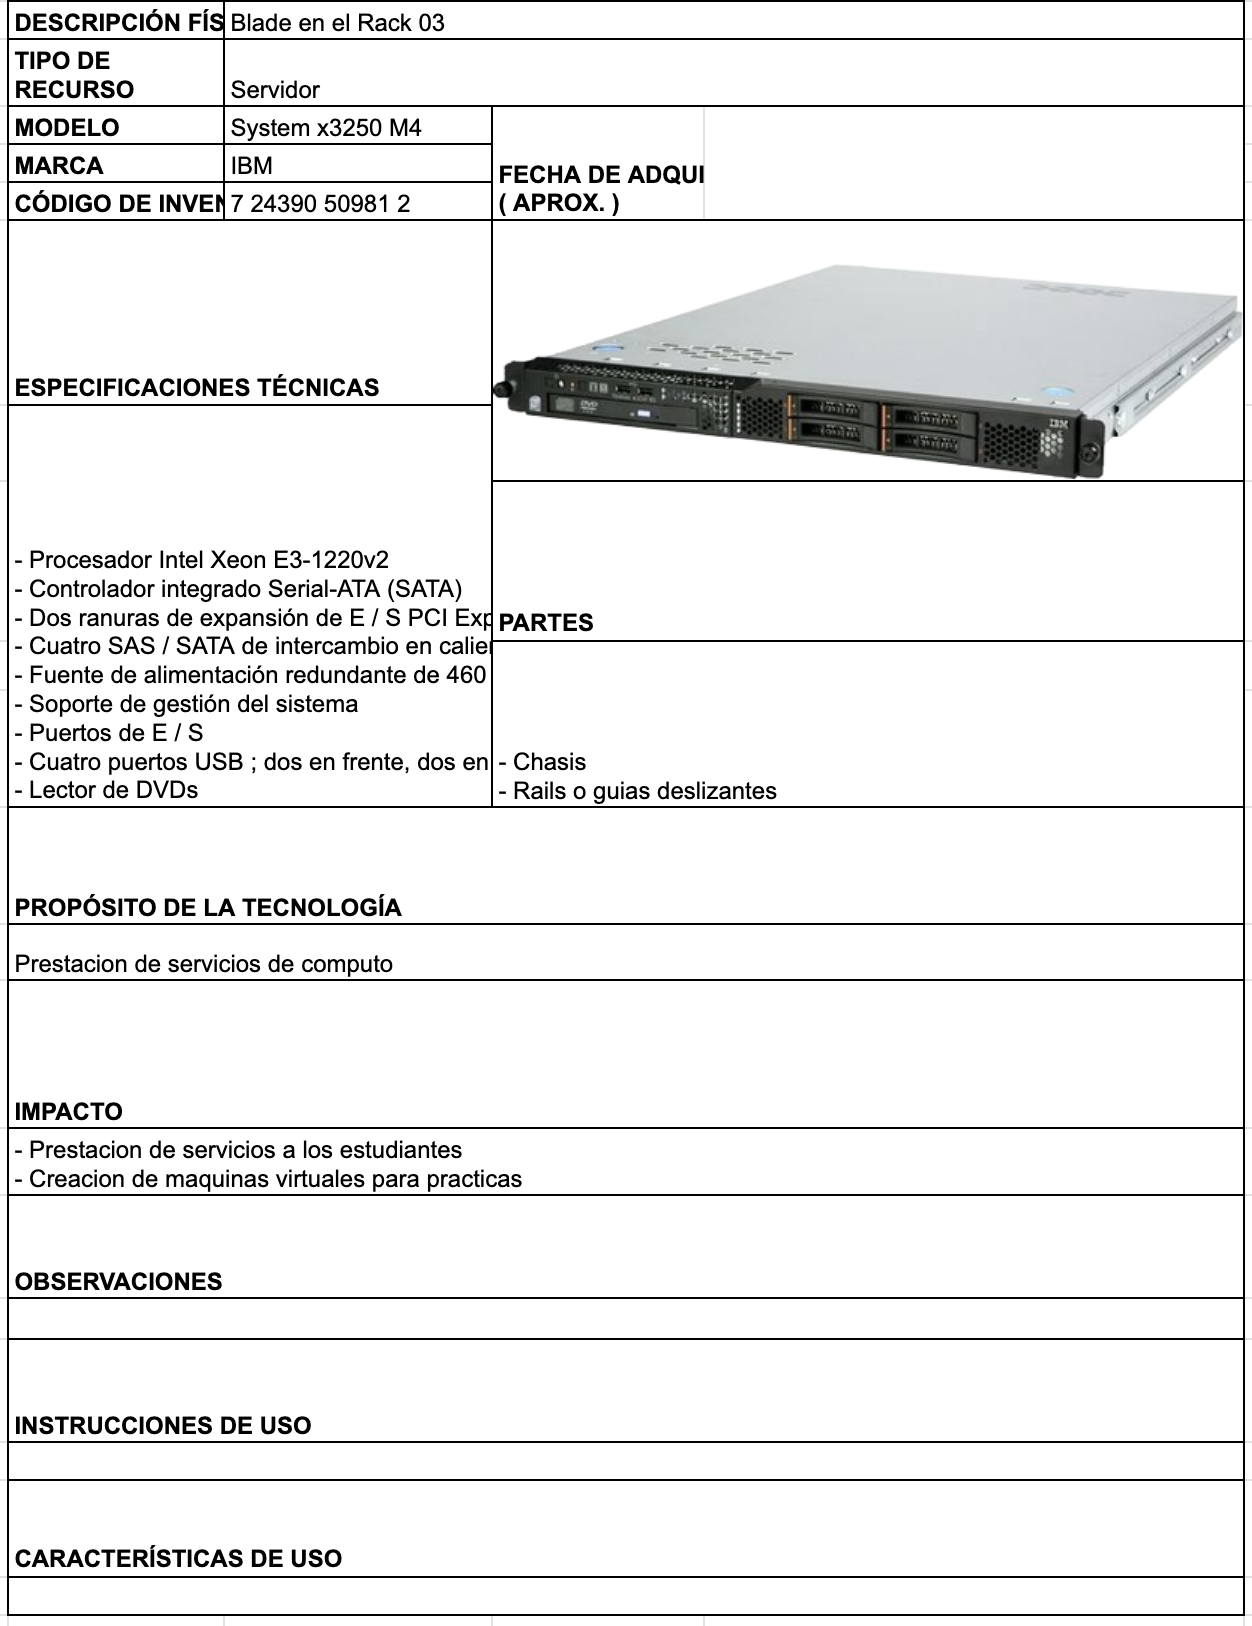
\includegraphics[width=0.25\textwidth,height=4cm,keepaspectratio]{tablas-images/cp1/racks/rack-1.png}} \\ \cline{1-1}
\textbf{MODELO:} Por definir & \\ \cline{1-1}
\textbf{MARCA:} Por definir & \\ \cline{1-1}
\textbf{CÓDIGO DE INVENTARIO:} Por definir & \\ \cline{1-1}
\textbf{FECHA DE ADQUISICIÓN (APROX.):} & \\ \hline
\multicolumn{2}{|l|}{\textbf{ESPECIFICACIONES TÉCNICAS}} \\ \hline
\multicolumn{2}{|p{0.95\textwidth}|}{
\footnotesize
Especificaciones por definir según imagen adjunta
} \\ \hline
\multicolumn{2}{|l|}{\textbf{PROPÓSITO:} Por definir} \\ \hline
\multicolumn{2}{|l|}{\textbf{IMPACTO:} Por evaluar} \\ \hline
\multicolumn{2}{|l|}{\textbf{OBSERVACIONES:} Ver imagen para detalles} \\ \hline
\end{tabular}
\end{table}

% Rack 2
\begin{table}[H]
\centering
\caption{Ficha técnica -- Rack 2}
\label{tab:rack-2}
\begin{tabular}{|p{0.6\textwidth}|p{0.3\textwidth}|}
\hline
\multicolumn{2}{|l|}{\textbf{DESCRIPCIÓN FÍSICA:} Servidor tipo rack} \\ \hline
\textbf{TIPO DE RECURSO:} Rack & 
\multirow{5}{*}{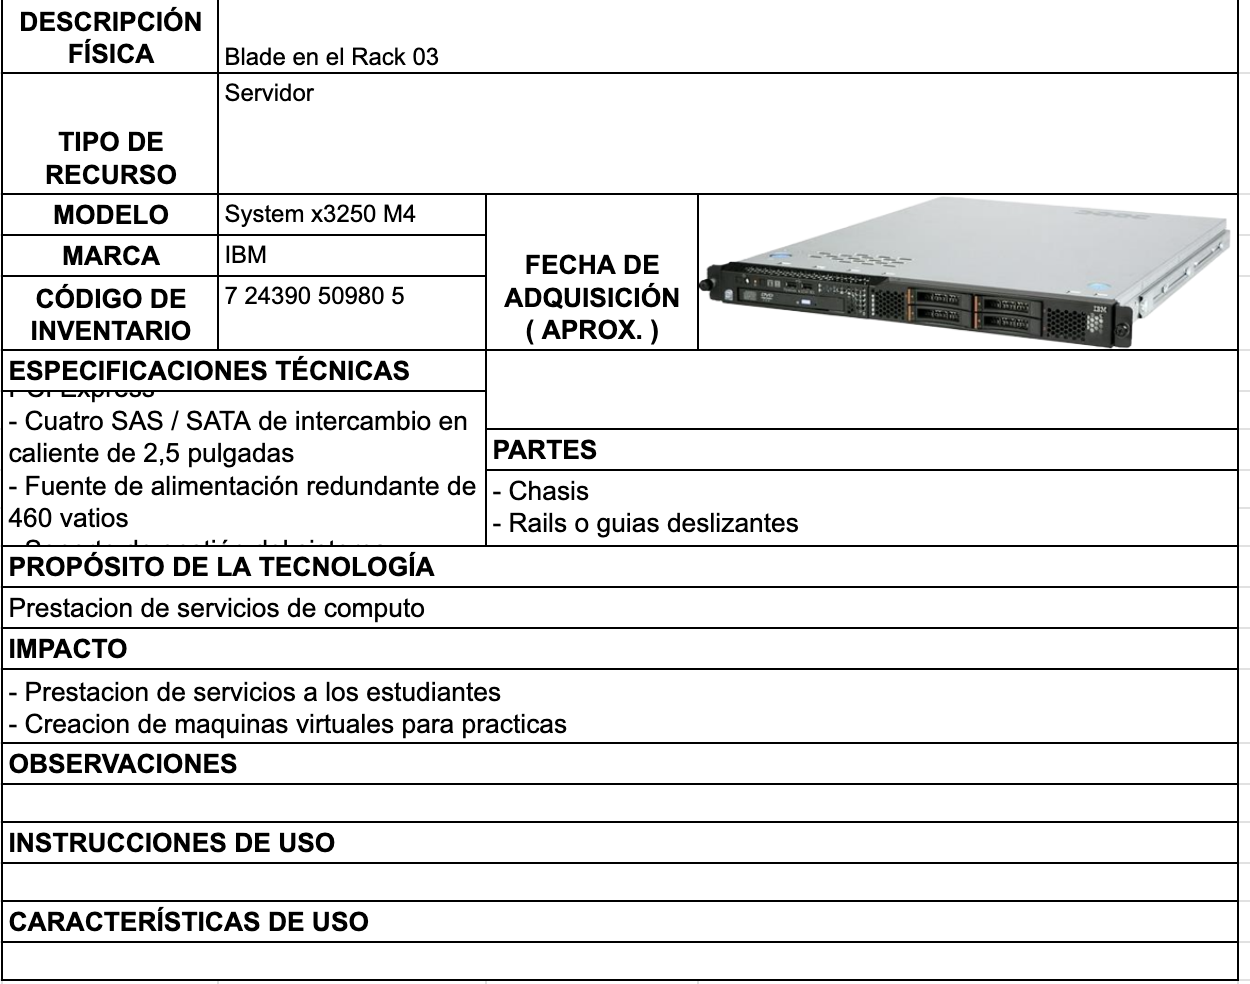
\includegraphics[width=0.25\textwidth,height=4cm,keepaspectratio]{tablas-images/cp1/racks/rack-2.png}} \\ \cline{1-1}
\textbf{MODELO:} Por definir & \\ \cline{1-1}
\textbf{MARCA:} Por definir & \\ \cline{1-1}
\textbf{CÓDIGO DE INVENTARIO:} Por definir & \\ \cline{1-1}
\textbf{FECHA DE ADQUISICIÓN (APROX.):} & \\ \hline
\multicolumn{2}{|l|}{\textbf{ESPECIFICACIONES TÉCNICAS}} \\ \hline
\multicolumn{2}{|p{0.95\textwidth}|}{
\footnotesize
Especificaciones por definir según imagen adjunta
} \\ \hline
\multicolumn{2}{|l|}{\textbf{PROPÓSITO:} Por definir} \\ \hline
\multicolumn{2}{|l|}{\textbf{IMPACTO:} Por evaluar} \\ \hline
\multicolumn{2}{|l|}{\textbf{OBSERVACIONES:} Ver imagen para detalles} \\ \hline
\end{tabular}
\end{table}

% Rack 3
\begin{table}[H]
\centering
\caption{Ficha técnica -- Rack 3}
\label{tab:rack-3}
\begin{tabular}{|p{0.6\textwidth}|p{0.3\textwidth}|}
\hline
\multicolumn{2}{|l|}{\textbf{DESCRIPCIÓN FÍSICA:} Servidor tipo rack} \\ \hline
\textbf{TIPO DE RECURSO:} Rack & 
\multirow{5}{*}{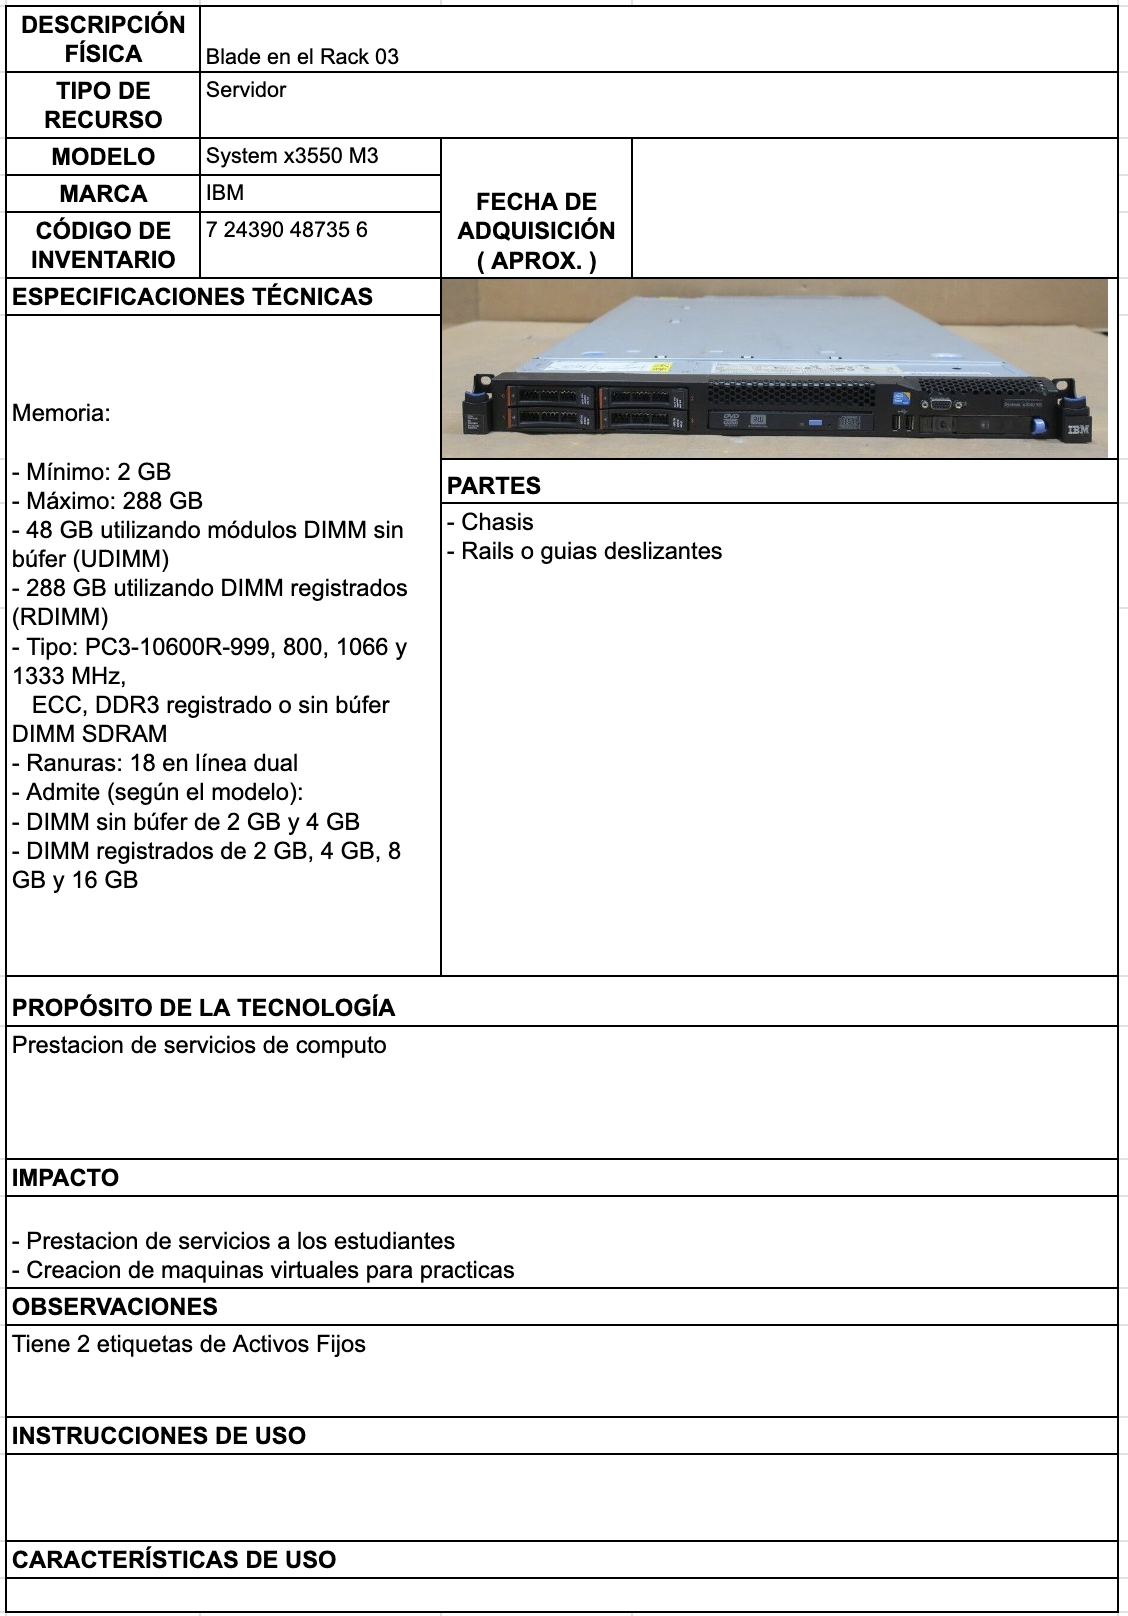
\includegraphics[width=0.25\textwidth,height=4cm,keepaspectratio]{tablas-images/cp1/racks/rack-3.png}} \\ \cline{1-1}
\textbf{MODELO:} Por definir & \\ \cline{1-1}
\textbf{MARCA:} Por definir & \\ \cline{1-1}
\textbf{CÓDIGO DE INVENTARIO:} Por definir & \\ \cline{1-1}
\textbf{FECHA DE ADQUISICIÓN (APROX.):} & \\ \hline
\multicolumn{2}{|l|}{\textbf{ESPECIFICACIONES TÉCNICAS}} \\ \hline
\multicolumn{2}{|p{0.95\textwidth}|}{
\footnotesize
Especificaciones por definir según imagen adjunta
} \\ \hline
\multicolumn{2}{|l|}{\textbf{PROPÓSITO:} Por definir} \\ \hline
\multicolumn{2}{|l|}{\textbf{IMPACTO:} Por evaluar} \\ \hline
\multicolumn{2}{|l|}{\textbf{OBSERVACIONES:} Ver imagen para detalles} \\ \hline
\end{tabular}
\end{table}

% Rack 4
\begin{table}[H]
\centering
\caption{Ficha técnica -- Rack 4}
\label{tab:rack-4}
\begin{tabular}{|p{0.6\textwidth}|p{0.3\textwidth}|}
\hline
\multicolumn{2}{|l|}{\textbf{DESCRIPCIÓN FÍSICA:} Servidor tipo rack} \\ \hline
\textbf{TIPO DE RECURSO:} Rack & 
\multirow{5}{*}{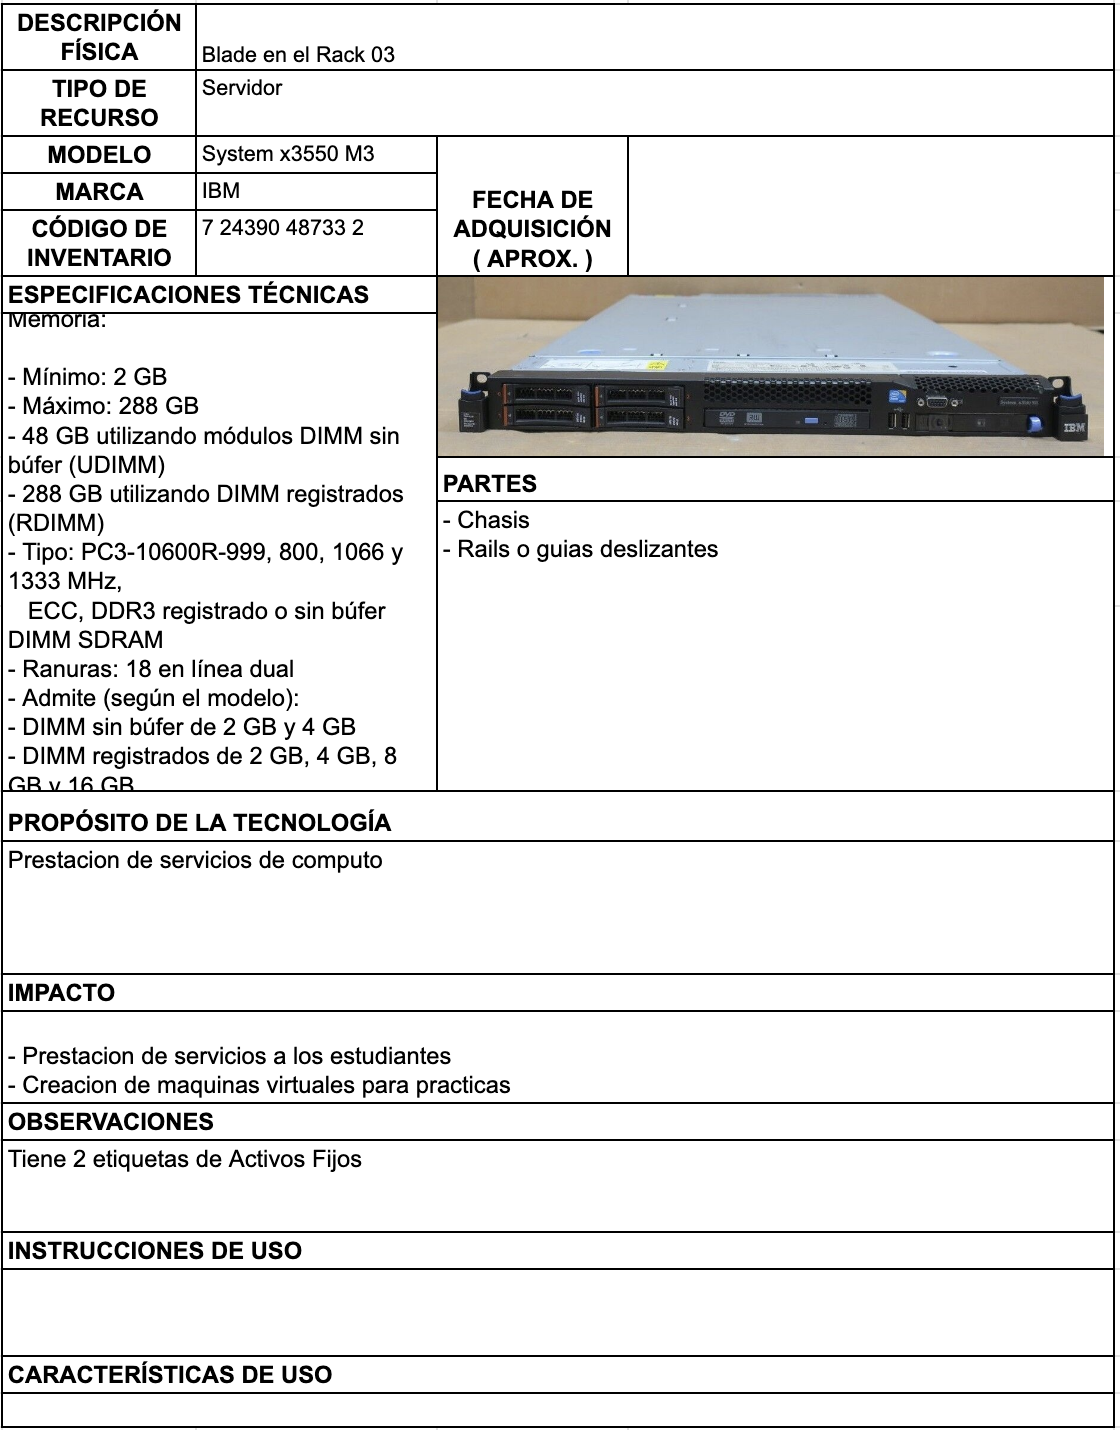
\includegraphics[width=0.25\textwidth,height=4cm,keepaspectratio]{tablas-images/cp1/racks/rack-4.png}} \\ \cline{1-1}
\textbf{MODELO:} Por definir & \\ \cline{1-1}
\textbf{MARCA:} Por definir & \\ \cline{1-1}
\textbf{CÓDIGO DE INVENTARIO:} Por definir & \\ \cline{1-1}
\textbf{FECHA DE ADQUISICIÓN (APROX.):} & \\ \hline
\multicolumn{2}{|l|}{\textbf{ESPECIFICACIONES TÉCNICAS}} \\ \hline
\multicolumn{2}{|p{0.95\textwidth}|}{
\footnotesize
Especificaciones por definir según imagen adjunta
} \\ \hline
\multicolumn{2}{|l|}{\textbf{PROPÓSITO:} Por definir} \\ \hline
\multicolumn{2}{|l|}{\textbf{IMPACTO:} Por evaluar} \\ \hline
\multicolumn{2}{|l|}{\textbf{OBSERVACIONES:} Ver imagen para detalles} \\ \hline
\end{tabular}
\end{table}

% Rack 5
\begin{table}[H]
\centering
\caption{Ficha técnica -- Rack 5}
\label{tab:rack-5}
\begin{tabular}{|p{0.6\textwidth}|p{0.3\textwidth}|}
\hline
\multicolumn{2}{|l|}{\textbf{DESCRIPCIÓN FÍSICA:} Servidor tipo rack} \\ \hline
\textbf{TIPO DE RECURSO:} Rack & 
\multirow{5}{*}{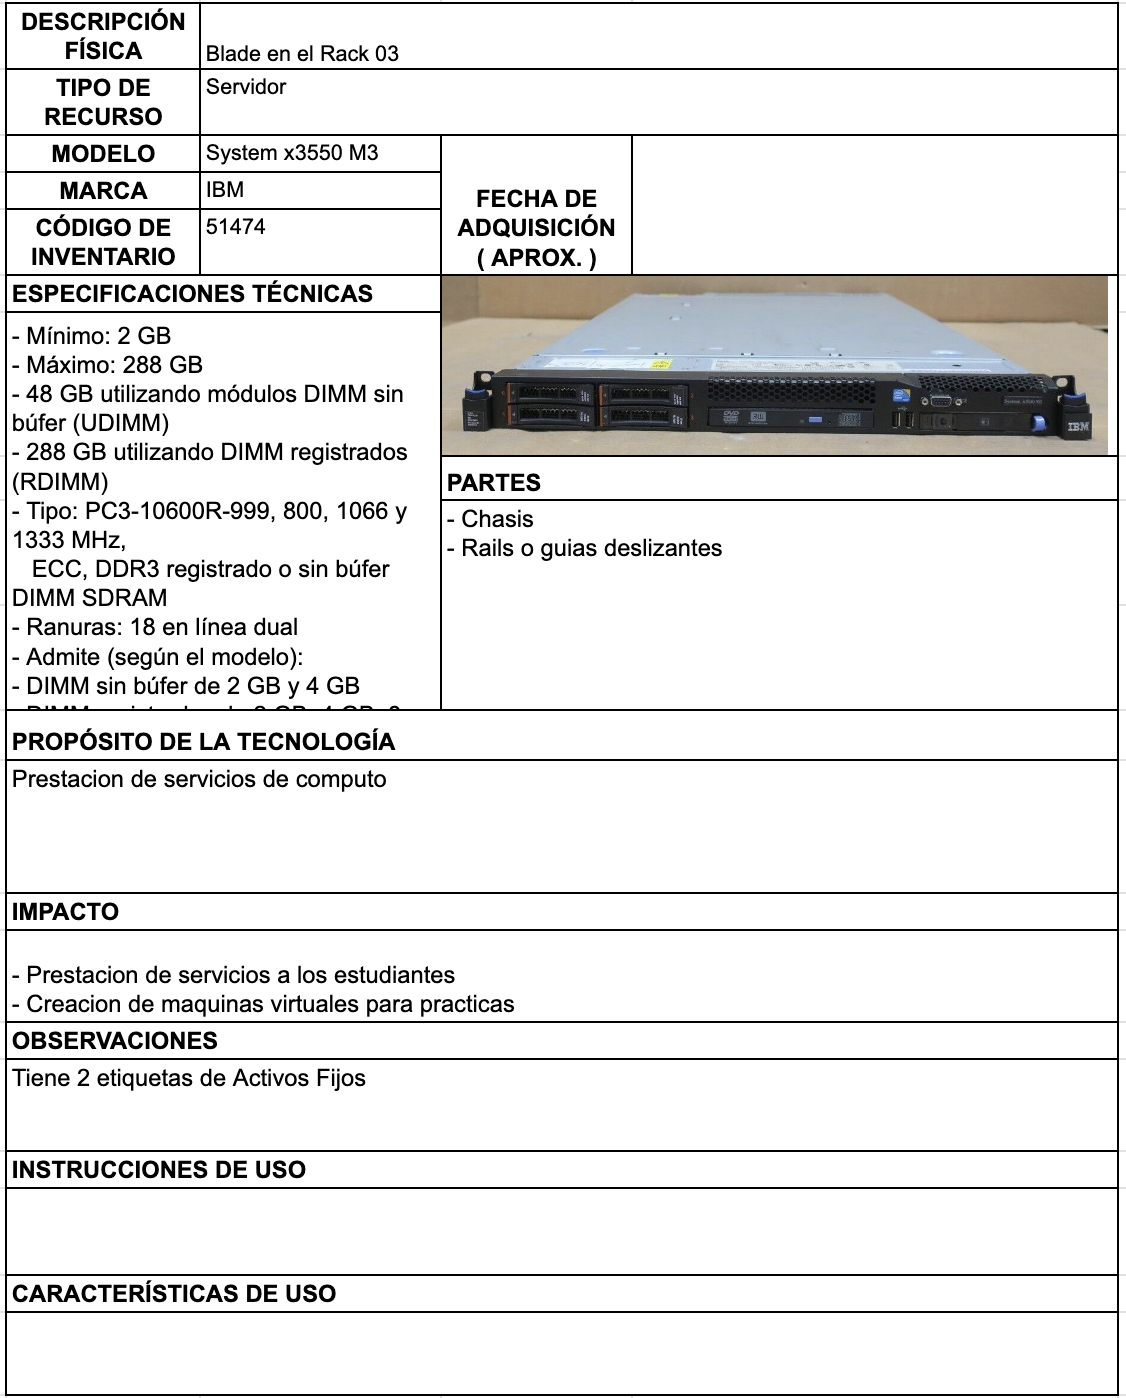
\includegraphics[width=0.25\textwidth,height=4cm,keepaspectratio]{tablas-images/cp1/racks/rack-5.png}} \\ \cline{1-1}
\textbf{MODELO:} Por definir & \\ \cline{1-1}
\textbf{MARCA:} Por definir & \\ \cline{1-1}
\textbf{CÓDIGO DE INVENTARIO:} Por definir & \\ \cline{1-1}
\textbf{FECHA DE ADQUISICIÓN (APROX.):} & \\ \hline
\multicolumn{2}{|l|}{\textbf{ESPECIFICACIONES TÉCNICAS}} \\ \hline
\multicolumn{2}{|p{0.95\textwidth}|}{
\footnotesize
Especificaciones por definir según imagen adjunta
} \\ \hline
\multicolumn{2}{|l|}{\textbf{PROPÓSITO:} Por definir} \\ \hline
\multicolumn{2}{|l|}{\textbf{IMPACTO:} Por evaluar} \\ \hline
\multicolumn{2}{|l|}{\textbf{OBSERVACIONES:} Ver imagen para detalles} \\ \hline
\end{tabular}
\end{table}

% NAS 1
\begin{table}[H]
\centering
\caption{Ficha técnica -- NAS 1}
\label{tab:nas-1}
\begin{tabular}{|p{0.6\textwidth}|p{0.3\textwidth}|}
\hline
\multicolumn{2}{|l|}{\textbf{DESCRIPCIÓN FÍSICA:} Sistema de almacenamiento conectado en red} \\ \hline
\textbf{TIPO DE RECURSO:} NAS (Network Attached Storage) & 
\multirow{5}{*}{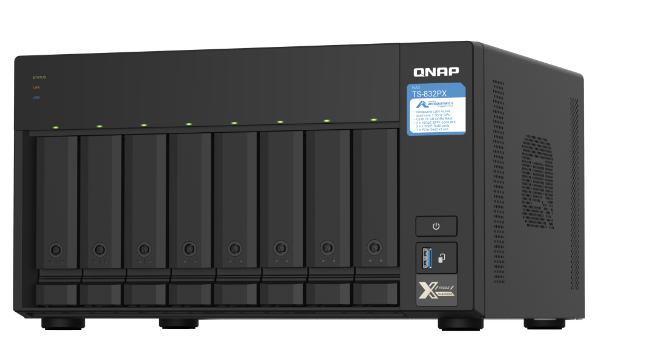
\includegraphics[width=0.25\textwidth,height=4cm,keepaspectratio]{tablas-images/cp1/NAS/nas-1.png}} \\ \cline{1-1}
\textbf{MODELO:} Por definir & \\ \cline{1-1}
\textbf{MARCA:} Por definir & \\ \cline{1-1}
\textbf{CÓDIGO DE INVENTARIO:} Por definir & \\ \cline{1-1}
\textbf{FECHA DE ADQUISICIÓN (APROX.):} & \\ \hline
\multicolumn{2}{|l|}{\textbf{ESPECIFICACIONES TÉCNICAS}} \\ \hline
\multicolumn{2}{|p{0.95\textwidth}|}{
\footnotesize
Especificaciones por definir según imagen adjunta
} \\ \hline
\multicolumn{2}{|l|}{\textbf{PROPÓSITO:} Por definir} \\ \hline
\multicolumn{2}{|l|}{\textbf{IMPACTO:} Por evaluar} \\ \hline
\multicolumn{2}{|l|}{\textbf{OBSERVACIONES:} Ver imagen para detalles} \\ \hline
\end{tabular}
\end{table}

% Firewall 1
\begin{table}[H]
\centering
\caption{Ficha técnica -- Firewall 1}
\label{tab:firewall-1}
\begin{tabular}{|p{0.6\textwidth}|p{0.3\textwidth}|}
\hline
\multicolumn{2}{|l|}{\textbf{DESCRIPCIÓN FÍSICA:} Sistema de seguridad de red} \\ \hline
\textbf{TIPO DE RECURSO:} Firewall & 
\multirow{5}{*}{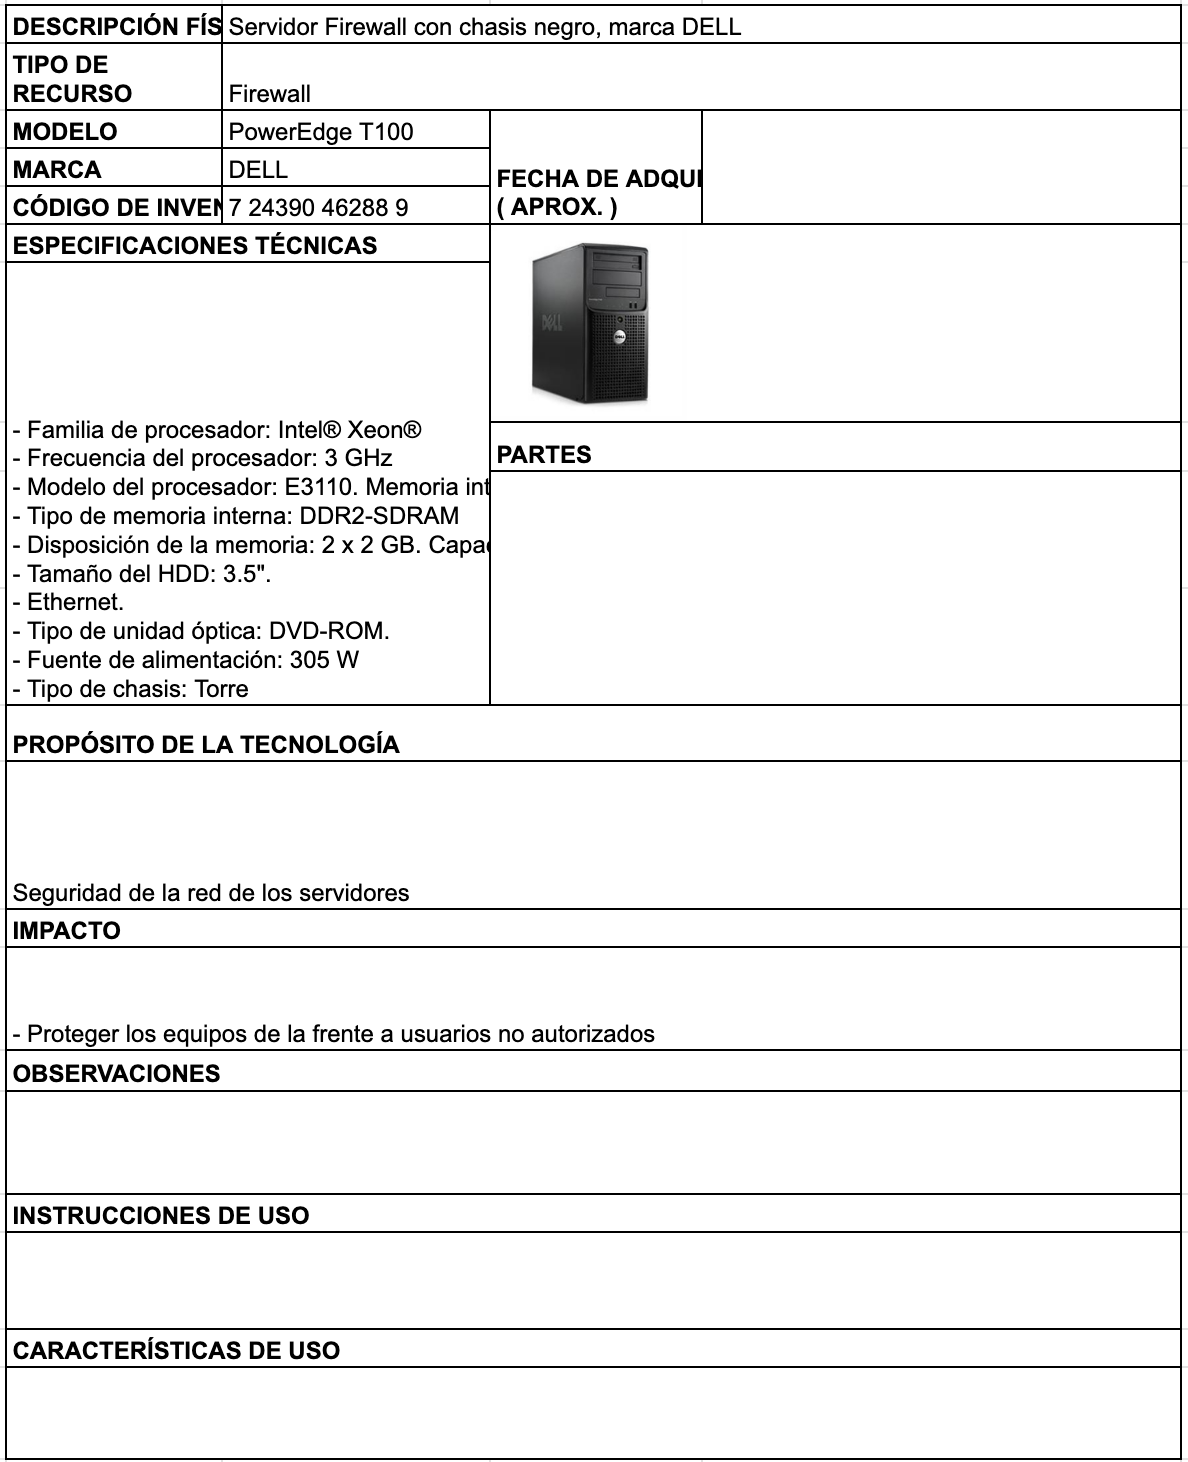
\includegraphics[width=0.25\textwidth,height=4cm,keepaspectratio]{tablas-images/cp1/firewall/firewall.png}} \\ \cline{1-1}
\textbf{MODELO:} Por definir & \\ \cline{1-1}
\textbf{MARCA:} Por definir & \\ \cline{1-1}
\textbf{CÓDIGO DE INVENTARIO:} Por definir & \\ \cline{1-1}
\textbf{FECHA DE ADQUISICIÓN (APROX.):} & \\ \hline
\multicolumn{2}{|l|}{\textbf{ESPECIFICACIONES TÉCNICAS}} \\ \hline
\multicolumn{2}{|p{0.95\textwidth}|}{
\footnotesize
Especificaciones por definir según imagen adjunta
} \\ \hline
\multicolumn{2}{|l|}{\textbf{PROPÓSITO:} Por definir} \\ \hline
\multicolumn{2}{|l|}{\textbf{IMPACTO:} Por evaluar} \\ \hline
\multicolumn{2}{|l|}{\textbf{OBSERVACIONES:} Ver imagen para detalles} \\ \hline
\end{tabular}
\end{table}

\section*{1.8 Caracterización de servicios del GRID}
\addcontentsline{toc}{section}{Caracterización de servicios del GRID}
El GRID ofrece una variedad de servicios tecnológicos a la comunidad académica, especialmente a los estudiantes de Ingeniería de Sistemas y Computación. Estos servicios incluyen:

\subsection*{1.8.1 Servicios actuales}
\addcontentsline{toc}{subsection}{Servicios actuales}
Los servicios actuales del GRID se centran en la provisión de infraestructura de TI, incluyendo máquinas virtuales, almacenamiento y redes. Estos servicios son utilizados principalmente por estudiantes y docentes

\begin{table}[H]
    \centering
    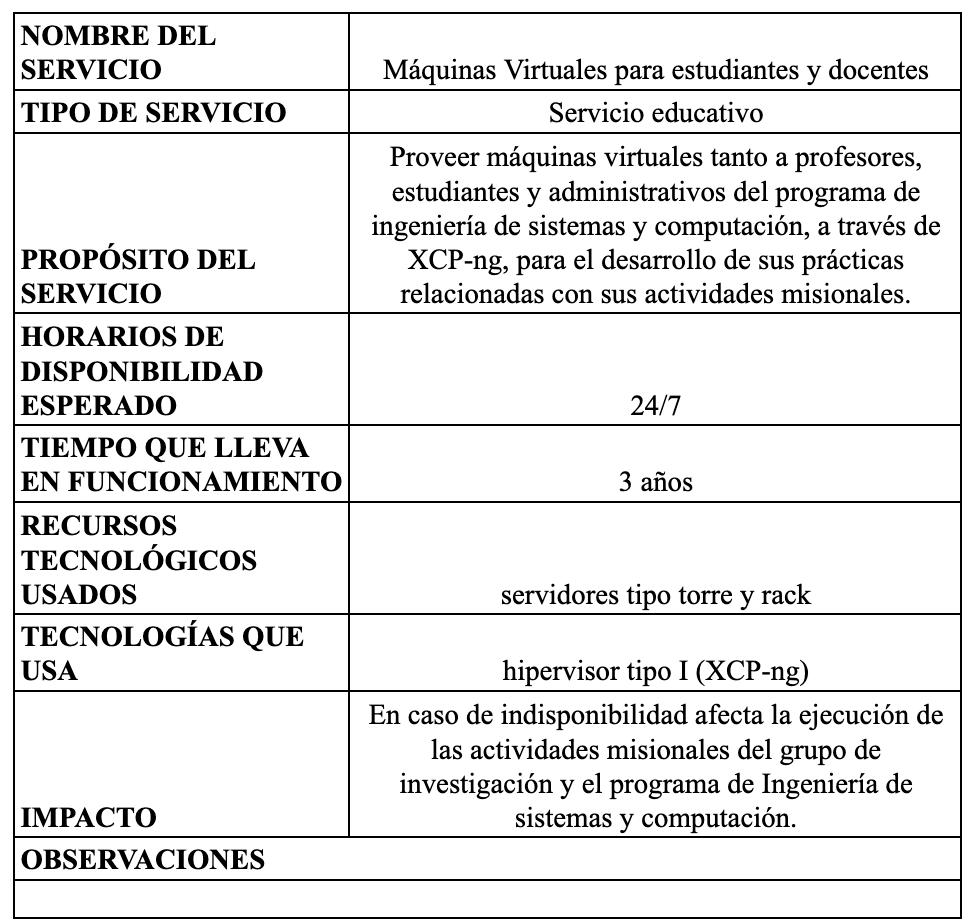
\includegraphics[width=\textwidth]{tablas-images/cp1/servicios-actuales/servicios-actuales.png}
    \caption{Caracterización de los servicios actuales del GRID}
    \label{tab:servicios-actuales}
\end{table}

\subsection*{1.8.2 Servicios esperados}
\addcontentsline{toc}{subsection}{Servicios esperados}
Los servicios esperados del GRID incluyen la implementación de tecnologías de virtualización basadas en contenedores (VBC) para mejorar la administración de la infraestructura de TI.

\begin{table}[H]
    \centering
    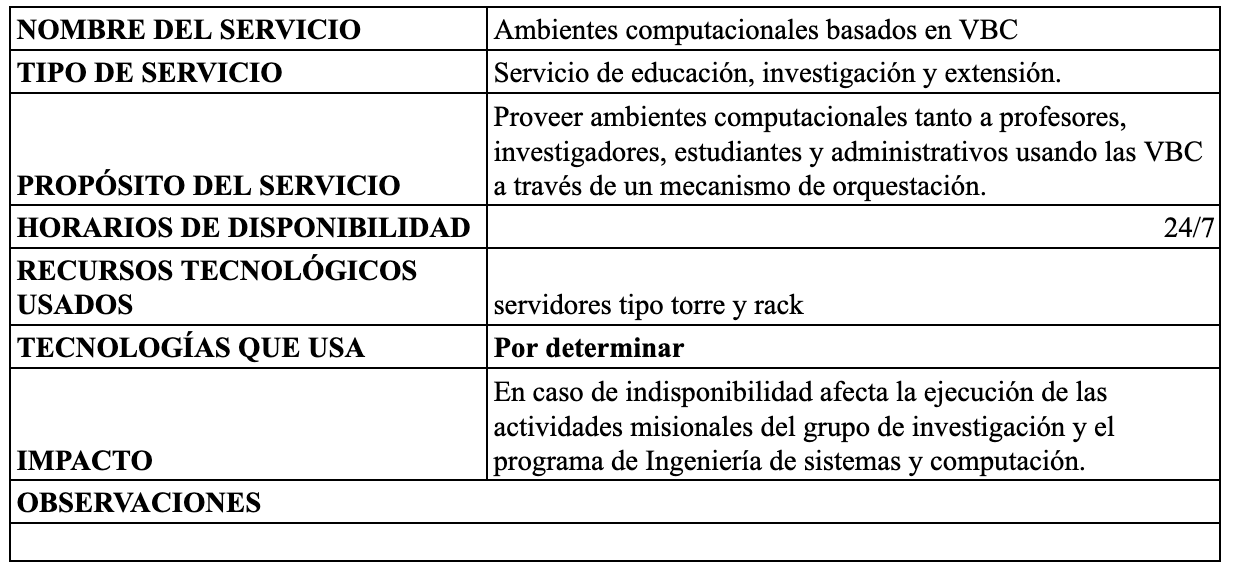
\includegraphics[width=\textwidth] {tablas-images/cp1/servicios-esperados/servicios-esperados.png}
    \caption{Caracterización de los servicios esperados del GRID}
    \label{tab:servicios-esperados}
\end{table}

\section*{1.9 Descripción de la oportunidad}
\addcontentsline{toc}{section}{Descripción de la oportunidad}

Actualmente el Grupo de Investigación en Redes, Información y Distribución (GRID) presenta diversas necesidades y oportunidades con relación a los servicios tecnológicos que ofrece a la Universidad del Quindío, en apoyo a sus objetivos misionales de docencia, investigación y extensión.

En este contexto, el GRID busca identificar tecnologías emergentes que permitan potenciar su capacidad de brindar servicios tecnológicos avanzados, tanto para su propio beneficio como para la comunidad académica dentro de su ámbito de influencia.

Con relación a lo anterior, las \textbf{tecnologías de virtualización basadas en procesos} se presentan como una alternativa para optimizar la gestión de recursos y servicios de tecnología informática (TI). Aunque el GRID cuenta con una infraestructura basada en máquinas virtuales, gestionadas mediante el hipervisor tipo I \textit{XCP-ng}, además de iniciativas de computación \textit{Desktop Cloud}, aún requiere de instancias computacionales más livianas para ampliar su oferta de servicios computacionales dirigidos a la comunidad académica, especialmente a los estudiantes del programa de Ingeniería de Sistemas y Computación de la Universidad del Quindío.

Como mencionan \textit{Sepúlveda et al.} (2022), las tecnologías de virtualización han proliferado en los últimos años y constituyen la base subyacente de infraestructuras modernas como el \textit{cloud computing}. A partir de esta proliferación, las Tecnologías de Virtualización Basadas en Contenedores (VBC) se presentan como una alternativa que podría potenciar la gestión de los recursos relacionados con la infraestructura de TI del GRID.

Las TVBC representan una opción de virtualización que requiere menos recursos computacionales para su operación \citep{Xavier2013}, y que, en conjunto con las máquinas virtuales ya existentes en el GRID, podrían constituir una oferta de servicios de TI con mayor diversificación, escalabilidad, flexibilidad y mantenibilidad, para satisfacer los requerimientos del contexto académico del grupo de investigación.

\section*{1.10 Resumen de la entrevista con el cliente}
\addcontentsline{toc}{section}{Resumen de la entrevista con el cliente}

Para comprender mejor las necesidades y expectativas del GRID, se realizó una entrevista con el cliente.

\begin{itemize}
  \item \textbf{Entrevistado:} Luis Eduardo Sepúlveda Rodríguez
  \item \textbf{Fecha:} 6 de febrero de 2025
  \item \textbf{Duración:} 25 minutos
  \item \textbf{Link:} \href{https://drive.google.com/file/d/1rIc9xOsyDqumlTV-QXcw0inPyIbSEHLz/view?usp=sharing}{click aquí}
  \item \textbf{Asistentes:} Anubis Haxard Correa Urbano, José Alejandro Arias Pinzón
\end{itemize}

\subsubsection*{1.10.1 Misión del grupo GRID (Minuto 1:01)}
El grupo de investigación no declara una misión y visión distinta a la de su organización, la Universidad del Quindío. En consecuencia, estos elementos se heredan directamente de la institución.

\subsubsection*{1.10.2 Actividades del grupo de investigación (Minuto 1:10)}
Aunque su nombre podría llevar al sesgo de pensar que se dedica exclusivamente a la investigación, el GRID se desarrolla en los tres pilares misionales: docencia, investigación y extensión. Participa en actividades académicas como la enseñanza en el programa de Ingeniería de Sistemas y Computación, desarrolla investigaciones mediante el método científico, y realiza actividades de proyección social y formación complementaria.

\subsubsection*{1.10.3 La virtualización basada en contenedores como una oportunidad (Minuto 3:01)}
Las TVBC pueden aportar al cumplimiento de la misión institucional. Actualmente se utiliza Docker por ser un estándar de facto, no por una evaluación formal. Existen alternativas como Podman, ContainerD y LXC que también podrían apoyar los tres pilares institucionales.

\subsubsection*{1.10.4 El problema de la multitud de herramientas (Minuto 3:44)}
Existen muchas herramientas que podrían cumplir los objetivos institucionales. Escoger una tecnología adecuada no es trivial y requiere comprender el contexto organizacional. Por eso, este proyecto busca ofrecer una solución arquitectónica basada en TVBC, que sirva a estudiantes y docentes para comprender el estado y las tendencias de estas tecnologías.

\subsubsection*{1.10.5 Difusión para apoyar a otros grupos e instituciones (Minuto 5:32)}
Aunque el proyecto se enmarca en el GRID, sus resultados podrían ser útiles para otras universidades, grupos de investigación o incluso la industria. Elegir tecnologías VBC estratégicamente puede tener gran valor, por lo que se plantea la necesidad de difundir los avances y resultados del proyecto.

\subsubsection*{1.10.6 Restricción en los recursos (Minuto 7:08)}
El GRID cuenta con infraestructura de TI, pero debe considerar su contexto y limitaciones. Soluciones que requieran licencias costosas o hardware especializado no son viables. Por tanto, las opciones de código abierto cobran especial relevancia.

\subsubsection*{1.10.7 Impacto del proyecto en los campos de estudio del GRID (Minuto 14:50)}
Los pilares misionales abarcan muchas actividades. El GRID se enfoca en áreas como desarrollo de software, pensamiento computacional, computación paralela, análisis de datos, inteligencia artificial, redes, infraestructura de TI, y HPC. Este proyecto busca fortalecer esas áreas mediante el uso de tecnologías VBC.

\subsubsection*{1.10.8 Necesidad de orquestación entre máquinas virtuales y contenedores}
Actualmente los servicios se ejecutan sobre máquinas virtuales con XCP-ng. Se considera deseable —aunque no obligatorio— que la solución propuesta permita integrar contenedores con máquinas virtuales completas mediante un clúster, para maximizar el aprovechamiento de la infraestructura existente.

\bigskip
\noindent \textit{Nota:} Este documento es solo un resumen de la entrevista. El audio incluye una explicación adicional del mapeo SMS que no se encuentra transcrita aquí.
\chapter*{Revisión sistemática de la literatura}
\addcontentsline{toc}{chapter}{Revisión sistemática de la literatura}\label{cap:revisionLiteratura}

\section*{1. Construcción de la bitácora}
\addcontentsline{toc}{section}{Construcción de la bitácora}\label{sec:bitacora}

En búsqueda de una base teórica para la elección de una tecnología de virtualización basada en contenedores, 
se realizó una revisión del estado del arte. Esta revisión se completó en diferentes etapas:

\subsection*{1.1 Planeación}
\addcontentsline{toc}{subsection}{Planeación}\label{subsec:planeacion}

Esta etapa consistió en establecer el propósito general que se buscaba alcanzar con el SMS (\textit{Systematic Mapping Study}). 
A su vez, definió aspectos como objetivos, preguntas de investigación y métricas. Para ello, se siguió el modelo 
Objetivo-Pregunta-Métrica (\textit{Goal-Question-Metric}, GQM). A continuación, se definen los objetivos del SMS aplicado 
a las tecnologías de virtualización basadas en contenedores.

\subsubsection*{1.1.1 Definición de metas para el SMS}
\addcontentsline{toc}{subsubsection}{Definición de metas para el SMS}\label{subsubsec:metasSMS}

\begin{table}[H]
    \centering
    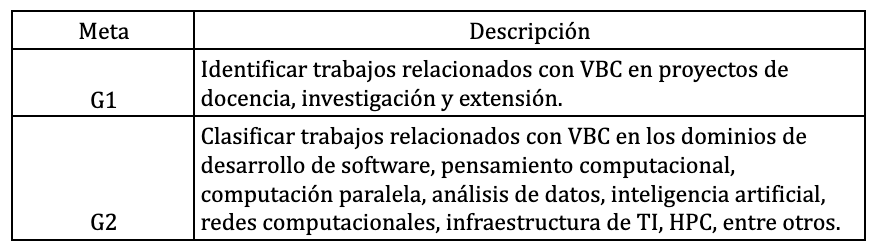
\includegraphics[width=\textwidth] {tablas-images/cp2/definicionMetas.png}
    \caption{Definición de metas del SMS}\label{tab:tabla-metas}
\end{table}

\subsubsection*{1.1.2 Definición de preguntas de investigación}
\addcontentsline{toc}{subsubsection}{Definición de preguntas de investigación}\label{subsubsec:preguntasInvestigacion}

\begin{table}[H]
    \centering
    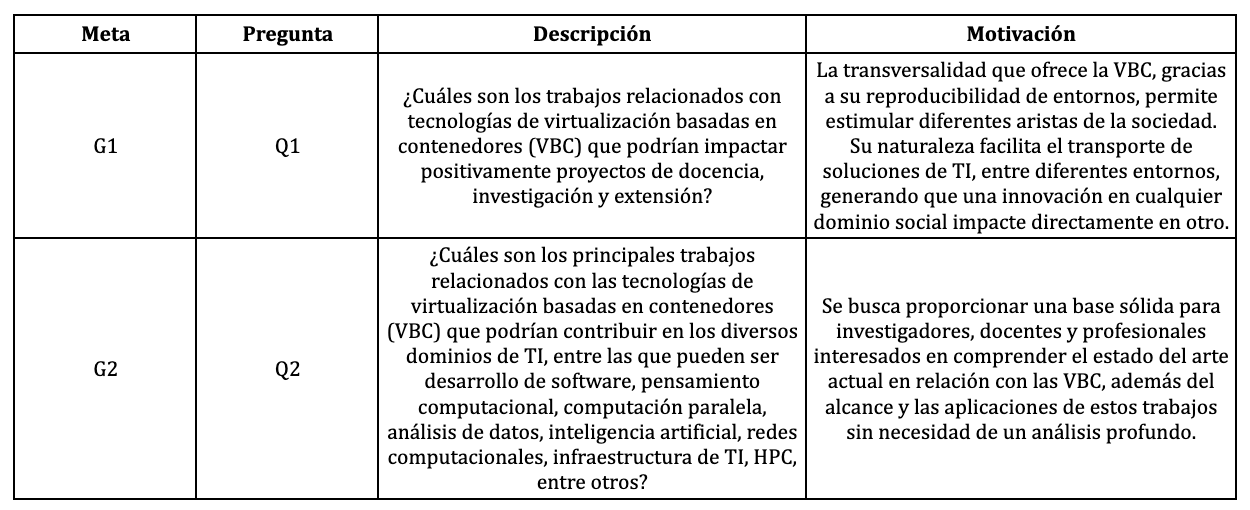
\includegraphics[width=\textwidth] {tablas-images/cp2/preguntasInvestigacion.png}
    \caption{Definición de preguntas de investigación del SMS}\label{tab:tabla-preguntas}
\end{table}

\subsubsection*{1.1.3 Definición de métricas}
\addcontentsline{toc}{subsubsection}{Definición de métricas}\label{subsubsec:metricasSMS}

\begin{figure}[H]
    \centering
    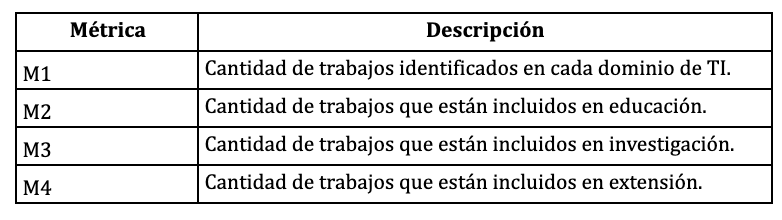
\includegraphics[width=\textwidth] {tablas-images/cp2/definicionMetricas.png}
    \caption{Definición de métricas del SMS}\label{fig:tabla-metricas}
\end{figure}

\section*{2. Búsqueda de estudios}
\addcontentsline{toc}{section}{Búsqueda de estudios}\label{sec:busquedaEstudios}

Esta etapa comprendió las siguientes secciones: 
\begin{enumerate}
  \item Estrategia de búsqueda, ya sea independiente o combinada;
  \item Identificación general de estudios;
  \item Selección; y finalmente,
  \item Selección de estudios para incluir en el SMS.\end{enumerate}

\subsection*{2.1 Estrategia de búsqueda}
\addcontentsline{toc}{subsection}{Estrategia de búsqueda}\label{subsec:estrategiaBusqueda}

Este trabajo combinó las estrategias de búsqueda en bases de datos y búsqueda en bola de nieve. 
Para la estrategia de búsqueda en bases de datos, se seleccionaron las siguientes bases de datos: ACM, IEEE Xplore, Springer, Taylor \& Francis y Science Direct.

\subsection*{2.2 Búsqueda en bases de datos}
\addcontentsline{toc}{subsection}{Búsqueda en bases de datos}\label{subsec:busquedaBasesDatos}
Se seleccionaron las siguientes bases de datos para este propósito: ACM, IEEE Xplore, Springer, Taylor \& Francis y Science Direct.

\subsubsection*{2.2.1 Identificación de estudios mediante búsqueda en bases de datos}
\addcontentsline{toc}{subsubsection}{Identificación de estudios mediante búsqueda en bases de datos}\label{subsubsec:identificacionEstudios}
En esta etapa del proceso fue necesario establecer las palabras clave que serían útiles en las cadenas de búsqueda para cada una de las bases de datos seleccionadas. 
Los términos consideran los elementos identificados en la etapa de planificación, para lo cual también se utilizó el modelo PICOC como guía metodológica.

\begin{table}[H]
    \centering
    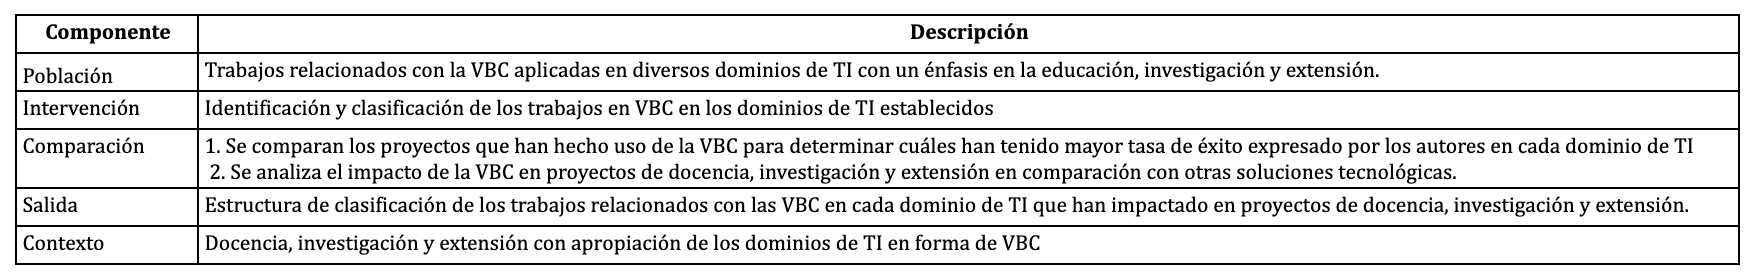
\includegraphics[width=\textwidth] {tablas-images/cp2/modelo-PICOC.png}
    \caption{Modelo PICOC}\label{tab:tabla-PICOC}
\end{table}
\begin{table}[H]
    \centering
    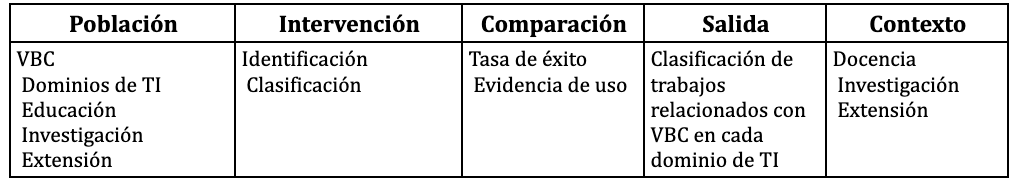
\includegraphics[width=\textwidth] {tablas-images/cp2/keywords-PICOC.png}
    \caption{Palabras clave identificadas usando el modelo PICOC}\label{tab:tabla-keywords-PICOC}
\end{table}
\begin{table}[H]
    \centering
    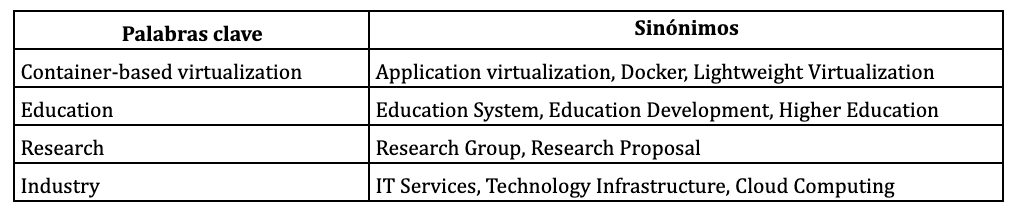
\includegraphics[width=\textwidth] {tablas-images/cp2/keywords.png}
    \caption{Palabras clave para la búsqueda en base de datos}\label{tab:tabla-keywords}
\end{table}
\begin{table}[H]
    \centering
    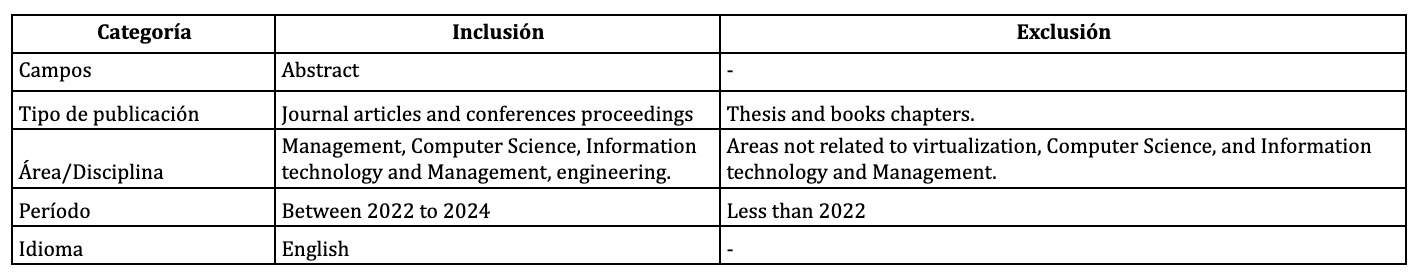
\includegraphics[width=\textwidth] {tablas-images/cp2/criterios.png}
    \caption{Criterios de Inclusión/Exclusión}\label{tab:tabla-criterios}
\end{table}

\subsubsection*{2.2.1.1 Búsqueda en bases de datos}
\addcontentsline{toc}{paragraph}{2.2.1.1 Búsqueda en bases de datos}\label{par:busquedaBasesDatos}

\begin{tcolorbox}[
  colback=gray!5, 
  colframe=black!60, 
  title=Cadena de búsqueda en ACM para educación, 
  fonttitle=\bfseries, 
  sharp corners=south
]
\scriptsize % o \footnotesize, \tiny según lo pequeño que lo quieras
\begin{verbatim}
(Title:("Container-based virtualization" OR "Application virtualization" OR "Docker" OR 
"Lightweight Virtualization") AND Title:("Education" OR "Education System" 
OR "Education Development" OR "Higher Education") ) 

OR

(Abstract:("Container-based virtualization" OR "Application virtualization" OR "Docker"
 OR "Lightweight Virtualization") AND Abstract:("Education" OR "Education System" 
 OR "Education Development" OR "Higher Education") )

OR

(Keyword:("Container-based virtualization" OR "Application virtualization" OR "Docker" OR 
"Lightweight Virtualization")
AND Keyword:("Education" OR "Education System" OR "Education Development" 
OR "Higher Education"))
\end{verbatim}
\end{tcolorbox}

\begin{tcolorbox}[
  colback=gray!5, 
  colframe=black!60, 
  title=Cadena de búsqueda en ACM para investigación, 
  fonttitle=\bfseries, 
  sharp corners=south
]
\scriptsize % puedes usar \tiny para hacerlo aún más pequeño
\begin{verbatim}
(Title:("Container-based virtualization" OR "Application virtualization" OR "Docker" OR 
"Lightweight Virtualization") AND Title:("Research" OR "Research Group" OR 
"Research Proposal"))

OR

(Abstract:("Container-based virtualization" OR "Application virtualization" OR "Docker" OR 
"Lightweight Virtualization") AND Abstract:("Research" OR "Research Group" OR 
"Research Proposal"))

OR

(Keyword:("Container-based virtualization" OR "Application virtualization" OR "Docker" OR 
"Lightweight Virtualization") AND Keyword:("Research" OR "Research Group" OR 
"Research Proposal"))
\end{verbatim}
\end{tcolorbox}

\begin{tcolorbox}[
  colback=gray!5, 
  colframe=black!60, 
  title=Cadena de búsqueda en ACM para industria, 
  fonttitle=\bfseries, 
  sharp corners=south
]
\scriptsize % puedes usar \tiny para hacerlo aún más pequeño
\begin{verbatim}
(Title:("Container-based virtualization" OR "Application virtualization" OR "Docker" OR 
"Lightweight Virtualization") AND Title:("Industry" OR “IT Services” OR 
“Technology Infrastructure” OR “Cloud Computing”) ) 

OR

(Abstract:("Container-based virtualization" OR "Application virtualization" OR "Docker" 
OR "Lightweight Virtualization") AND Abstract:("Industry" OR “IT Services” OR 
“Technology Infrastructure” OR “Cloud Computing”) )

OR

(Keyword:("Container-based virtualization" OR "Application virtualization" OR "Docker" 
OR "Lightweight Virtualization")
AND Keyword:("Industry" OR “IT Services” OR “Technology Infrastructure” 
OR “Cloud Computing”))

\end{verbatim}
\end{tcolorbox}

\begin{tcolorbox}[
  colback=gray!5, 
  colframe=black!60, 
  title=Cadena de búsqueda en IEE para educación, 
  fonttitle=\bfseries, 
  sharp corners=south
]
\scriptsize % puedes usar \tiny para hacerlo aún más pequeño
\begin{verbatim}
(("Abstract":"Container-based virtualization" OR "Abstract":"Application virtualization" 
OR "Abstract":"Docker" OR "Abstract":"Lightweight Virtualization") AND ("Abstract":"Education" 
OR "Abstract":"Education System" OR "Abstract":"Education Development”  OR 
"Abstract":"Higher Education”)) 

OR (("Publication Title":"Container-based virtualization" OR "Publication 
Title":"Application virtualization" 
OR "Publication Title":"Docker" OR "Publication Title":"Lightweight Virtualization") 
AND ("Publication Title":"Education" 
OR "Publication Title":"Education System" OR "Publication Title":"Education Development”  
OR "Publication Title":"Higher Education” ))

OR (("Author Keywords":"Container-based virtualization" OR 
"Author Keywords":"Application virtualization" OR 
"Author Keywords":"Docker" OR "Author Keywords":"Lightweight Virtualization") AND 
("Author Keywords":"Education" 
OR "Author Keywords":"Education System" OR "Author Keywords":"Education Development”  
OR "Author Keywords":"Higher Education”))
\end{verbatim}
\end{tcolorbox}


\begin{tcolorbox}[
  colback=gray!5, 
  colframe=black!60, 
  title=Cadena de búsqueda en IEE para investigación, 
  fonttitle=\bfseries, 
  sharp corners=south
]
\scriptsize % puedes usar \tiny para hacerlo aún más pequeño
\begin{verbatim}
(("Abstract":"Container-based virtualization" OR "Abstract":"Application virtualization" 
OR "Abstract":"Docker" OR "Abstract":"Lightweight Virtualization") AND 
("Abstract":"Research Group" OR "Abstract":"Research Proposal")) 

OR (("Publication Title":"Container-based virtualization" OR 
"Publication Title":"Application virtualization" OR "Publication Title":"Docker" OR 
"Publication Title":"Lightweight Virtualization") AND 
("Publication Title":"Research Group" OR "Publication Title":"Research Proposal" ))

OR (("Author Keywords":"Container-based virtualization" OR 
"Author Keywords":"Application virtualization" OR "Author Keywords":"Docker" OR 
"Author Keywords":"Lightweight Virtualization") AND 
("Author Keywords":"Research Group" OR "Author Keywords":"Research Proposal"))
\end{verbatim}
\end{tcolorbox}

\begin{tcolorbox}[
  colback=gray!5, 
  colframe=black!60, 
  title=Cadena de búsqueda en IEE para industria, 
  fonttitle=\bfseries, 
  sharp corners=south
]
\scriptsize % puedes usar \tiny para hacerlo aún más pequeño
\begin{verbatim}
(("Abstract":"Container-based virtualization" OR "Abstract":"Application virtualization" 
OR "Abstract":"Docker" OR "Abstract":"Lightweight Virtualization") AND 
("Abstract":"Industry" OR "Abstract":"IT Services" OR 
"Abstract":"Technology Infrastructure" OR "Abstract":"Cloud Computing")) 

OR (("Publication Title":"Container-based virtualization" OR 
"Publication Title":"Application virtualization" 
OR "Publication Title":"Docker" OR "Publication Title":"Lightweight Virtualization") AND 
("Publication Title":"Industry" OR "Publication Title":"IT Services" OR 
"Publication Title":"Technology Infrastructure" OR "Publication Title":"Cloud Computing"))

OR (("Author Keywords":"Container-based virtualization" OR 
"Author Keywords":"Application virtualization" OR "Author Keywords":"Docker" OR 
"Author Keywords":"Lightweight Virtualization") AND ("Author Keywords":"Industry" OR 
"Author Keywords":"IT Services" OR "Author Keywords":"Technology Infrastructure" OR 
"Author Keywords":"Cloud Computing"))
\end{verbatim}
\end{tcolorbox}

\begin{tcolorbox}[
  colback=gray!5, 
  colframe=black!60, 
  title=Cadena de búsqueda en Springer para educación, 
  fonttitle=\bfseries, 
  sharp corners=south
]
\scriptsize % puedes usar \tiny para hacerlo aún más pequeño
\begin{verbatim}
(title:("Container-based virtualization" OR "Application virtualization" OR 
"Docker" OR "Lightweight Virtualization") AND title:("Education" OR 
"Education System" OR "Education Development" OR "Higher Education"))

OR

(abstract:("Container-based virtualization" OR "Application virtualization" OR 
"Docker" OR "Lightweight Virtualization") AND abstract:("Education" OR 
"Education System" OR "Education Development" OR "Higher Education"))

OR 

(keyword:("Container-based virtualization" OR "Application virtualization" OR 
"Docker" OR "Lightweight Virtualization") AND keyword:("Education" OR 
"Education System" OR "Education Development" OR "Higher Education"))

\end{verbatim}
\end{tcolorbox}

\begin{tcolorbox}[
  colback=gray!5, 
  colframe=black!60, 
  title=Cadena de búsqueda en Springer para investigación, 
  fonttitle=\bfseries, 
  sharp corners=south
]
\scriptsize % puedes usar \tiny para hacerlo aún más pequeño
\begin{verbatim}
(title:("Container-based virtualization" OR "Application virtualization" OR 
"Docker" OR "Lightweight Virtualization") AND title:("research" OR 
"Research Group" OR "Research Proposal"))

OR

(abstract:("Container-based virtualization" OR "Application virtualization" 
OR "Docker" OR "Lightweight Virtualization") AND abstract:("research" 
OR "Research Group" OR "Research Proposal"))

OR 

(keyword:("Container-based virtualization" OR "Application virtualization"
 OR "Docker" OR "Lightweight Virtualization") AND keyword:("research" OR 
 "Research Group" OR "Research Proposal"))

\end{verbatim}
\end{tcolorbox}

\begin{tcolorbox}[
  colback=gray!5, 
  colframe=black!60, 
  title=Cadena de búsqueda en Springer para industria, 
  fonttitle=\bfseries, 
  sharp corners=south
]
\scriptsize % puedes usar \tiny para hacerlo aún más pequeño
\begin{verbatim}
(title:("Container-based virtualization" OR "Application virtualization"
 OR "Docker" OR "Lightweight Virtualization") AND title:("Industry" OR 
 “IT Services” OR “Technology Infrastructure” OR “Cloud Computing”))

OR

(abstract:("Container-based virtualization" OR "Application virtualization" 
OR "Docker" OR "Lightweight Virtualization") AND abstract:("Industry" OR 
“IT Services” OR “Technology Infrastructure” OR “Cloud Computing”))

OR 

(keyword:("Container-based virtualization" OR "Application virtualization"
 OR "Docker" OR "Lightweight Virtualization") AND keyword:("Industry" 
 OR “IT Services” OR “Technology Infrastructure” OR “Cloud Computing”))

\end{verbatim}
\end{tcolorbox}

\begin{tcolorbox}[
  colback=gray!5, 
  colframe=black!60, 
  title=Cadena de búsqueda en Science Direct para educación, 
  fonttitle=\bfseries, 
  sharp corners=south
]
\scriptsize % puedes usar \tiny para hacerlo aún más pequeño
\begin{verbatim}
("Container-based virtualization" OR "Application virtualization" 
OR "Docker" OR "Lightweight Virtualization")  AND ("Education" OR 
"Education System" OR "Education Development" OR "Higher Education")
\end{verbatim}
\end{tcolorbox}


\begin{tcolorbox}[
  colback=gray!5, 
  colframe=black!60, 
  title=Cadena de búsqueda en Science Direct para investigación, 
  fonttitle=\bfseries, 
  sharp corners=south
]
\scriptsize % puedes usar \tiny para hacerlo aún más pequeño
\begin{verbatim}
("Container-based virtualization" OR "Application virtualization" OR 
"Docker" OR "Lightweight Virtualization")  AND ("Research" OR 
"Research Group" OR "Research Proposal")
\end{verbatim}
\end{tcolorbox}

\begin{tcolorbox}[
  colback=gray!5, 
  colframe=black!60, 
  title=Cadena de búsqueda en Science Direct para industria, 
  fonttitle=\bfseries, 
  sharp corners=south
]
\scriptsize % puedes usar \tiny para hacerlo aún más pequeño
\begin{verbatim}
("Container-based virtualization" OR "Application virtualization" OR "Docker" OR 
"Lightweight Virtualization")  AND 
(“Industry” OR "IT Services" OR "Technology Infrastructure" OR "Cloud Computing")
\end{verbatim}
\end{tcolorbox}

\begin{tcolorbox}[
  colback=gray!5, 
  colframe=black!60, 
  title=Cadena de búsqueda en Taylor \& Francis para educación, 
  fonttitle=\bfseries, 
  sharp corners=south
]
\scriptsize % puedes usar \tiny para hacerlo aún más pequeño
\begin{verbatim}
("Application virtualization" OR "Docker" OR "Lightweight Virtualization" OR "Docker Container")   
AND   
("Education System" OR "Education Sector" OR "Education Development" OR "Higher Education")
\end{verbatim}
\end{tcolorbox}

\begin{tcolorbox}[
  colback=gray!5, 
  colframe=black!60, 
  title=Cadena de búsqueda en Taylor \& Francis para investigación, 
  fonttitle=\bfseries, 
  sharp corners=south
]
\scriptsize % puedes usar \tiny para hacerlo aún más pequeño
\begin{verbatim}
("Application virtualization" OR "Docker" OR "Lightweight Virtualization" OR "Docker Container")
AND   
("Specific Research Areas" OR "Research Group" OR "Research Proposal" OR "Research and Development")
\end{verbatim}
\end{tcolorbox}

\begin{tcolorbox}[
  colback=gray!5, 
  colframe=black!60, 
  title=Cadena de búsqueda en Taylor \& Francis para industria, 
  fonttitle=\bfseries, 
  sharp corners=south
]
\scriptsize % puedes usar \tiny para hacerlo aún más pequeño
\begin{verbatim}
("Application virtualization" OR "Docker" OR "Lightweight Virtualization" OR "Docker Container")  
AND 
(“Industry” OR "IT Services" OR "Technology Infrastructure" OR "Cloud Computing")
\end{verbatim}
\end{tcolorbox}

\subsubsection*{2.2.2 Resumen de la búsqueda en bases de datos sin criterios de inclusión/exclusión}
\addcontentsline{toc}{subsubsection}{Resumen de la búsqueda en bases de datos sin criterios de inclusión/exclusión}\label{subsubsec:resumenBusqueda}
Este es el resultado antes de aplicar criterios de exclusión

\begin{table}[H]
    \centering
    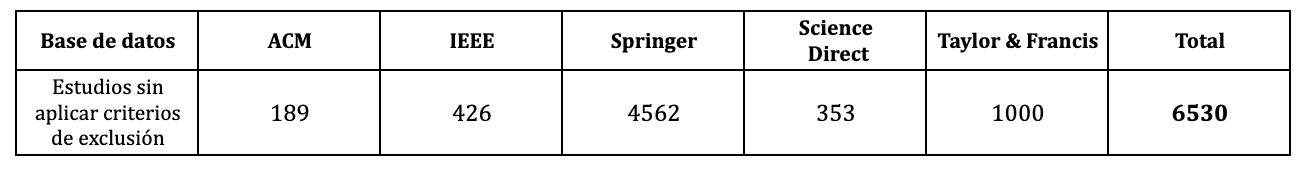
\includegraphics[width=\textwidth] {tablas-images/cp2/resumen-sin-criterios.png}
    \caption{Resumen de la búsqueda en bases de datos sin criterios de inclusión/exclusión}\label{tab:tabla-resumen-sin-criterios}
\end{table}
\begin{figure}[H]
    \centering
    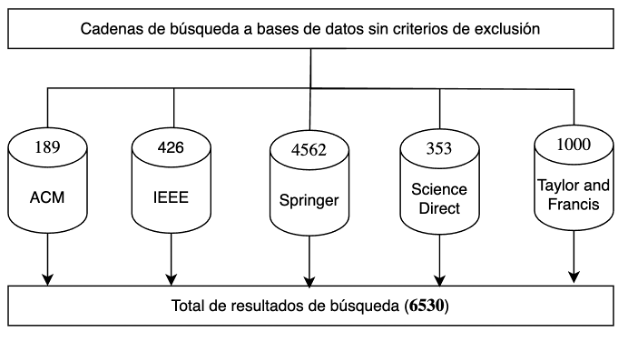
\includegraphics[scale=0.9]{tablas-images/cp2/bases-sin-criterio.png}
    \caption{Diagrama de búsqueda en bases de datos}\label{fig:tabla-resumen-busqueda}
\end{figure}

\subsubsection*{2.2.3	Aplicación de criterios de exclusión de las bases de datos}
Esta búsqueda se realizó considerando los criterios de exclusión e inclusión definidos previamente.

Las cadena de búsqueda son exactamente iguales que antes, este punto se diferencia por la aplicación de 
filtros. Para ver las capturas de pantalla veáse el apéndice B sección 2.

\subsection*{2.3 Resumen de la búsqueda en bases de datos con criterios de inclusión/exclusión}
\addcontentsline{toc}{subsection}{Resumen de la búsqueda en bases de datos con
    criterios de inclusión/exclusión}\label{subsec:resumenBusquedaCriterios}

\begin{table}[H]
\centering
\scriptsize
\setlength{\tabcolsep}{4pt}
\renewcommand{\arraystretch}{1.1}
\begin{tabular}{|l|c|c|c|c|c|c|}
\hline
\textbf{Bases de datos} & \textbf{ACM} & \textbf{IEEE} & \textbf{Springer} & \textbf{Science Direct} & \textbf{Taylor \& Francis} & \textbf{Total} \\
\hline
Con criterios aplicados & 48 & 134 & 592 & 46 & 156 & 976 \\
\hline
\end{tabular}
\caption{Resumen de la búsqueda en bases de datos con criterios de inclusión/exclusión}\label{tab:resumen-busqueda}
\end{table}
\begin{figure}[H]
    \centering
    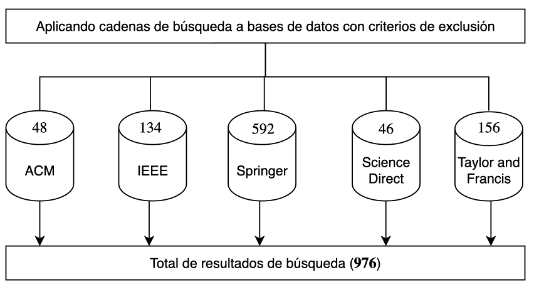
\includegraphics[width=\textwidth] {tablas-images/cp2/bases-con-criterio.png}
    \caption{Resumen de la búsqueda en bases de datos con criterios de inclusión/exclusión}\label{fig:tabla-resumen-busqueda-con-criterio}
\end{figure}

\section*{3 Eliminación de duplicados}
\addcontentsline{toc}{section}{Eliminación de duplicados}\label{sec:eliminacionDuplicados}
La eliminación de duplicados se realizó haciendo uso de la herramienta de gestión de referencias Mendeley. Luego de obtener los artículos se agregaron a Mendeley y esta herramienta se encargó de eliminar duplicados. En este punto se eliminaron 274 artículos duplicados.

\section*{4 Priorización de estudios}
\addcontentsline{toc}{section}{Priorización de estudios}\label{sec:priorizacionEstudios}

Luego de la selección inicial de los artículos, se procedió a revisar el \textit{title}, \textit{abstract} y \textit{keywords} de cada uno. Como resultado de esta revisión, se generaron métricas de calidad para cada artículo, con el fin de priorizar aquellos más relevantes para la investigación. Las métricas utilizadas fueron las siguientes:

\begin{itemize}
    \item \textbf{SCI} (Science Citation Index)
    \item \textbf{CVI} (Core Value Index)
    \item \textbf{IRRQ} (Index Relation Research Question)
\end{itemize}

Este proceso inició con un total de 771 artículos, los cuales fueron evaluados según su alineamiento con los objetivos de la investigación. La evaluación temática permitió identificar un total de 110 artículos con una relación directa con el enfoque planteado.

\section*{5 Estrategia de búsqueda usando bola de nieve}
\addcontentsline{toc}{section}{Estrategia de búsqueda usando bola de nieve}\label{sec:bolaDeNieve}

En esta etapa, se seleccionó el primer cuartil según el índice \textbf{IRRQ}, lo que resultó en un total de 24 artículos. Adicionalmente, se incluyeron dos artículos por criterio de inclusión directa, estableciendo así una línea base de \textbf{26 artículos}. 

Sobre esta base, se aplicó la estrategia de \textit{bola de nieve} en ambas direcciones: hacia adelante y hacia atrás. Como resultado, se obtuvieron \textbf{87 artículos} mediante la técnica hacia atrás y \textbf{495 artículos} mediante la técnica hacia adelante. 

Esto definió un nuevo conjunto de artículos para un proceso de selección adicional (\textit{screening}). En esta fase, se eliminaron \textbf{14 duplicados} y \textbf{452 artículos} fueron descartados por no estar alineados con la investigación. 

Finalmente, se obtuvo un total de \textbf{116 artículos} mediante esta estrategia de búsqueda ampliada.

\section*{6 Diagrama de búsqueda}
\addcontentsline{toc}{section}{Diagrama de búsqueda}\label{sec:diagramaBusqueda}

\subsection*{6.1 Usando cadenas de búsqueda}
\addcontentsline{toc}{subsection}{Usando cadenas de búsqueda}\label{subsec:cadenaBusqueda}
\begin{table}[H]
    \centering
    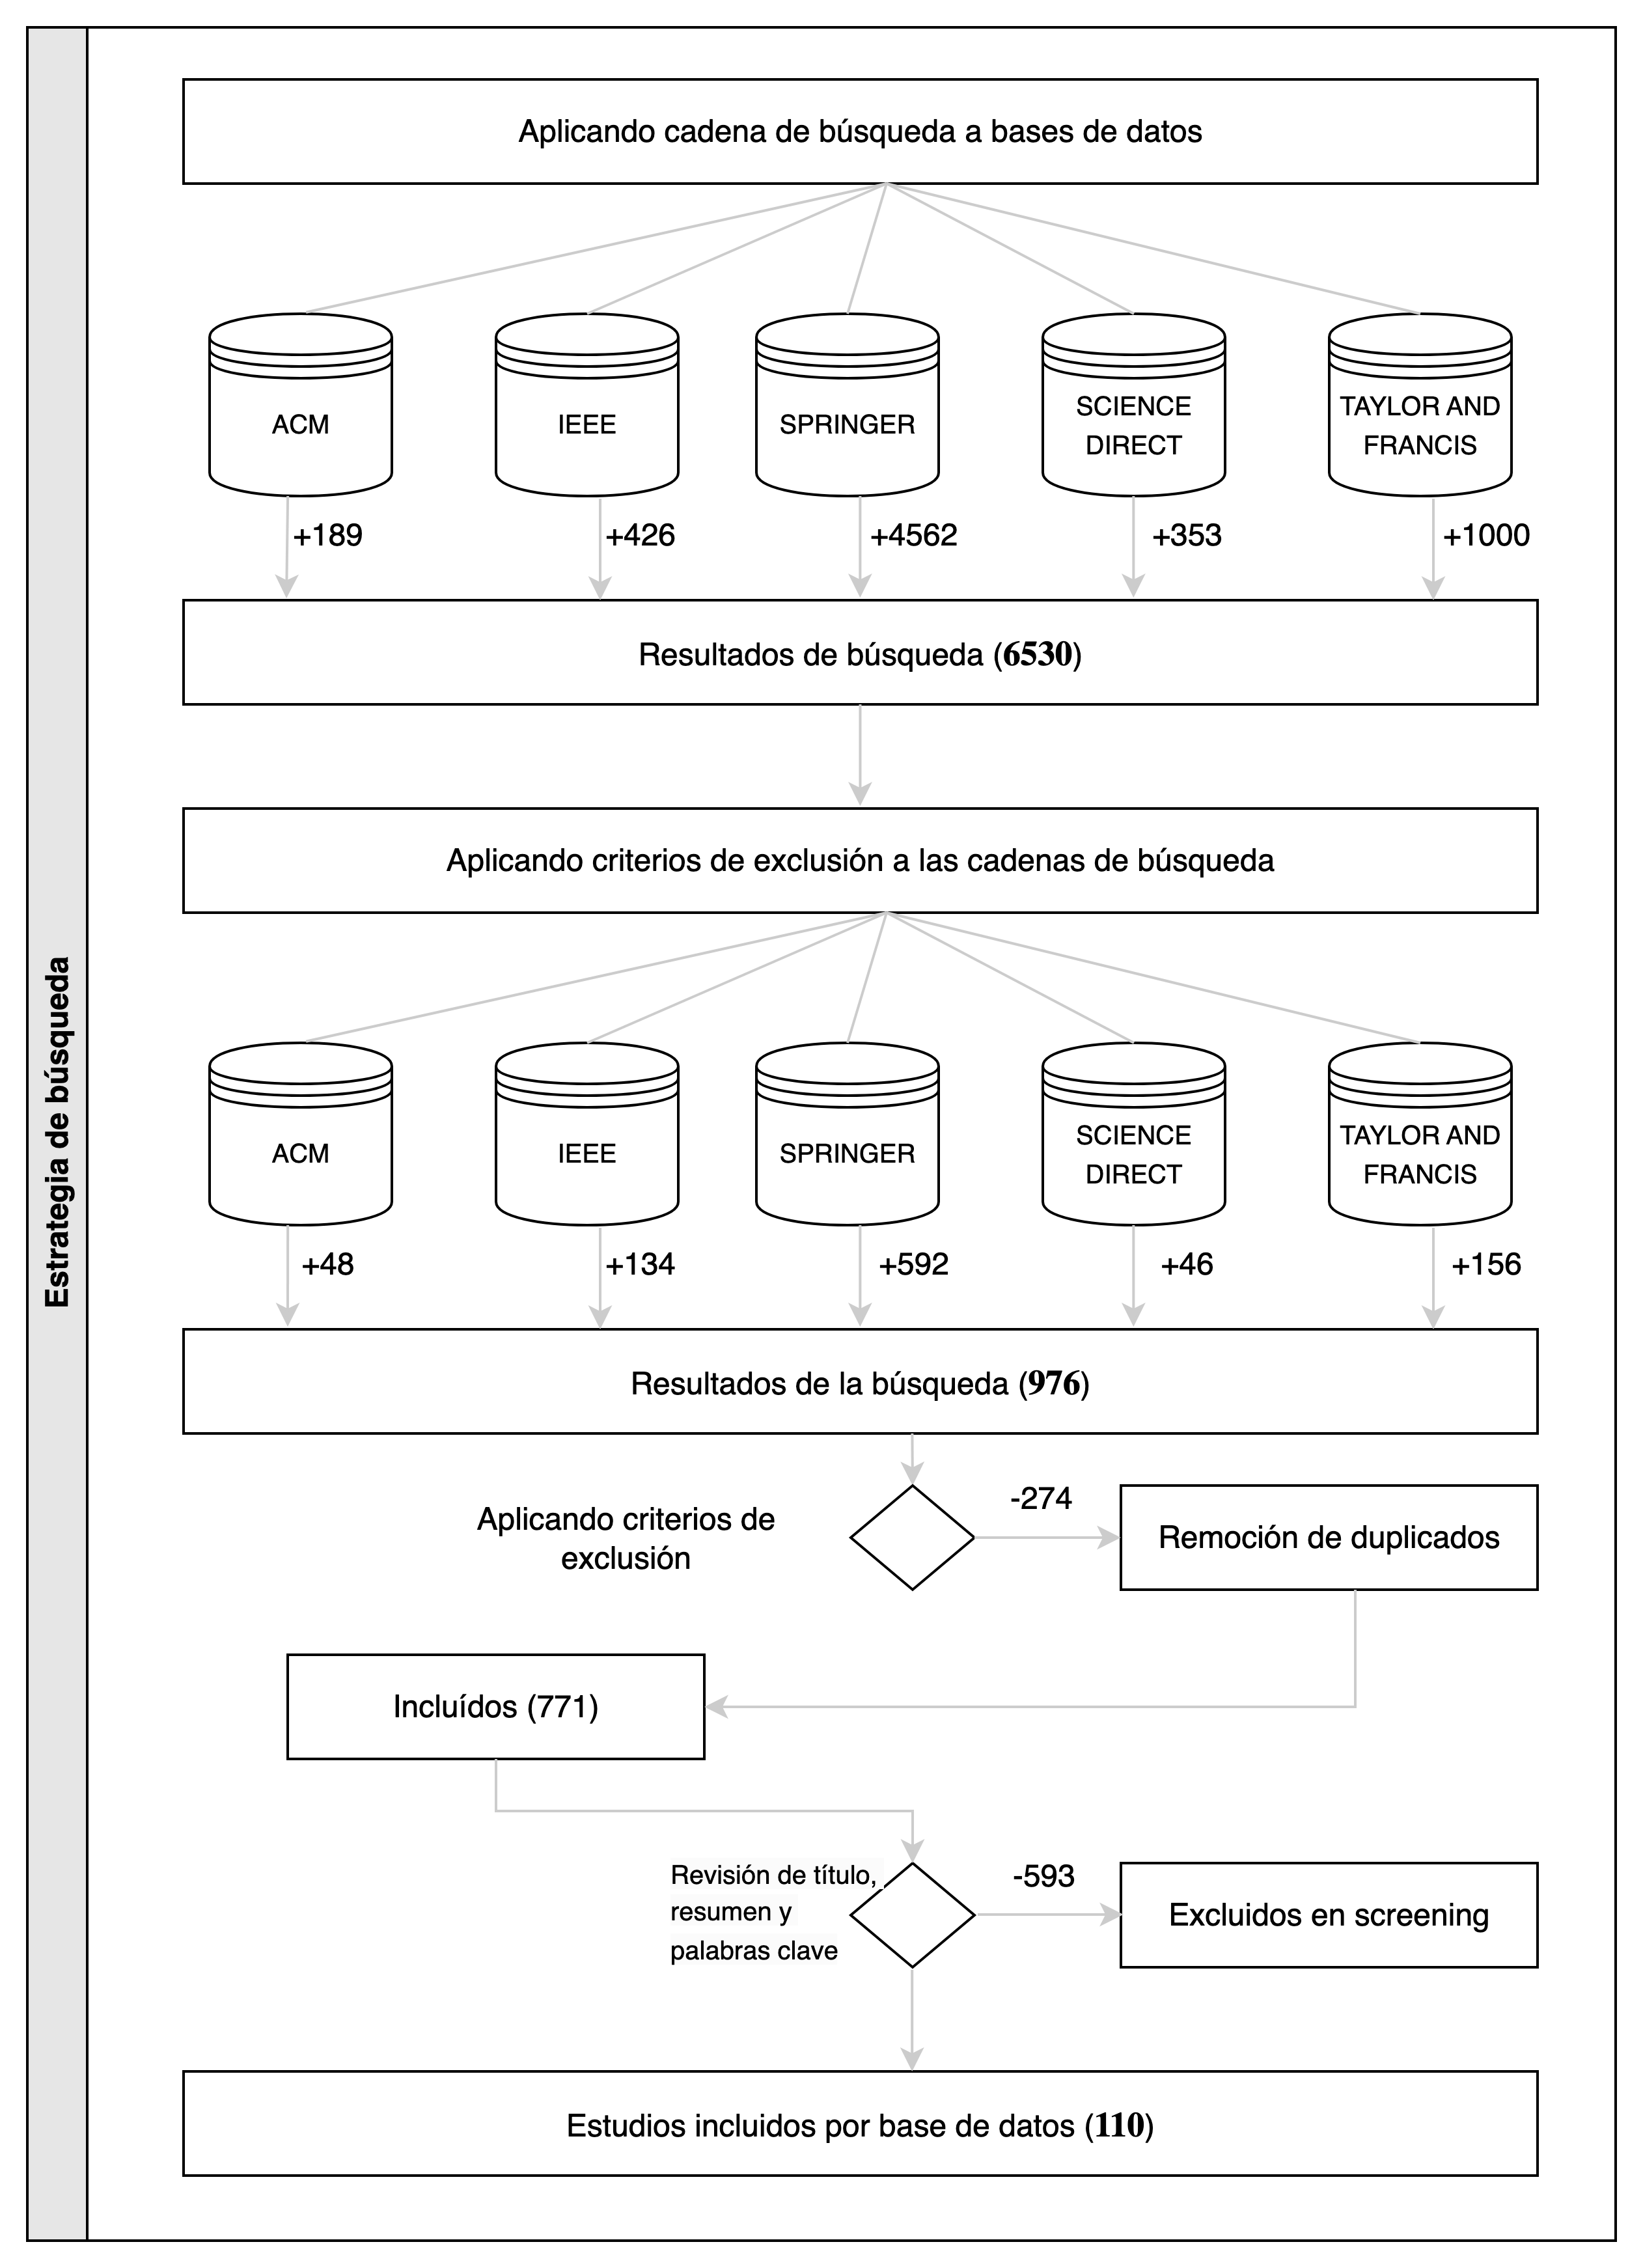
\includegraphics[scale=0.13]{tablas-images/cp2/diagrama-cadena-busqueda.png}
    \caption{Diagrama de la cadena de búsqueda}\label{tab:tabla-diagrama-cadena-busqueda}
\end{table}

\subsection*{6.2 Usando bola de nieve}
\addcontentsline{toc}{subsection}{Usando bola de nieve}\label{subsec:bolaNieveBusqueda}
\begin{table}[H]
    \centering
    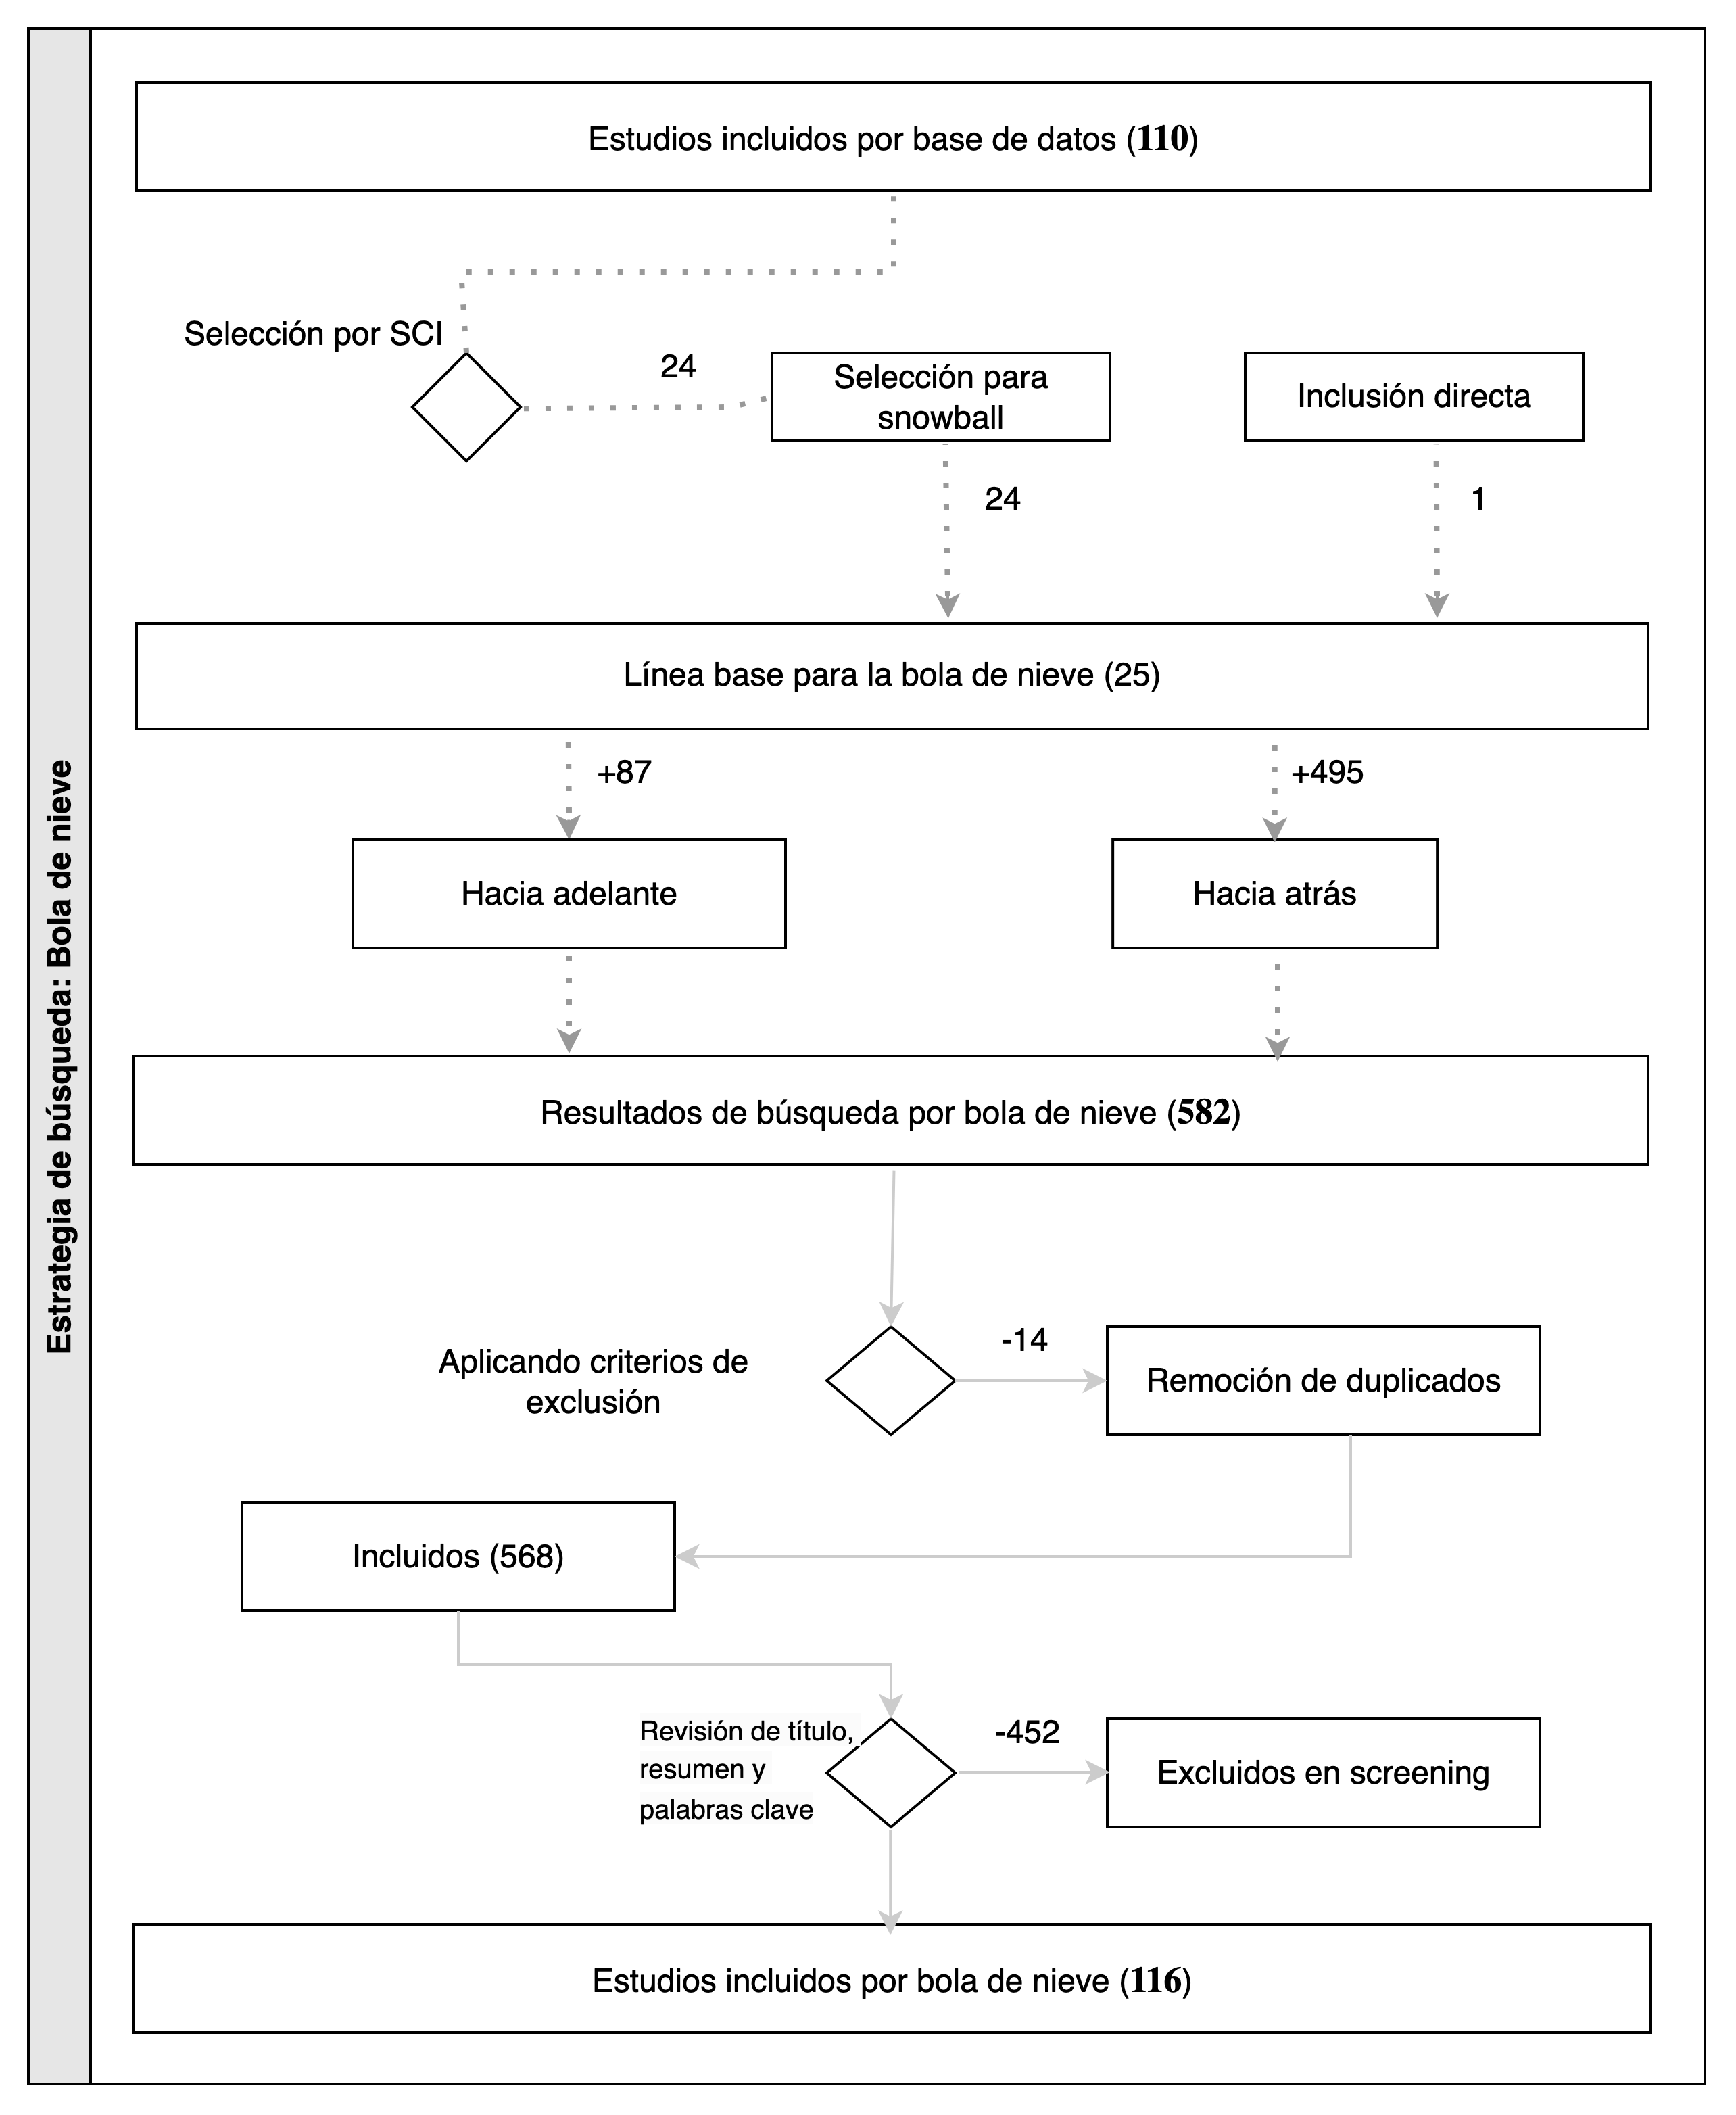
\includegraphics[scale=0.14]{tablas-images/cp2/diagrama-bola-nieve-busqueda.png}
    \caption{Diagrama de la búsqueda en bola de nieve}\label{tab:tabla-diagrama-bola-nieve-busqueda}
\end{table}

\section*{7 Identificación de estudios}
\addcontentsline{toc}{section}{Identificación de estudios}\label{sec:identificacionEstudios}

\subsection*{7.1 Artículos por año y métricas}
\addcontentsline{toc}{subsection}{Artículos por año y métricas}\label{subsec:articulosPorAnoYMetrica}
\begin{figure}[H]
    \centering
    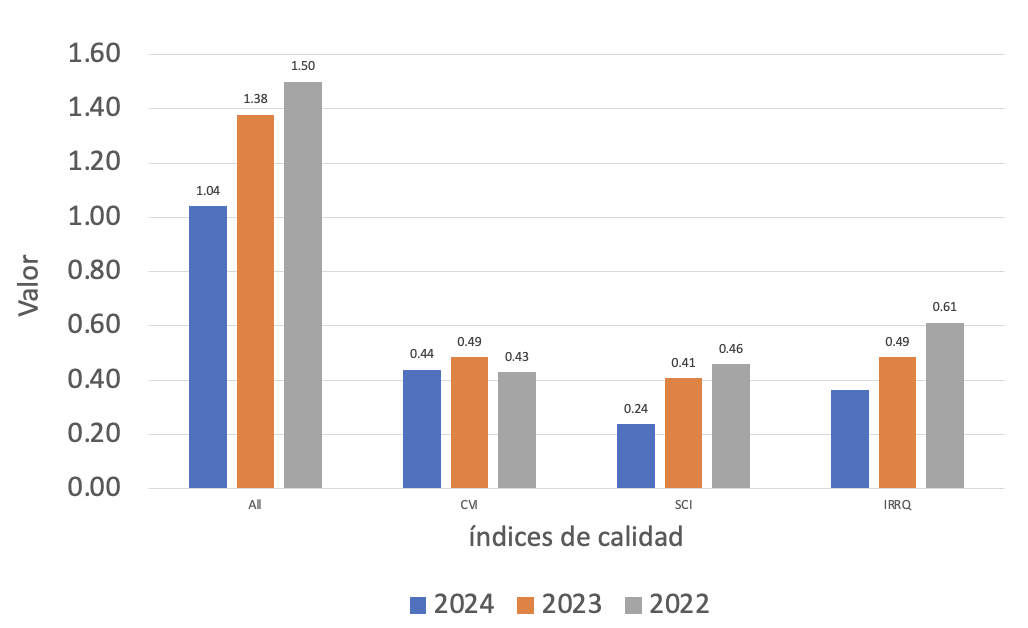
\includegraphics[width=\textwidth]{tablas-images/cp2/diagrama-articulos-ano-metrica.png}
    \caption{Artículos por métricas y año}\label{fig:diagrama-articulos-ano-metrica}
\end{figure}

\begin{figure}[H]
    \centering
    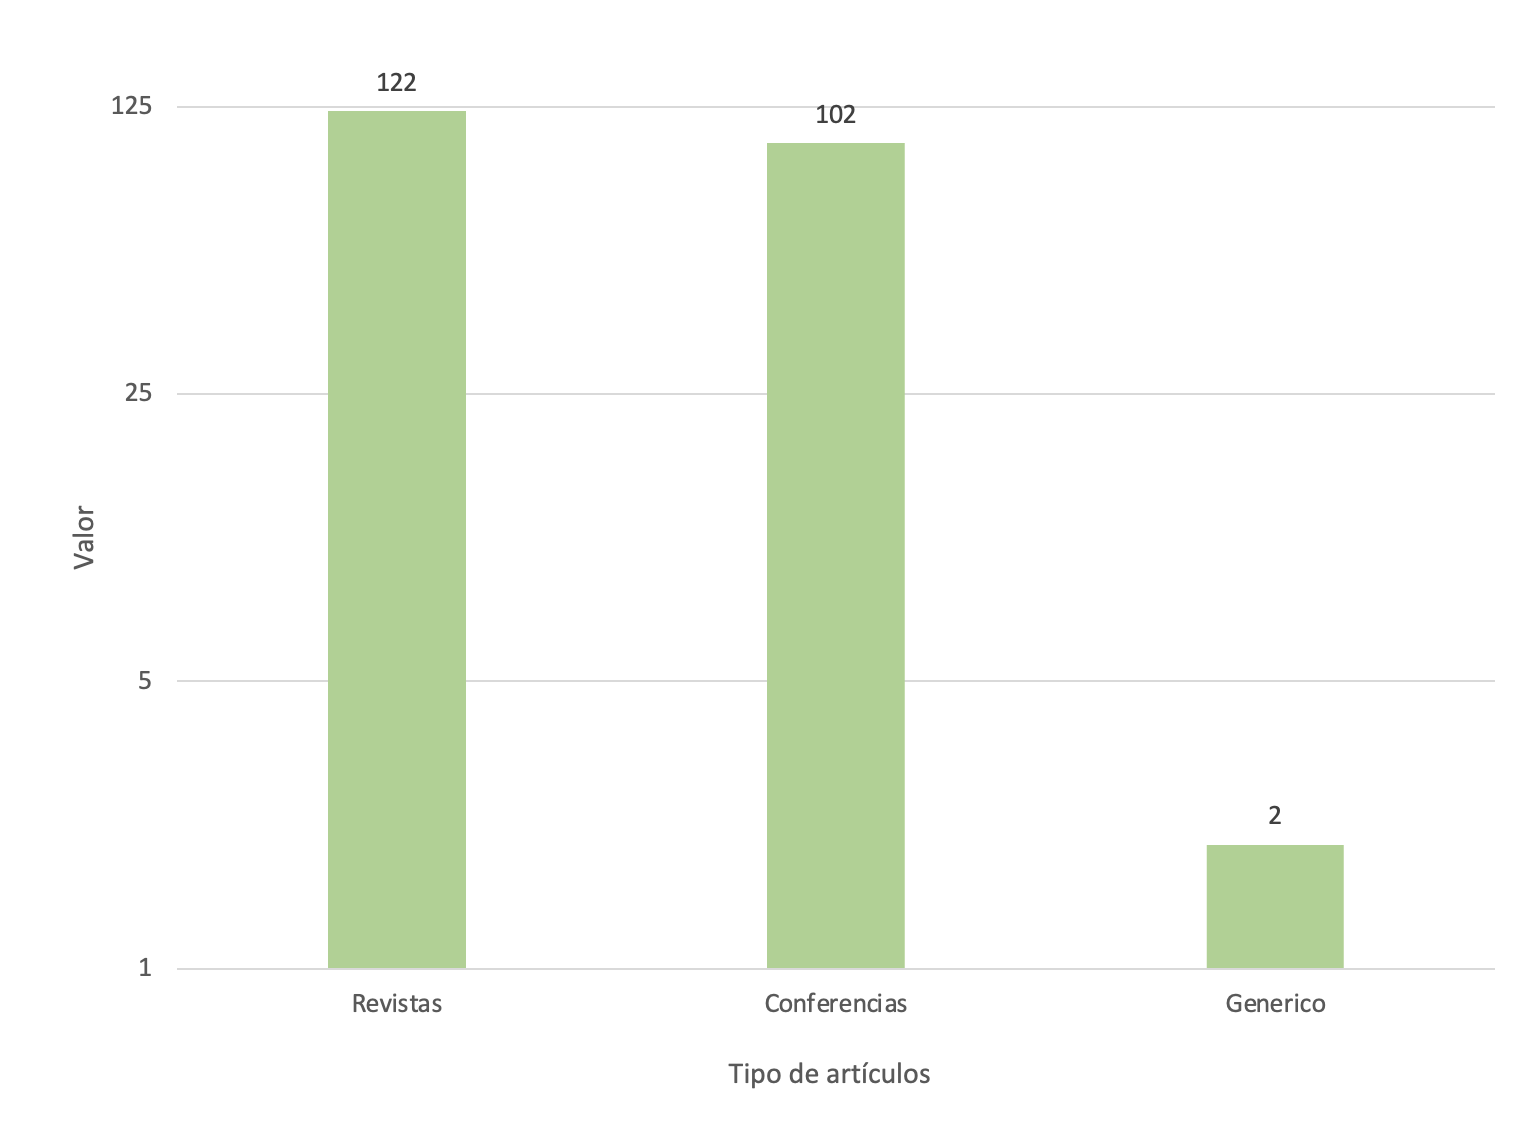
\includegraphics[width=\textwidth]{tablas-images/cp2/tipos-articulos.png}
    \caption{Artículos por tipo}\label{fig:tipos-articulos}
\end{figure}

\begin{figure}[H]
    \centering
    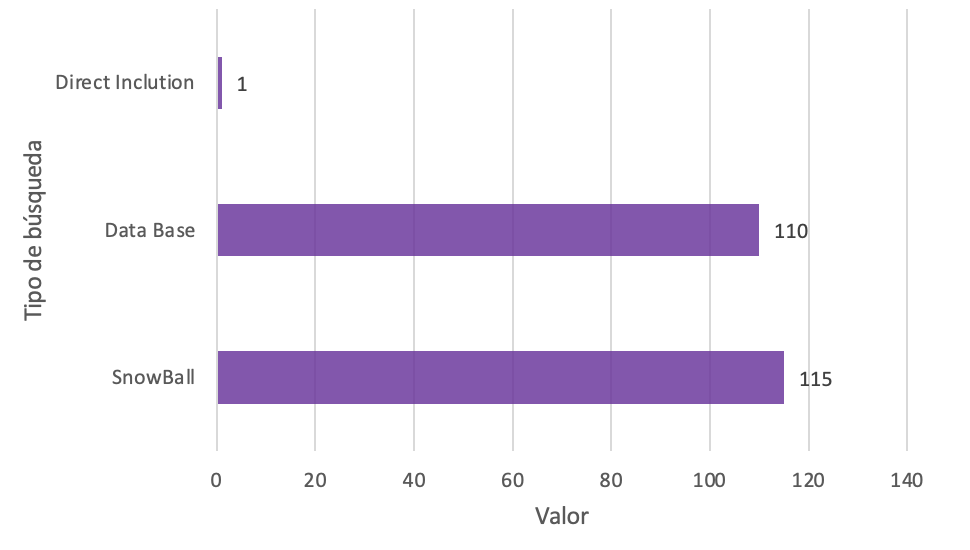
\includegraphics[width=\textwidth]{tablas-images/cp2/estrategia-busqueda-articulos.png}
    \caption{Estrategia de búsqueda de artículos}\label{fig:estrategia-busqueda-articulos}
\end{figure}

\begin{figure}[H]
    \centering
    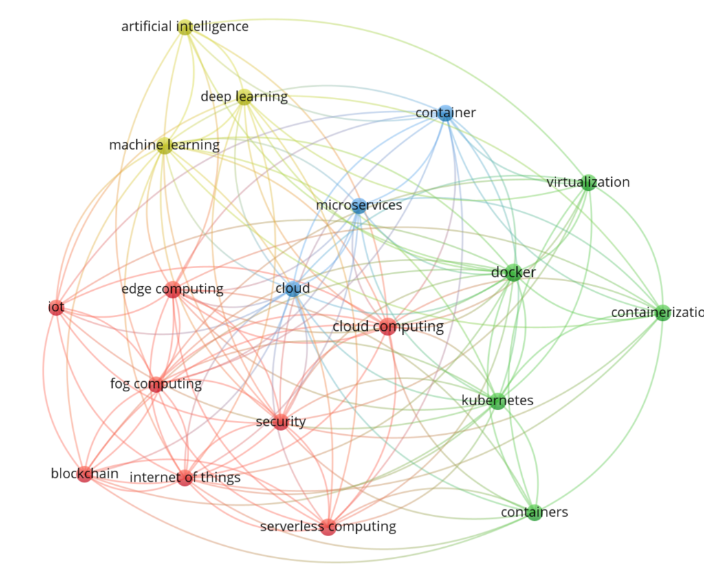
\includegraphics[width=\textwidth]{tablas-images/cp2/diagrama-red-busqueda.png}
    \caption{Diagrama de red de los artículos}\label{fig:diagrama-red-articulos}
\end{figure}

\section*{8 Información de la herramienta}
\addcontentsline{toc}{subsection}{Información de la herramienta}\label{subsec:informacionHerramienta}

\noindent
La herramienta utilizada para este proceso de revisión de la literatura fue \textbf{SMS-BUILDER}, la cual se encuentra disponible en \textit{Docker Hub}. El estudio realizado puede consultarse en el siguiente enlace:

\begin{center}
\href{https://sms-vbc.iti.grid.uniquindio.edu.co/}{\texttt{https://sms-vbc.iti.grid.uniquindio.edu.co/}}
\end{center}

\noindent
Adicionalmente, se implementaron procesos de respaldo como medida de seguridad. Estos \textit{backups} fueron almacenados en ubicaciones diferentes, siguiendo la estrategia de respaldo \textbf{3--2--1}.

\section{Nichos de mercado}

\subsection{Containerd}
\noindent
Containerd está dirigido a proveedores de servicios en la nube y plataformas de orquestación como Kubernetes, donde se requiere una solución de gestión de contenedores ligera y compatible con OCI \citep{Vano2023}. Su arquitectura modular lo convierte en una opción preferida para grandes infraestructuras \citep{Zhou2021}.

\subsection{CRI-O}
\noindent
CRI-O está diseñado específicamente para su integración con Kubernetes, sirviendo como un motor de contenedores ligero y compatible con OCI para esta plataforma \citep{CNCF2019}. Es una solución ideal para proveedores de servicios en la nube y organizaciones que utilizan Kubernetes como su plataforma de orquestación principal \citep{151962df5f7e4b9faba0629540c11439}.

\subsection{Docker}
\noindent
Docker se posiciona principalmente en el nicho de mercado de desarrolladores de software, empresas tecnológicas y proveedores de servicios en la nube que buscan una solución para la creación, implementación y gestión de aplicaciones en contenedores \citep{Hill2025}. Su capacidad de automatizar despliegues y la portabilidad entre entornos lo convierte en una opción ideal para DevOps y desarrollo ágil \citep{Mag2025}.

\subsection{Firecracker}
\noindent
Firecracker está orientado a proveedores de servicios en la nube y plataformas de cómputo en la nube que requieren micro VMs eficientes y seguras \citep{Jain}. Es una solución ideal para plataformas \textit{serverless} y entornos multi-tenant \citep{246288}.

\subsection{Google gVisor}
\noindent
Google gVisor está dirigido a proveedores de servicios en la nube y organizaciones que priorizan la seguridad en sus entornos de contenedores \citep{LopezFalcon2024}. Su arquitectura de \textit{sandbox} proporciona un aislamiento fuerte, lo que lo convierte en una opción atractiva para aplicaciones sensibles \citep{gvisor2025}.

\subsection{Hyper-V Containers}
\noindent
Hyper-V Containers están orientados a empresas que utilizan infraestructuras basadas en Windows, ofreciendo una solución de contenedorización segura y eficiente para aplicaciones basadas en Windows \citep{Smith2016}. Su integración con el ecosistema de Microsoft lo hace ideal para empresas con infraestructuras híbridas \citep{Clark2024}.

\subsection{Kata Containers}
\noindent
Kata Containers se centra en entornos donde se requiere un alto nivel de seguridad y aislamiento, como proveedores de servicios en la nube y empresas que manejan información confidencial \citep{Viktorsson2020}. Su capacidad para combinar la eficiencia de los contenedores con el aislamiento de máquinas virtuales es su principal ventaja \citep{10.1145/1272996.1273025}.

\subsection{Linux VServer}
\noindent
Linux VServer está orientado a administradores de sistemas y proveedores de servicios que requieren una solución de virtualización ligera basada en contenedores para la administración de servidores seguros y eficientes \citep{10.1145/1272996.1273025}. Es una opción adecuada para entornos de servidor dedicados y alojamientos compartidos \citep{LinuxVirt2017}.

\subsection{LXC (Linux Containers)}
\noindent
LXC es popular en entornos de virtualización ligera y servidores, donde se requiere un control granular sobre los entornos de contenedores \citep{Silva2024}. Su uso está orientado a proveedores de alojamiento web, desarrolladores de software y administradores de sistemas que necesitan un control preciso del entorno del sistema operativo \citep{Simon2023}.

\subsection{LXD}
\noindent
LXD se enfoca en nichos de mercado que requieren entornos de virtualización basados en contenedores que imiten máquinas virtuales, como proveedores de servicios en la nube, plataformas de pruebas y entornos de desarrollo \citep{Silva2024}. Su capacidad para ofrecer entornos de sistema completo lo hace ideal para desarrolladores y administradores de sistemas \citep{Kaiser2022}.

\subsection{OpenVZ}
\noindent
OpenVZ se centra en proveedores de alojamiento web y servicios VPS, donde se requiere una solución de virtualización ligera basada en contenedores que permita un control granular sobre los recursos del sistema y la administración de múltiples instancias \citep{OpenVZ2015}.

\subsection{Podman}
\noindent
Podman está orientado a entornos empresariales y desarrolladores que requieren una solución de contenerización sin \textit{daemon}, compatible con OCI y con enfoque en la seguridad \citep{Surendhar2024}. Su naturaleza sin \textit{daemon} y su capacidad para ejecutar contenedores de forma aislada permiten su adopción en entornos donde la seguridad y la conformidad son prioridades \citep{Trevor2022}.

\subsection{Rkt}
\noindent
Rkt fue diseñado para satisfacer las necesidades de proveedores de servicios en la nube y organizaciones que buscan una alternativa a Docker con un enfoque en la seguridad y compatibilidad OCI \citep{Lingayat2018}. Aunque su desarrollo ha sido discontinuado, sigue siendo relevante en entornos donde la compatibilidad y la seguridad son críticas \citep{Watada2019}.

\subsection{runC}
\noindent
runC está orientado a proveedores de servicios en la nube, plataformas de orquestación como Kubernetes y desarrolladores de software que buscan una solución de contenedorización ligera y compatible con OCI \citep{Perez2005}. Su adopción en proyectos de gran escala se debe a su eficiencia y cumplimiento de estándares de contenedores \citep{151962df5f7e4b9faba0629540c11439}.

\subsection{Sarus}
\noindent
Sarus está dirigido a entornos de HPC y computación científica, donde los usuarios necesitan ejecutar contenedores de forma segura en sistemas de alto rendimiento \citep{Sarus2021}. Su compatibilidad con estándares de contenedores y su enfoque en la seguridad lo hacen ideal para centros de investigación y universidades \citep{B2020}.

\subsection{Singularity}
\noindent
Singularity se centra en entornos de computación científica y HPC, donde se requiere portabilidad de aplicaciones sin necesidad de privilegios de root \citep{10.1145/3332186.3332192}. Es ampliamente adoptado en universidades, centros de investigación y laboratorios que ejecutan aplicaciones de alto rendimiento \citep{Kurtzer2017}.

\subsection{Udocker}
\noindent
Udocker se especializa en nichos de mercado académicos y de investigación, donde los usuarios necesitan ejecutar contenedores sin privilegios en sistemas que no permiten la instalación de software de nivel de sistema \citep{Campos2017}. Su facilidad para funcionar en entornos HPC (Computación de Alto Rendimiento) sin requerir permisos de root lo hace adecuado para instituciones de investigación \citep{Gomes2018}.

\subsection{Wasm (WebAssembly)}
\noindent
Wasm se centra en el nicho de desarrollo web y aplicaciones de alto rendimiento en el navegador \citep{Haas2017}. Su capacidad para ejecutar código en múltiples plataformas, incluidas aplicaciones de escritorio y móviles, lo convierte en una opción atractiva para empresas de desarrollo de software que buscan optimización multiplataforma \citep{Jangda2019}.
\clearpage
\section{Comparativa de licencias}
\noindent
La tabla~\ref{tab:licencias-vbc} presenta un panorama comparativo de las tecnologías de \VBC\ presentadas antes, detallando aspectos clave como el tipo de licencia, los términos de uso y los costos asociados. Este análisis permite identificar no solo las diferencias en cuanto a modelos de distribución y sostenibilidad económica, sino también las implicaciones legales y técnicas que pueden influir en la selección de una u otra herramienta en contextos de investigación o implementación empresarial. Asimismo, se evidencia la coexistencia de soluciones de código abierto, ampliamente utilizadas en entornos académicos y científicos, junto con alternativas propietarias que implican costos más elevados, lo cual resalta la necesidad de evaluar cuidadosamente la relación entre funcionalidad, libertad de uso y viabilidad financiera.
\begin{table}[H]
\centering
\scriptsize
\setlength{\tabcolsep}{3pt}
\renewcommand{\arraystretch}{1.1}
\begin{tabular}{|>{\centering\arraybackslash}m{0.18\textwidth}| 
                >{\centering\arraybackslash}m{0.25\textwidth}| 
                >{\centering\arraybackslash}m{0.20\textwidth}| 
                >{\centering\arraybackslash}m{0.25\textwidth}|}
\hline
\textbf{Tecnologías} & \textbf{Licencias} & \textbf{Términos de uso} & \textbf{Costo} \\
\hline
Docker & Apache 2.0 & \href{https://www.docker.com/legal/docker-terms-service/}{link} & \$11-\$24 \\
\hline
Podman & Apache 2.0 & \href{https://github.com/containers/podman/blob/main/LICENSE}{link} & Gratis \\
\hline
Udocker & Apache 2.0 & \href{https://github.com/indigo-dc/udocker/blob/master/LICENSE}{link} & Gratis \\
\hline
Wasm & Apache 2.0 & \href{https://github.com/WebAssembly/design/blob/main/LICENSE}{link} & Gratis \\
\hline
LXC & GNU LGPLv2.1+ & \href{https://linuxcontainers.org/lxc/introduction/}{link} & Gratis \\
\hline
Containerd & Apache 2.0 & \href{https://github.com/containerd/containerd/blob/main/LICENSE}{link} & Gratis \\
\hline
LXD & AGPL-3.0 & \href{https://github.com/canonical/lxd}{link} & Gratis \\
\hline
Rkt & Apache 2.0 & \href{https://github.com/rkt/rkt/blob/master/LICENSE}{link} & Descontinuado \\
\hline
Singularity & BSD 3-Clause & \href{https://github.com/sylabs/singularity/blob/main/LICENSE.md}{link} & CE: Gratis, PRO: \$30/año \\
\hline
runC & Apache 2.0 & \href{https://github.com/opencontainers/runc/blob/main/LICENSE}{link} & Gratis \\
\hline
CRI-O & Apache 2.0 & \href{https://github.com/cri-o/cri-o/blob/main/LICENSE}{link} & Gratis \\
\hline
Hyper-V containers & Windows Propietaria & \href{https://learn.microsoft.com/es-es/virtualization/windowscontainers/images-eula}{link} & \$1,176 USD \\
\hline
OpenVZ & GPL v2 & \href{https://openvz.org/}{link} & Gratis \\
\hline
Linux VServer & GPL v2 & \href{http://linux-vserver.org/}{link} & Gratis \\
\hline
Google gVisor & Apache 2.0 & \href{https://github.com/google/gvisor}{link} & Gratis \\
\hline
Kata Containers & Apache 2.0 & \href{https://github.com/kata-containers/kata-containers/blob/main/LICENSE}{link} & Gratis \\
\hline
Firecracker & Apache 2.0 & \href{https://github.com/firecracker-microvm/firecracker}{link} & Gratis \\
\hline
Sarus & BSD 3-Clause & \href{https://github.com/eth-cscs/sarus}{link} & Gratis \\
\hline
\end{tabular}
\caption{Comparativa de tecnologías de contenerización, licencias, términos de uso y costos}\label{tab:licencias-vbc}
\end{table}

\section{Interfaz de uso}
\noindent
En la tabla~\ref{tab:interfaz-vbc} se describe la interfaz de uso por cada tecnología. Como se puede apreciar, la gran mayoría de tecnologías se utilizan a través de una \CLI. Esto, en muchos casos, puede implicar un aumento en la curva de aprendizaje, pero también facilita la gestión y automatización de las tecnologías una vez que se ha comprendido el uso de su interfaz.
 \begin{table}[H]
\centering
\scriptsize
\setlength{\tabcolsep}{3pt}
\renewcommand{\arraystretch}{1.1}
\begin{tabularx}{\textwidth}{|p{0.2\textwidth}|p{0.75\textwidth}|}
\hline
\textbf{Tecnología} & \textbf{Interfaz de Uso} \\
\hline
Docker & \CLI\ principalmente, con Docker Desktop para interfaz gráfica. \\
\hline
Podman & \CLI\ similar a Docker, sin daemon. Opcional Podman Desktop. \\
\hline
Udocker & \CLI\ específica para ejecutar contenedores sin privilegios root. \\
\hline
Wasm (WebAssembly) & Ejecución través de navegadores web, \API\ de JavaScript. \\
\hline
LXC & \CLI\ mediante comando lxc, sin interfaz gráfica oficial. \\
\hline
Containerd & \CLI\ con herramientas como ctr, backend para otras herramientas. \\
\hline
LXD & \CLI\ mediante lxd/lxc, con interfaz web LXD Web \UI\ . \\
\hline
Rkt & \CLI\ mediante comandos como rkt run (descontinuado). \\
\hline
Singularity & \CLI\ mediante comandos singularity para gestión de contenedores. \\
\hline
runC & \CLI\ mediante comandos runc, runtime bajo Docker y Kubernetes. \\
\hline
CRI-O & \CLI\, interactúa con Kubernetes, sin interfaz gráfica dedicada. \\
\hline
Hyper-V containers & \CLI\ (PowerShell) o Hyper-V Manager para VMs. \\
\hline
OpenVZ & \CLI\ mediante comandos vzctl, con interfaces gráficas de terceros. \\
\hline
Linux VServer & \CLI\ mediante comandos vserver para gestión. \\
\hline
Google gVisor & \CLI\ mediante comandos estándar de Docker con seguridad adicional. \\
\hline
Kata Containers & \CLI\ mediante kata-runtime, integración con Kubernetes. \\
\hline
Firecracker & \CLI\ mediante API RESTful y herramientas firecracker. \\
\hline
Sarus & \CLI\ mediante comando sarus para entornos \HPC\ . \\
\hline
\end{tabularx}
\caption{Interfaz de uso de cada VBC}\label{tab:interfaz-vbc}
\end{table}

\section{Integración con la nube}
\noindent
En el cuadro~\ref{tab:integracion-cloud-vbc} se describe la integración a las distintas plataformas \textit{cloud} que tiene cada tecnología. Se evidencia que muchas tecnologías tienen integración directa con 3 de los proveedores cloud más famosos: \AWS, \GCP\ y Azure. Algunas tecnologías, por otro lado, solo soportan implementación de nubes privadas, como LXD.\@
\begin{table}[H]
    \centering
    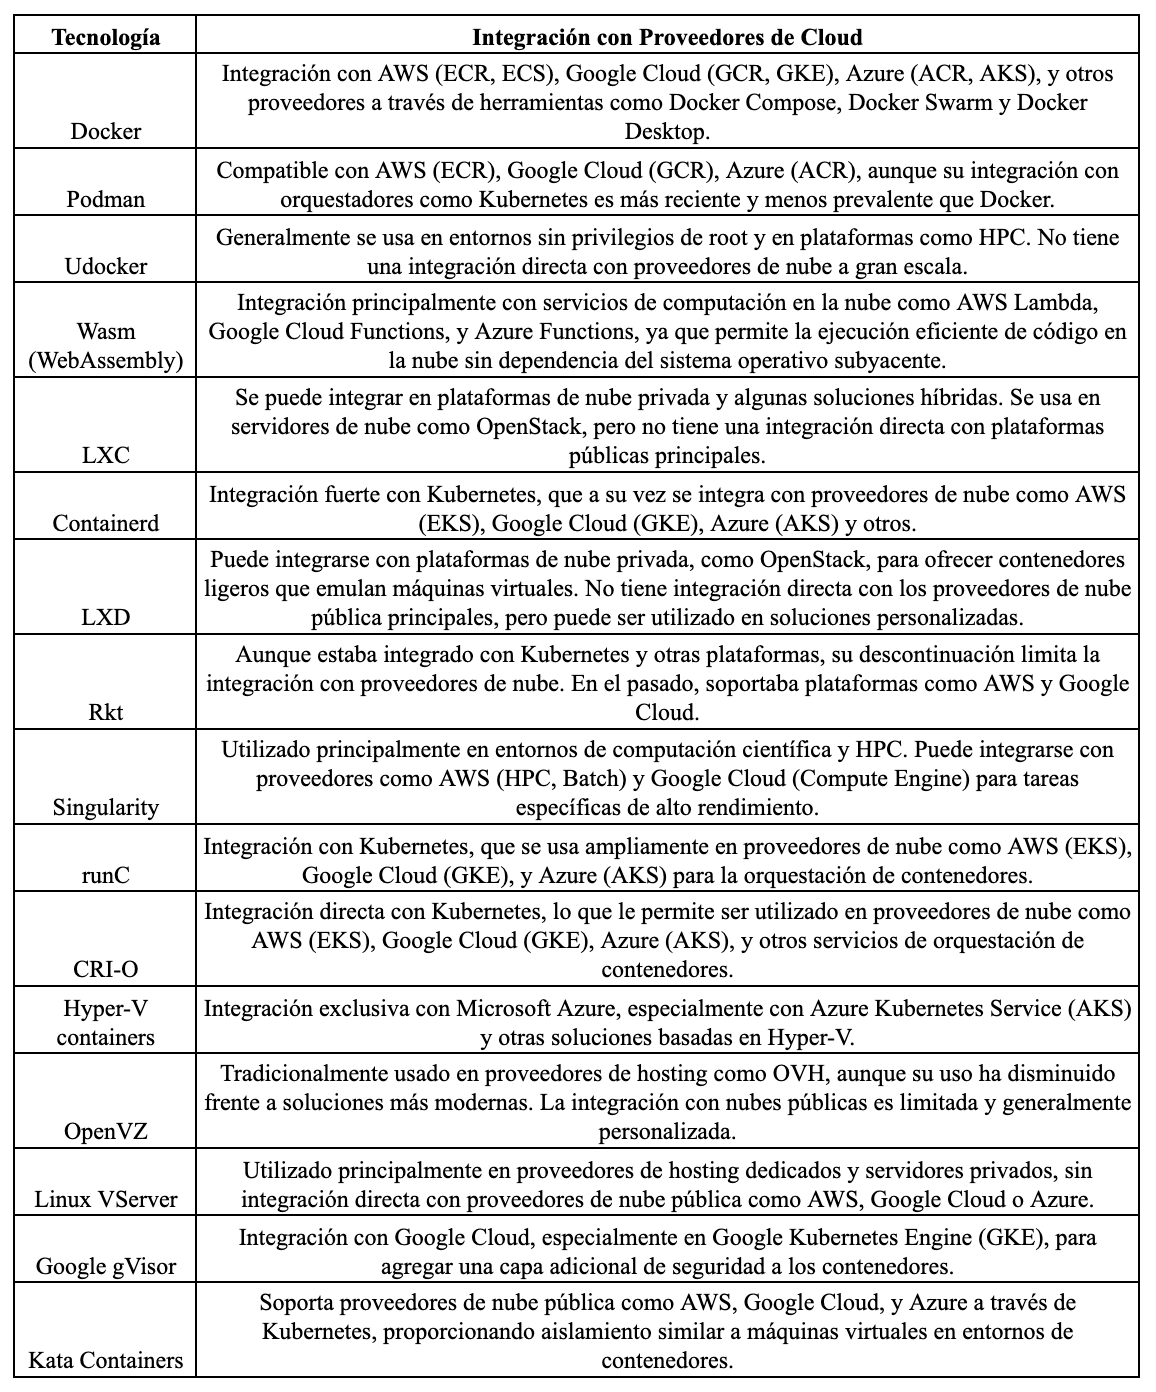
\includegraphics[width=\textwidth] {tablas-images/cp3/integracion-cloud.png}
    \caption{Integración cloud de cada VBC}\label{tab:tabla-integracion-cloud}
\end{table}

\clearpage
\section{Cuadrante Gartner}
Para visualizar el panorama de las tecnologias de contenerización en cuanto a su relevancia en la industria, se aplicó un cuadrante gartner, el cual mide dos dimensiones, Visión y Ejecución, es decir que tan buena proyeccion puede tener la tecnologia en el futuro y que tan bien se desempeña actualmente en el corto plazo.

\begin{table}[H]
\centering
\scriptsize
\setlength{\tabcolsep}{4pt}
\renewcommand{\arraystretch}{1.0}
\begin{tabular}{|p{0.3\textwidth}|c|c|p{0.25\textwidth}|}
\hline
\textbf{Tecnología} & \textbf{Visión (X)} & \textbf{Ejecución (Y)} & \textbf{Cuadrante} \\
\hline
Docker & 9 & 9 & Líderes \\
\hline
Containerd & 8 & 8 & Líderes \\
\hline
Podman & 8 & 7 & Retadores \\
\hline
CRI-O & 7 & 7 & Retadores \\
\hline
LXC & 6 & 6 & Jugadores de Nicho \\
\hline
LXD & 6 & 6 & Jugadores de Nicho \\
\hline
Udocker & 4 & 4 & Jugadores de Nicho \\
\hline
runC & 5 & 5 & Jugadores de Nicho \\
\hline
Rkt & 3 & 4 & Jugadores de Nicho \\
\hline
Singularity & 5 & 4 & Visionarios \\
\hline
Wasm & 9 & 5 & Visionarios \\
\hline
Google gVisor & 8 & 6 & Visionarios \\
\hline
Kata Containers & 7 & 6 & Visionarios \\
\hline
Firecracker & 8 & 6 & Visionarios \\
\hline
Sarus & 4 & 4 & Jugadores de Nicho \\
\hline
Hyper-V containers & 5 & 5 & Jugadores de Nicho \\
\hline
OpenVZ & 4 & 5 & Jugadores de Nicho \\
\hline
Linux VServer & 3 & 4 & Jugadores de Nicho \\
\hline
\end{tabular}
\caption{Tabla de medición para el cuadrante gartner}\label{tab:cuadrante-gartner}
\end{table}

Una vez hecha la tabla anterior, se pueden resumir los resultados en el diagrama~\ref{fig:tabla-cuadrante-gartner}, que representa el cuadrante Gartner. Se pueden ver 4 grandes grupos de tecnologías dependiendo de su nivel de visión y ejecución: Líderes, Retadores, Visionarios, Jugadores de nicho.
\begin{figure}[H]
    \centering
    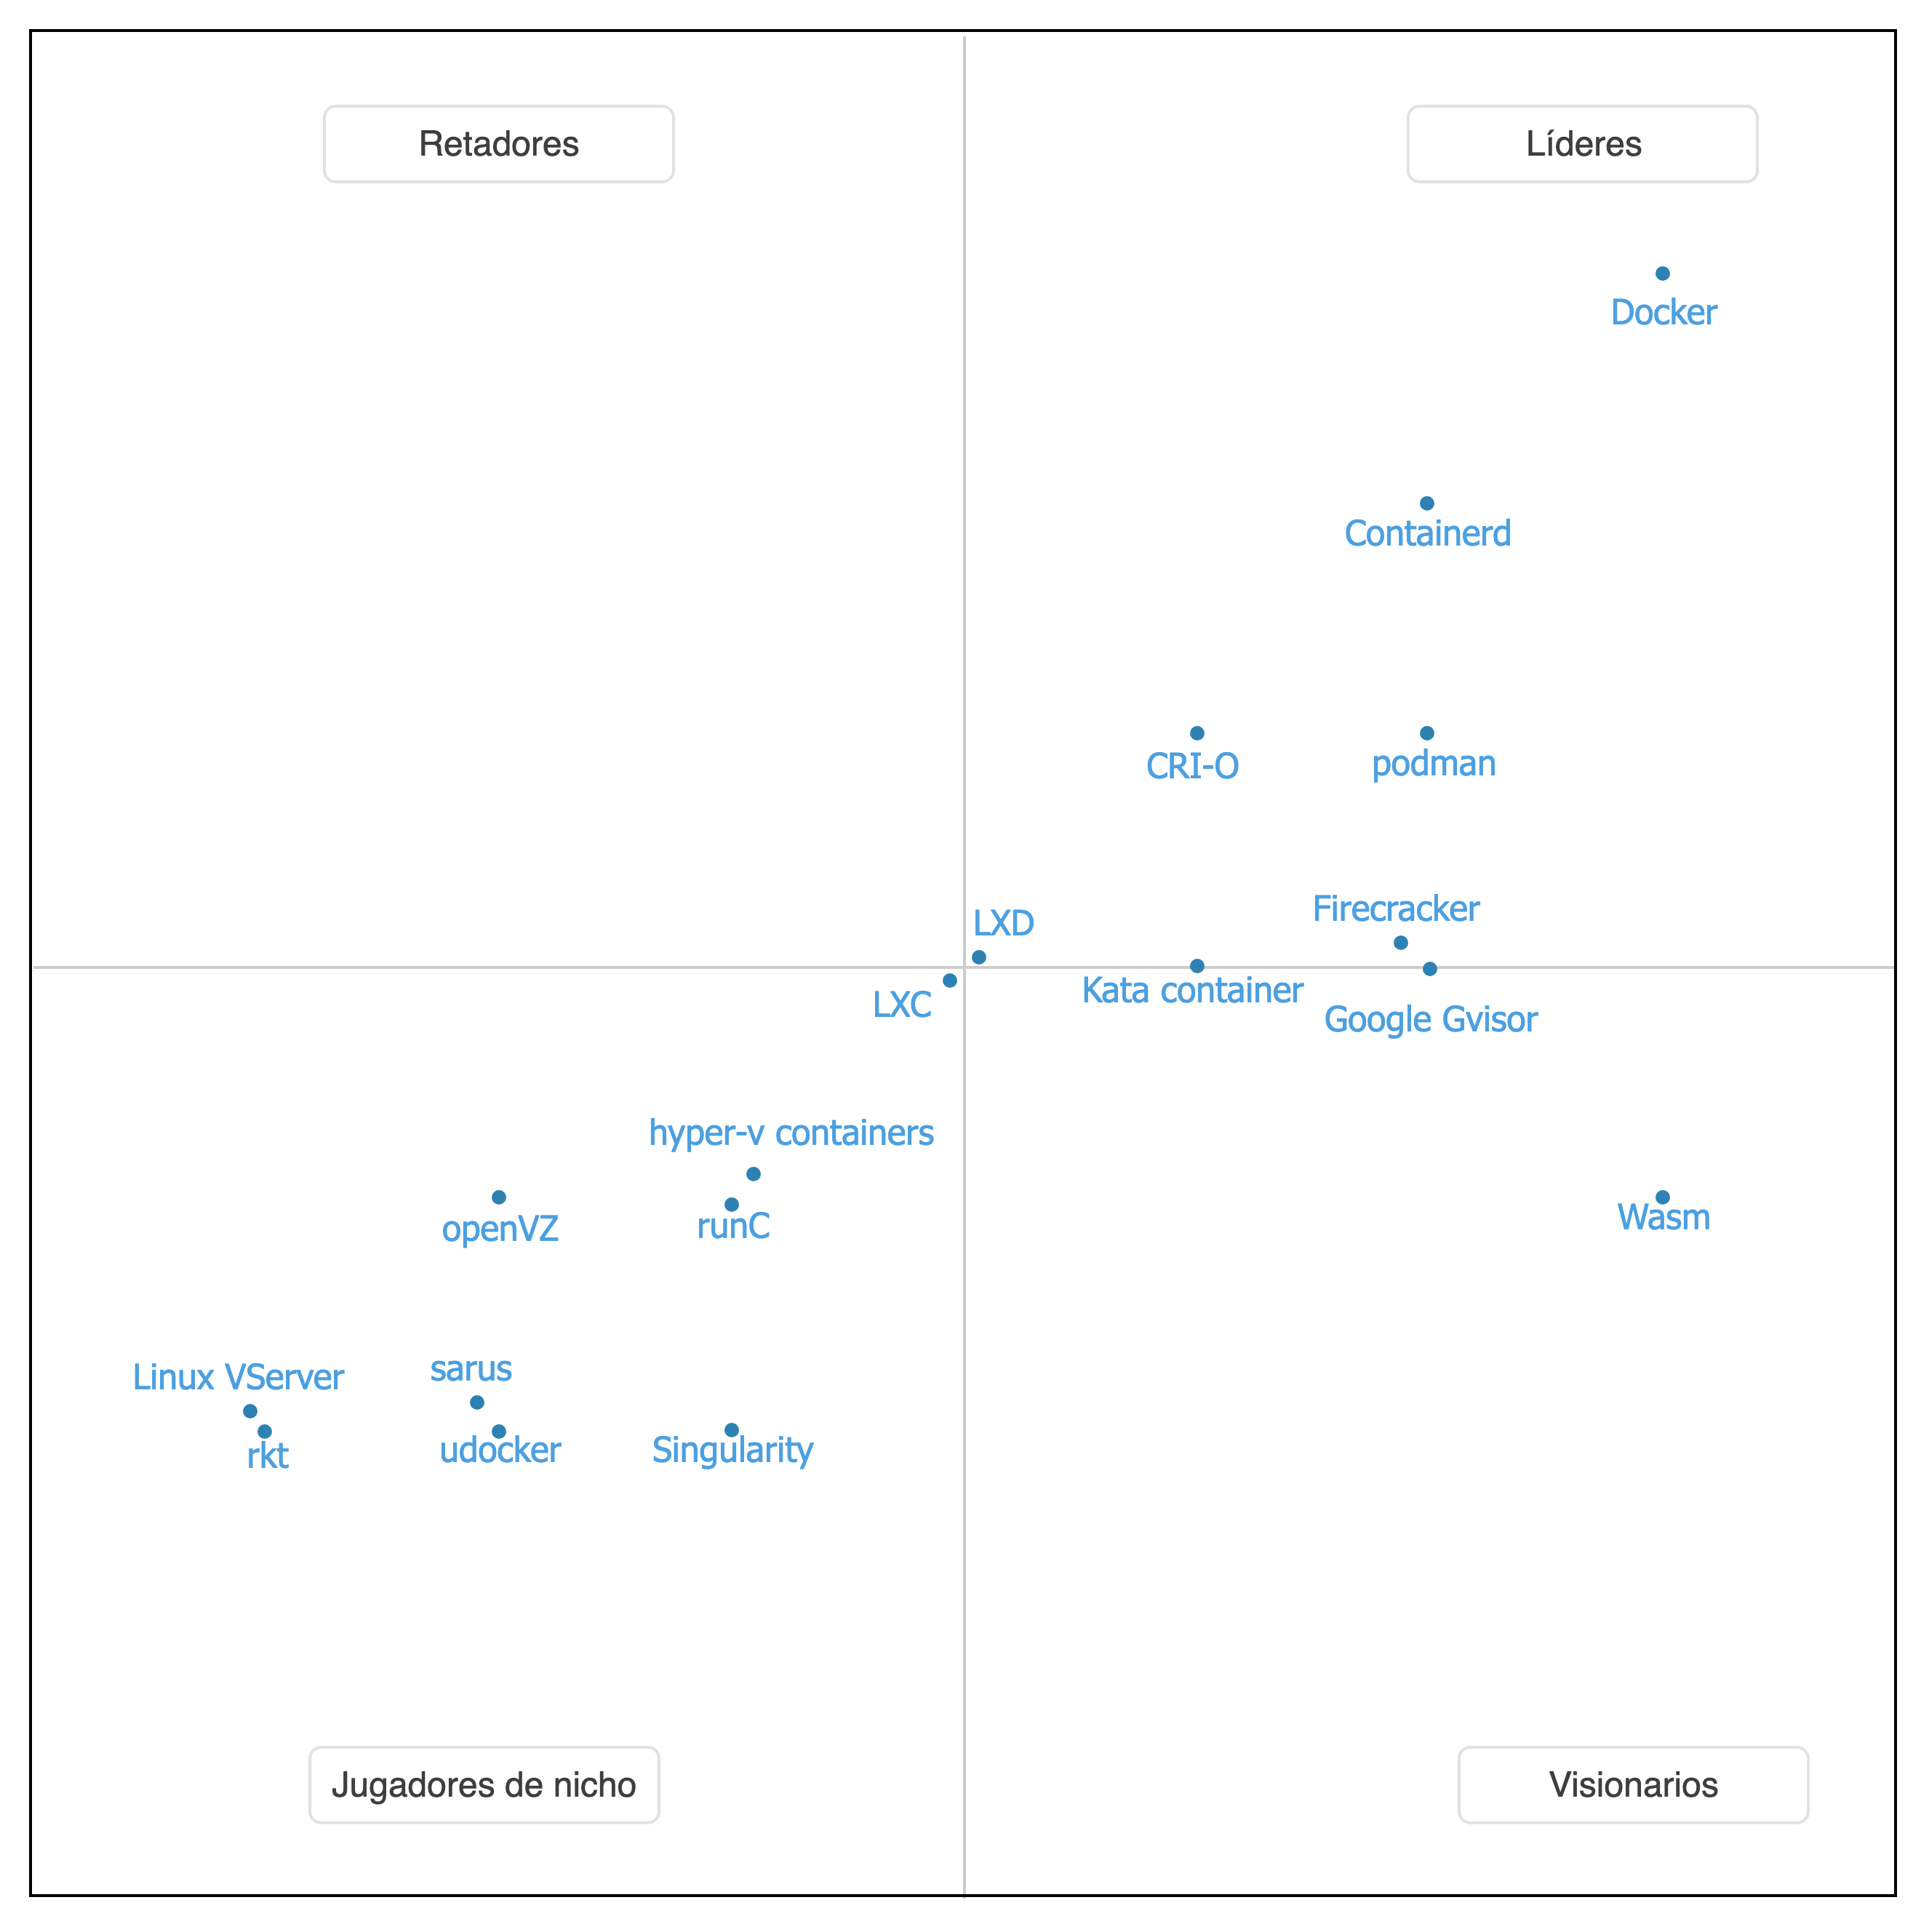
\includegraphics[width=\textwidth] {tablas-images/cp3/cuadrante-gartner.png}
    \caption{Cuadrante de Gartner de cada VBC}\label{fig:tabla-cuadrante-gartner}
\end{figure}

\section{Entornos de ejecución}
En la tabla~\ref{tab:entornos-ejecucion-vbc} se puede ver los sistemas operativos en los que se ejecutan estas tecnologias, se puede ver que la mayoria de estas estan diseñadas para sistemas linux, seguido de sistemas windows y por ultimo sistemas macOS, en cuyo caso las 2 unicas tecnologias que soportan este SO son ~\textit{Docker} y ~\textit{Podman}.
\begin{table}[H]
\centering
\scriptsize
\setlength{\tabcolsep}{3pt}
\renewcommand{\arraystretch}{1.1}
\begin{tabularx}{\textwidth}{|p{0.2\textwidth}|X|}
\hline
\textbf{Tecnología} & \textbf{Ambiente de Ejecución} \\
\hline
Docker & Sistemas Linux, Windows y macOS. Entornos de desarrollo, pruebas y producción, incluyendo la nube pública (\AWS, Google Cloud, Azure). \\
\hline
Podman & Sistemas Linux y macOS, con soporte experimental en Windows. Usado en entornos de desarrollo y producción sin necesidad de un daemon. \\
\hline
Udocker & Sistemas Linux, en entornos de computación de alto rendimiento (\HPC) y servidores compartidos, permitiendo ejecutar contenedores sin privilegios de root. \\
\hline
Wasm (WebAssembly) & Navegadores web (Chrome, Firefox, Safari, Edge). Ejecución en aplicaciones web y entornos de alto rendimiento sin dependencia del sistema operativo subyacente. \\
\hline
LXC & Sistemas Linux. Utilizado para crear contenedores ligeros que actúan como máquinas virtuales, con aplicaciones aisladas en servidores y plataformas de nube privada. \\
\hline
Containerd & Sistemas Linux y Windows. Usado en plataformas de orquestación como Kubernetes, y en infraestructuras de contenedores a gran escala. \\
\hline
LXD & Sistemas Linux. Virtualización ligera de contenedores como máquinas virtuales completas, ideal para servidores y plataformas de virtualización en la nube privada. \\
\hline
Rkt & Sistemas Linux. Anteriormente usado en entornos de orquestación de contenedores y en infraestructuras de nube privada. (Descontinuado actualmente). \\
\hline
Singularity & Sistemas Linux, especialmente en entornos de computación científica y \HPC. Portabilidad de aplicaciones científicas sin necesidad de privilegios de root. \\
\hline
runC & Sistemas Linux. Runtime ligero de contenedores compatible con los estándares de la Open Container Initiative (\OCI), utilizado por plataformas como Docker y Kubernetes. \\
\hline
CRI-O & Sistemas Linux. Integrado con Kubernetes para la gestión de contenedores en plataformas de orquestación en la nube y servidores locales. \\
\hline
Hyper-V containers & Sistemas Windows (Windows Server y Windows 10 con Hyper-V habilitado). Usado para contenedores con aislamiento mediante micro-VMs, ideal para entornos híbridos. \\
\hline
OpenVZ & Sistemas Linux. Virtualización a nivel de contenedor en proveedores de hosting para ofrecer entornos aislados. \\
\hline
Linux VServer & Sistemas Linux. Contenedores que funcionan como servidores virtuales, usados en entornos de hosting y administración de servidores de alta disponibilidad. \\
\hline
Google gVisor & Plataformas de nube, especialmente \GCP. Capa adicional de seguridad para contenedores en entornos multitenant. \\
\hline
Kata Containers & Sistemas Linux. Virtualización ligera con aislamiento similar a máquinas virtuales, utilizado en plataformas de contenedores en la nube y servidores donde se requiere seguridad. \\
\hline
Firecracker & Plataformas de computación en la nube, como \AWS. Diseñado para micro-VMs ultra ligeras y de alto rendimiento en entornos serverless. \\
\hline
Sarus & Sistemas Linux. Entornos de computación de alto rendimiento (\HPC) y clústeres de supercomputación, proporcionando portabilidad sin privilegios de root. \\
\hline
\end{tabularx}
\caption{Entornos de ejecución de cada VBC}\label{tab:entornos-ejecucion-vbc}
\end{table}

\section{Evaluación DOFA}
En el cuadro~\ref{tab:matriz-dofa} se define una matriz DOFA, especificando las debilidades, oportunidades, fortalezas y amenazas de las tecnologías VBC. Esto permite tener varios aspectos en cuenta a la hora de seleccionar una tecnología o realizar una implementación.
\begin{table}[H]
\centering
\scriptsize
\setlength{\tabcolsep}{4pt}
\renewcommand{\arraystretch}{1.2}
\begin{tabularx}{\textwidth}{|X|X|}
\hline
\multicolumn{1}{|c|}{\textbf{Fortalezas}} & \multicolumn{1}{c|}{\textbf{Oportunidades}} \\
\hline
\begin{minipage}[t]{\dimexpr\linewidth-8mm} % Reduced width for padding
\vspace{2pt}
\begin{itemize}
    \setlength\itemsep{0pt}
    \setlength\parskip{0pt}
    \setlength\parsep{0pt}
    \item \hspace{5mm} Herramientas como Kubernetes y Docker se actualizan constantemente, agregando nuevas funcionalidades y mejoras.
    \item \hspace{5mm} La \VBC\ es ampliamente utilizada en plataformas en la nube como AWS, Azure y Google Cloud.
    \item \hspace{5mm} Numerosos foros, grupos y organizaciones están dedicados a mejorar y desarrollar soluciones de contenerización.
    \item \hspace{5mm} Los contenedores pueden ejecutarse en múltiples entornos (local, nube, híbrido).
    \item \hspace{5mm} Permiten una mejor utilización de recursos en comparación con las máquinas virtuales tradicionales.
\end{itemize}
\vspace{2pt}
\end{minipage}
\hspace{4mm} % Right padding
&
\begin{minipage}[t]{\dimexpr\linewidth-8mm} % Reduced width for padding
\vspace{2pt}
\begin{itemize}
    \setlength\itemsep{0pt}
    \setlength\parskip{0pt}
    \setlength\parsep{0pt}
    \item \hspace{5mm} Los contenedores son ligeros y comparten el kernel del sistema operativo, reduciendo el consumo de recursos.
    \item \hspace{5mm} Una aplicación en contenedor puede ejecutarse en cualquier entorno compatible sin modificaciones.
    \item \hspace{5mm} Permiten implementar y gestionar aplicaciones de manera escalable y eficiente.
    \item \hspace{5mm} Los contenedores permiten que las aplicaciones se ejecuten de manera independiente, evitando conflictos entre ellas.
    \item \hspace{5mm} Herramientas como Docker Compose y Kubernetes facilitan la gestión automatizada de contenedores.
\end{itemize}
\vspace{2pt}
\end{minipage}
\hspace{4mm} % Right padding
\\
\hline
\multicolumn{1}{|c|}{\textbf{Debilidades}} & \multicolumn{1}{c|}{\textbf{Amenazas}} \\
\hline
\begin{minipage}[t]{\dimexpr\linewidth-8mm} % Reduced width for padding
\vspace{2pt}
\begin{itemize}
    \setlength\itemsep{0pt}
    \setlength\parskip{0pt}
    \setlength\parsep{0pt}
    \item \hspace{5mm} Los contenedores comparten el mismo núcleo del sistema operativo host, lo que podría permitir que una vulnerabilidad afecte a todos los contenedores.
    \item \hspace{5mm} A medida que crece la infraestructura, gestionar múltiples contenedores y sus redes se vuelve complejo.
    \item \hspace{5mm} A diferencia de las máquinas virtuales tradicionales, los contenedores son efímeros por diseño, lo que complica el manejo de datos persistentes.
    \item \hspace{5mm} No todos los sistemas y aplicaciones son compatibles de manera nativa con contenedores, lo que requiere configuraciones específicas.
    \item \hspace{5mm} La seguridad y rendimiento de los contenedores están directamente relacionados con el sistema operativo subyacente.
\end{itemize}
\vspace{2pt}
\end{minipage}
\hspace{4mm} % Right padding
&
\begin{minipage}[t]{\dimexpr\linewidth-8mm} % Reduced width for padding
\vspace{2pt}
\begin{itemize}
    \setlength\itemsep{0pt}
    \setlength\parskip{0pt}
    \setlength\parsep{0pt}
    \item \hspace{5mm} Si no se aplican buenas prácticas, los contenedores pueden ser vulnerables a ataques.
    \item \hspace{5mm} El uso de soluciones propietarias como \AWS\ o Azure puede generar dependencia tecnológica.
    \item \hspace{5mm} Las tecnologías de contenerización evolucionan rápidamente, lo que puede dejar obsoletas algunas soluciones.
    \item \hspace{5mm} Un mal diseño puede llevar a un consumo ineficiente de recursos.
    \item \hspace{5mm} Aunque existen buenas prácticas, no hay una regulación estándar única para la gestión de contenedores.
\end{itemize}
\vspace{2pt}
\end{minipage}
\hspace{4mm} % Right padding
\\
\hline
\end{tabularx}
\caption{Tabla de matriz DOFA para el cuadrante gartner}\label{tab:matriz-dofa}
\end{table}
\begin{table}[H]
\centering
\rowcolors{2}{gray!10}{white}
\begin{tabularx}{\textwidth}{>{\raggedright\arraybackslash}X >{\raggedright\arraybackslash}X}
\rowcolor{gray!30}
\textbf{Tecnología} & \textbf{Enlace a la Documentación} \\

Docker & \href{https://docs.docker.com/}{link} \\
Podman & \href{https://podman.io/docs}{link} \\
Udocker & \href{https://github.com/indigo-dc/udocker}{link} \\
Wasm (WebAssembly) & \href{https://webassembly.org/docs/faq/}{link} \\
LXC & \href{https://linuxcontainers.org/incus/docs/main/}{link} \\
Containerd & \href{https://containerd.io/docs/}{link} \\
LXD & \href{https://linuxcontainers.org/incus/docs/main/}{link} \\
Rkt & \href{https://github.com/rkt/rkt}{link} \\
Singularity & \href{https://docs.sylabs.io/guides/4.3/user-guide/}{link} \\
runC & \href{https://github.com/opencontainers/runc}{link} \\
CRI-O & \href{https://github.com/cri-o/cri-o}{link} \\
Hyper-V containers & \href{https://docs.microsoft.com/en-us/virtualization/windowscontainers/}{link} \\
OpenVZ & \href{https://openvz.org/}{link} \\
Linux VServer & \href{http://linux-vserver.org/Documentation}{link} \\
Google gVisor & \href{https://gvisor.dev/docs/}{link} \\
Kata Containers & \href{https://katacontainers.io/docs/}{link} \\
Firecracker & \href{https://firecracker-microvm.github.io/}{link} \\
Sarus & \href{https://github.com/eth-cscs/sarus}{link} \\

\end{tabularx}
\caption{Enlaces a la documentación de tecnologías de contenerización}
\end{table}
\ChapterImageStar[cap:benchmarking]{Benchmarking}{./images/fondo.png}\label{cap:benchmarking}

\mbox{}\\
\section{Descripción del escenario de pruebas}\label{sec:escenario-pruebas}
\noindent
Las características del entorno de prueba incluyeron el uso de una máquina con especificaciones técnicas homogéneas, propendiendo  porque las diferencias en rendimiento se debieran exclusivamente a las tecnologías evaluadas y no a variaciones en el hardware o la configuración del sistema operativo, las características del entorno de prueba se detallan a continuación:\\ \\
\noindent
En la Figura~\ref{fig:CPU-benchmarking} se presenta la información correspondiente al procesador utilizado en el entorno de \textit{benchmarking}, obtenida mediante el comando \texttt{lscpu}. En ella se evidencia que la arquitectura de la \CPU\ es x86\_64, con soporte para operaciones en 32 y 64 bits, y direcciones de memoria de 39 bits físicos y 48 bits virtuales. Asimismo, se observa que el procesador corresponde a un Intel Core i7-5600U \CPU\ de 2.60GHz, perteneciente a la familia de procesadores de Intel, lo cual permite contar con un recurso de hardware adecuado para la ejecución de pruebas de rendimiento bajo condiciones controladas.
\begin{figure}[H]
    \centering
    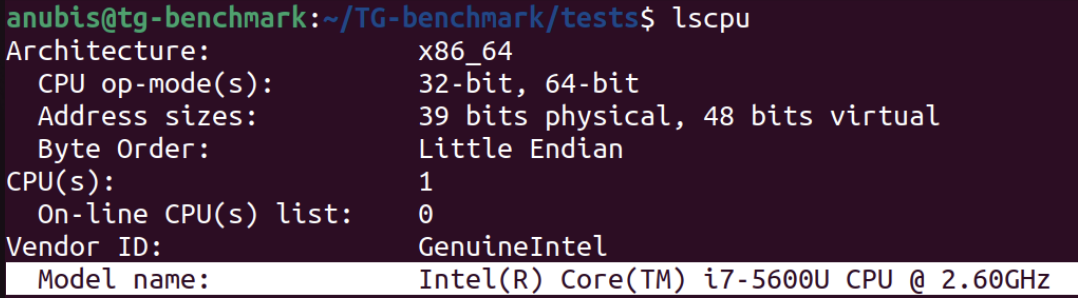
\includegraphics[width=\textwidth,height=0.85\textheight,keepaspectratio]{apendices/ENV-BENCH/CPU.png}
    \caption{CPU del entorno de \textit{benchmarking}}\label{fig:CPU-benchmarking}
\end{figure}

\noindent
En la Figura~\ref{fig:RAM-benchmarking} se muestra el estado de la memoria principal del entorno de \textit{benchmarking}, obtenido mediante el comando \texttt{free -h}. Se observa que el sistema cuenta con un total de 1.9 GiB de \RAM, de los cuales aproximadamente 572 MiB se encuentran en uso, mientras que 956 MiB permanecen libres. Adicionalmente, se dispone de 596 MiB utilizados por el sistema como memoria intermedia y de caché, dejando un total de 1.3 GiB disponibles para ejecución de procesos.
\begin{figure}[H]
    \centering
    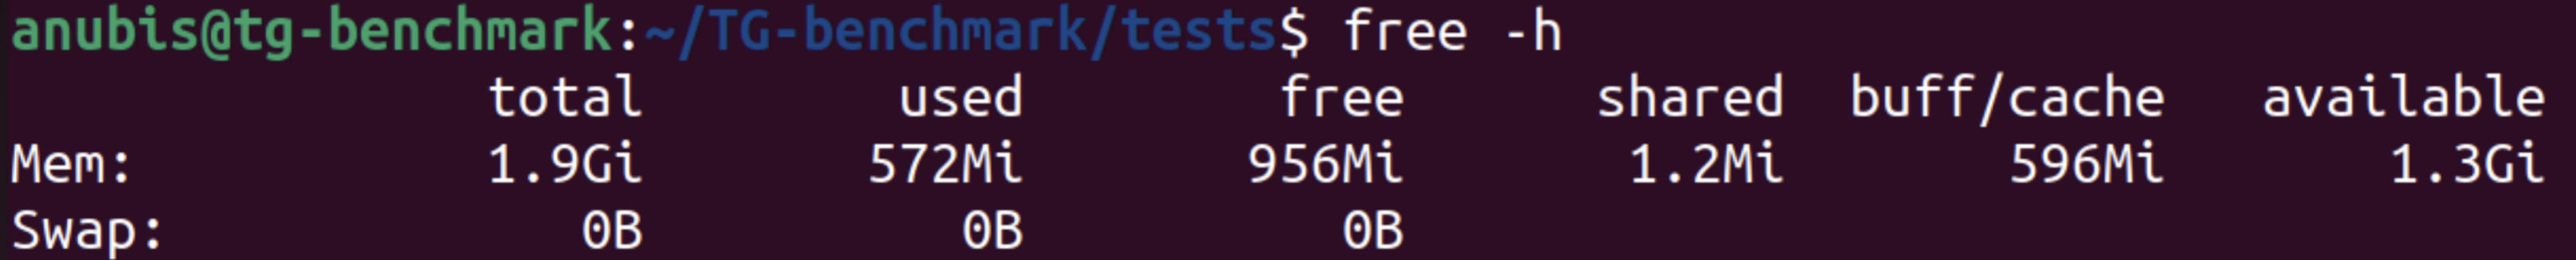
\includegraphics[width=\textwidth,height=0.85\textheight,keepaspectratio]{apendices/ENV-BENCH/RAM.png}
    \caption{RAM del entorno de \textit{benchmarking}}\label{fig:RAM-benchmarking}
\end{figure}
\noindent
En la Figura~\ref{fig:DISK-benchmarking} se presenta la información del sistema de archivos correspondiente al disco del entorno de \textit{benchmarking}, obtenida mediante el comando \texttt{df -Th}. El resultado muestra que el volumen principal está montado sobre el directorio raíz /, con un sistema de archivos ext4, una capacidad total de 14 GB, de los cuales 7.2 GB se encuentran en uso y 5.3 GB permanecen disponibles, lo que representa un 58\% de ocupación. Estos datos permiten evidenciar las características de almacenamiento del entorno, así como su disponibilidad para la ejecución de las pruebas experimentales sin limitaciones significativas de espacio.
\begin{figure}[H]
    \centering
    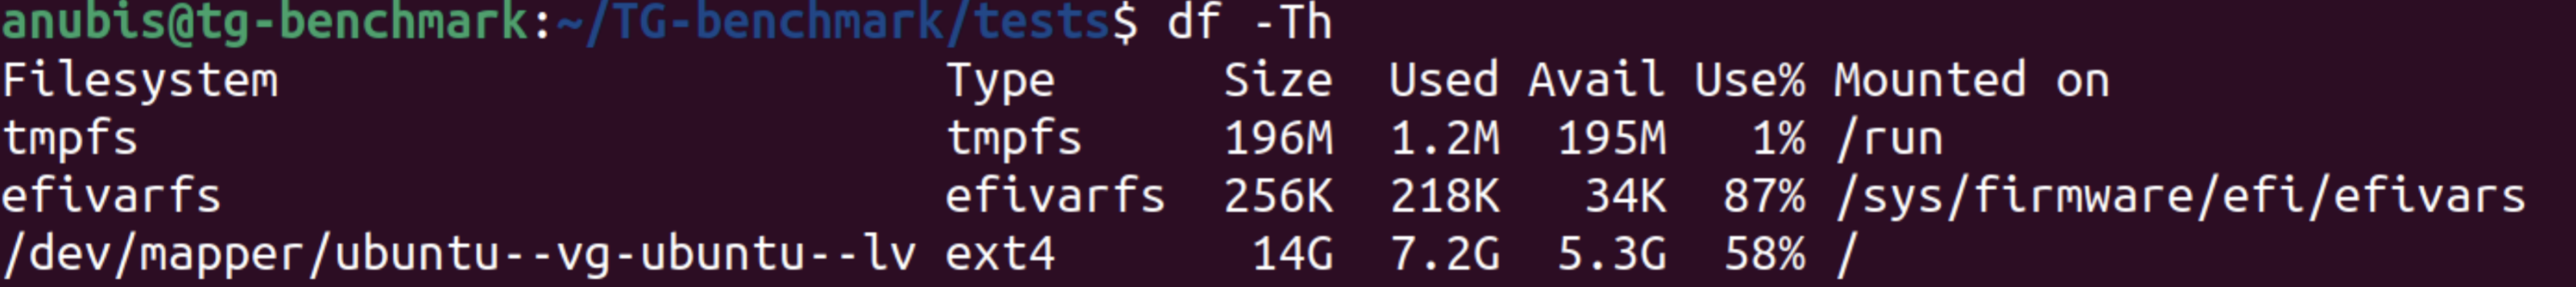
\includegraphics[width=\textwidth,height=0.85\textheight,keepaspectratio]{apendices/ENV-BENCH/DISCO.png}
    \caption{Disco del entorno de \textit{benchmarking}}\label{fig:DISK-benchmarking}
\end{figure}
\noindent
En la Figura~\ref{fig:OS-benchmarking} se presenta la información del sistema operativo empleado en el entorno de \textit{benchmarking}, obtenida mediante el comando \texttt{lsb\_release -a}. El resultado indica que se utiliza la distribución Ubuntu 24.04.2 LTS, cuyo nombre en clave es noble. Esta versión corresponde a una edición de soporte extendido (\textit{Long Term Support}), lo que ofrece estabilidad, actualizaciones de seguridad y mantenimiento a largo plazo. La elección de este sistema operativo resulta adecuada para la ejecución de pruebas experimentales, dado que proporciona un entorno ampliamente soportado en la comunidad de software libre.
\begin{figure}[H]
    \centering
    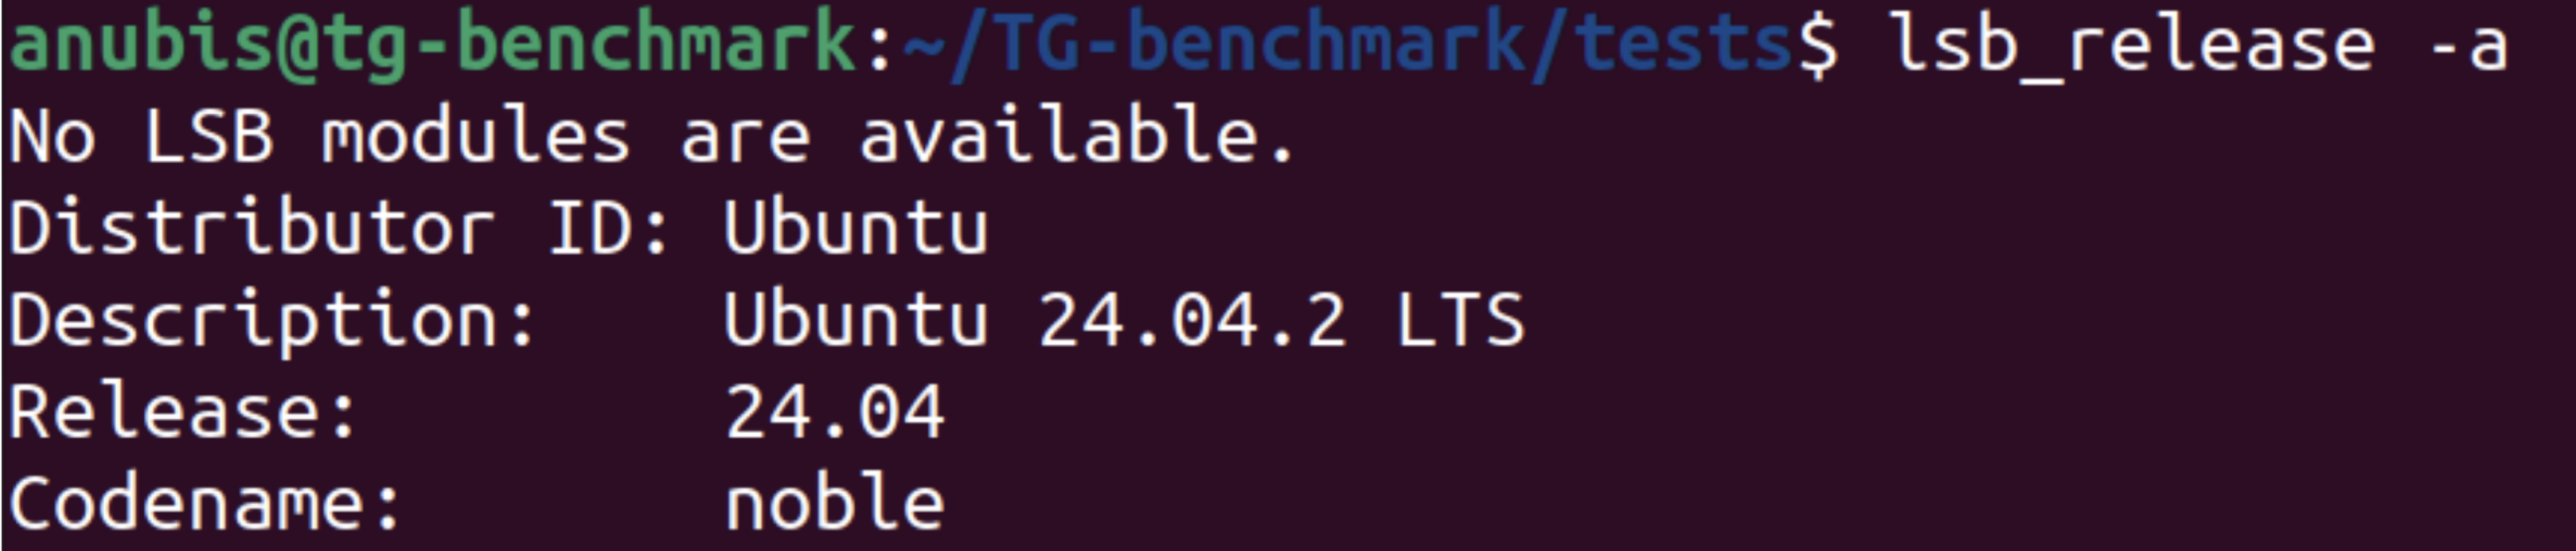
\includegraphics[width=\textwidth,height=0.85\textheight,keepaspectratio]{apendices/ENV-BENCH/OS.png}
    \caption{Sistema operativo del entorno de \textit{benchmarking}}\label{fig:OS-benchmarking}
\end{figure}
En la Figura~\ref{fig:INTERFACES-benchmarking} se muestra la configuración de las interfaces de red del entorno de benchmarking, obtenida mediante el comando \texttt{ip a}. Se identifican varias interfaces activas, entre ellas la \texttt{lo} (loopback) utilizada para la comunicación interna del sistema, así como \texttt{enp0s3} y \texttt{enp0s8}, ambas en estado operativo (UP) y con direcciones IPv4 asignadas en las subredes 10.0.2.0/24 y 192.168.0.0/24, respectivamente, además de direcciones IPv6 asociadas. También se observan interfaces virtuales, como \texttt{lxcbro} y \texttt{lxdbro}, que si bien aparecen en estado inactivo (DOWN), evidencian la presencia de configuraciones de red orientadas a entornos virtualizados. Esta información permite caracterizar la conectividad del sistema y su capacidad de interacción con diferentes redes dentro del proceso de evaluación de rendimiento.
\begin{figure}[H]
    \centering
    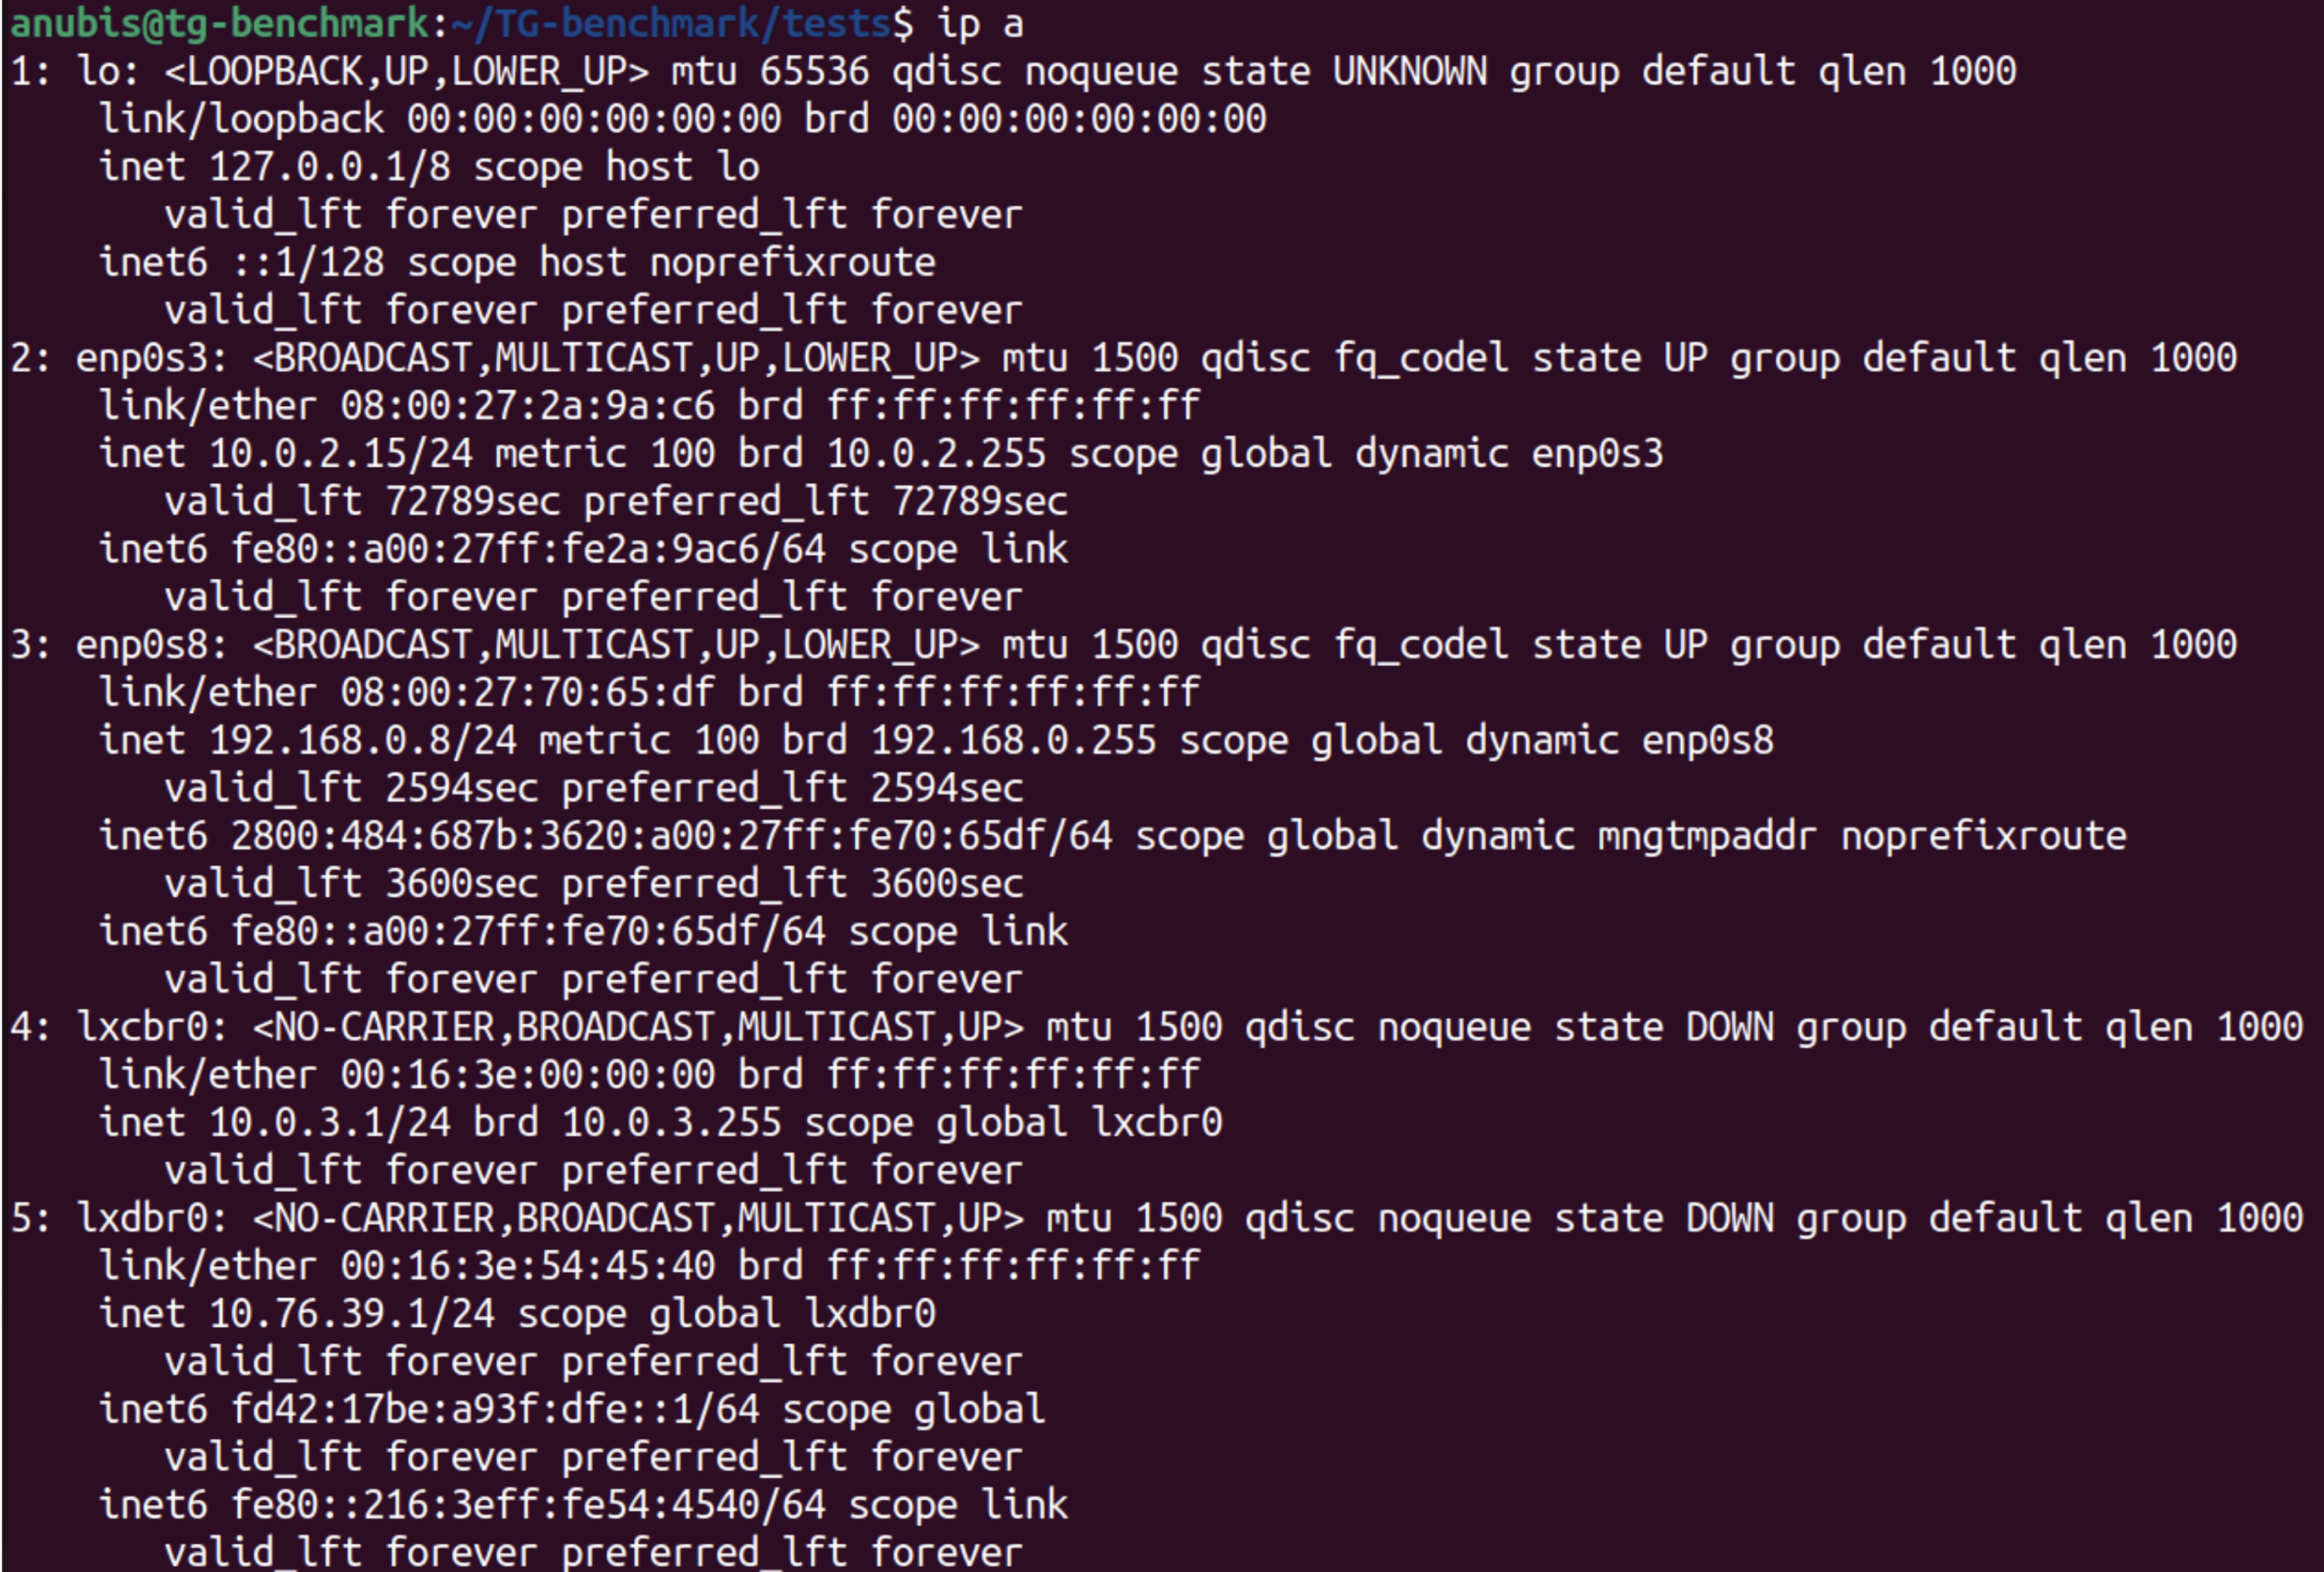
\includegraphics[width=\textwidth,height=0.85\textheight,keepaspectratio]{apendices/ENV-BENCH/interfaces.png}
    \caption{Interfaces de red del entorno de \textit{benchmarking}}\label{fig:INTERFACES-benchmarking}
\end{figure}

\section{Definición de las pruebas}
\noindent
Para evaluar el rendimiento de distintas tecnologías de contenerización —específicamente Docker, Podman, LXC, LXD y Containerd— se diseñó un conjunto de pruebas orientadas a medir aspectos clave del desempeño en entornos controlados. Las pruebas incluyeron el consumo de CPU y memoria RAM, el tiempo de arranque de los contenedores, el \textit{throughput} de red y la latencia de acceso a disco. 
Con el objetivo de facilitar la repetibilidad y objetividad de los resultados, se desarrollaron scripts en \textit{Bash} que automatizan la ejecución de cada métrica en condiciones homogéneas. Estas pruebas permiten comparar las tecnologías evaluadas bajo criterios cuantificables y facilitar un análisis técnico de sus capacidades en escenarios reales de uso.

\section{Construcción de las pruebas}
\noindent
La construcción de las pruebas se llevó a cabo mediante el desarrollo de scripts automatizados en \textit{Bash}, diseñados para ejecutarse de forma uniforme sobre cada tecnología de contenerización evaluada. Cada script fue responsable de iniciar contenedores, ejecutar cargas de trabajo específicas y recolectar métricas de rendimiento relevantes.
Para medir el consumo de \CPU\ y memoria \RAM, se utilizó \texttt{pidstat}, una utilidad que permite la medición del consumo de recursos. El tiempo de arranque se determinó midiendo el intervalo entre la orden de inicio del contenedor y el momento en que estuvo completamente operativo. 
Para evaluar el \textit{throughput} de red se emplearon herramientas como \texttt{iperf}, mientras que la latencia de disco fue medida utilizando \texttt{fio}. Todas las pruebas fueron ejecutadas múltiples veces para reducir el impacto de variaciones puntuales y asegurar la confiabilidad de los resultados. Los scripts fueron programados para ejecutarse 10 veces; al final se extrae un promedio y este constituye el puntaje final de la tecnología de contenerización en cuestión.
En el repositorio \underline{\href{https://github.com/Anubis-1001/benchmark-tecnologias-de-contenerizacion} {\texttt{ GitHub benchmarking}}} se pueden encontrar los scripts resultantes de este proceso.

\section{Resultados de las pruebas}\label{sec:resultados-pruebas}
\noindent
Los resultados obtenidos a partir de las pruebas evidencian diferencias significativas en el rendimiento entre las tecnologías de contenerización evaluadas. Estos se pueden consultar en el archivo de Excel \underline{\href{https://docs.google.com/spreadsheets/d/1Ce37Sm3Swyfa88Ur1yQbLarq_D86obUIAGGJocgQbUE/edit?usp=sharing} {\texttt{benchmarking\_tecnologias}}}.
En términos de consumo de \CPU, Docker y Containerd presentan las mejores métricas; en consumo de memoria \RAM, LXC y LXD mostraron un mejor uso de los recursos. En cuanto al tiempo de arranque, Containerd destacó por su velocidad, seguido de cerca por Docker, mientras que LXC presentó un arranque considerablemente más lento en comparación con las demás tecnologías.
Para el \textit{throughput} de red, todas las tecnologías mostraron un desempeño comparable, siendo LXC el más destacado; no obstante, Podman quedó muy por debajo en esta métrica. Finalmente, en la medición de latencia de disco, LXD y Containerd obtuvieron los mejores resultados, lo que sugiere una gestión de E/S más directa y liviana.
Estos resultados permiten establecer un panorama claro de fortalezas y debilidades de cada solución, según el tipo de carga o entorno de ejecución esperado.

\section{Métricas de rendimiento}
\noindent
De la ejecución de las pruebas se obtuvieron las siguientes métricas de rendimiento: \\

\noindent
La figura~\ref{fig:tabla-metricas-cpu} muestra una comparación del porcentaje de uso de \CPU. Este análisis permite observar el nivel de utilización del procesador al ejecutar cargas de trabajo bajo entornos como Docker, Containerd, LXD, LXC y Podman. Los resultados tienen contrastes significativos entre las tecnologías, destacando aquellas que logran un mayor aprovechamiento del recurso de CPU frente a otras con un desempeño relativamente inferior.
\begin{figure}[H]
    \centering
    \includegraphics[width=\textwidth] {tablas-images/cp4/cpu.png}
    \caption{Métricas de uso de CPU}\label{fig:tabla-metricas-cpu}
\end{figure}

\noindent
La figura~\ref{fig:tabla-metricas-ram} presenta una comparación del porcentaje de uso de memoria \RAM para el conjunto de tecnologías seleccionado. Este análisis permite evaluar el consumo de recursos de cada solución, considerando que un menor uso de memoria representa una ventaja en términos de escalabilidad y rendimiento en entornos de alta demanda. Los resultados muestran valores muy cercanos entre las tecnologías evaluadas, lo que sugiere un comportamiento homogéneo en este aspecto, aunque con ligeras variaciones que pueden influir en la elección según el contexto de uso.
\begin{figure}[H]
    \centering
    \includegraphics[width=\textwidth] {tablas-images/cp4/ram.png}
    \caption{Métricas de uso de RAM}\label{fig:tabla-metricas-ram}
\end{figure}

\noindent
La figura~\ref{fig:tabla-metricas-io} muestra las métricas de latencia en operaciones de entrada/salida (E/S) para el conjunto de tecnologías seleccionado, expresadas en microsegundos. Este indicador es fundamental para evaluar el rendimiento de aplicaciones que dependen de un acceso rápido a datos y procesos intensivos en E/S. Los resultados reflejan diferencias significativas entre las tecnologías, evidenciando desde valores muy bajos, como en LXD, hasta tiempos de respuesta considerablemente altos, como en Podman. Este contraste permite identificar cuáles soluciones resultan más adecuadas en escenarios donde el manejo de datos es un factor crítico.
\begin{figure}[H]
    \centering
    \includegraphics[width=\textwidth] {tablas-images/cp4/io.png}
    \caption{Métricas de entrada/salida}\label{fig:tabla-metricas-io}
\end{figure}

\noindent
La figura~\ref{fig:tabla-metricas-throughput} presenta una comparación de las métricas de throughput (rendimiento de transferencia de datos) para el conjunto de tecnologías seleccionado, expresadas en Gbits por segundo. Este parámetro resulta clave para evaluar la capacidad de cada tecnología en la transmisión de información a través de la red, lo cual impacta directamente en el desempeño de aplicaciones distribuidas y servicios en la nube. Los resultados muestran un rendimiento consistente en tecnologías como LXC, LXD, Docker y Containerd, mientras que Podman evidencia un throughput significativamente más bajo, lo que resalta contrastes importantes en términos de consumo de red
\begin{figure}[H]
    \centering
    \includegraphics[width=\textwidth] {tablas-images/cp4/THROUGHTPUT.png}
    \caption{Métricas de throughput}\label{fig:tabla-metricas-throughput}
\end{figure}

\section{Análisis de los resultados}
\noindent
Los resultados obtenidos a partir de las pruebas permiten identificar comportamientos diferenciados entre las tecnologías de contenerización evaluadas. Containerd se posiciona como una de las soluciones más equilibradas, con excelente tiempo de arranque, bajo uso de CPU y buena latencia de disco, lo que lo hace ideal para entornos de bajos recursos.
LXC mostró consistentemente el menor consumo de recursos y alto rendimiento en red, lo que lo convierte en una opción adecuada para sistemas embebidos o despliegues que requieren un uso mínimo de \textit{overhead}. 
Por otro lado, Docker ofreció un rendimiento aceptable, pero con mayores niveles de consumo de CPU y latencia de disco, compensados por su madurez y ecosistema. 
LXD, al estar basado en LXC, heredó parte de sus beneficios, especialmente en uso de red, aunque con un ligero incremento en el tiempo de arranque.
En contraste, Podman, si bien ofrece un buen uso de CPU y memoria, presentó resultados considerablemente bajos en el \textit{throughput} de red y alta latencia de disco, lo cual podría limitar su aplicación en cargas sensibles a E/S o comunicación intensiva.

\vspace{0.5em}

\noindent En resumen, la elección de la tecnología de contenerización debe considerar el caso de uso específico: Containerd y LXC sobresalen por su bajo consumo de recursos; Docker y LXD ofrecen robustez y facilidad de integración; mientras que Podman puede ser más adecuado para entornos que prioricen la seguridad y compatibilidad con el modelo sin \textit{daemon}, siempre que el rendimiento de red o disco no sea crítico.

\ChapterImageStar[cap:dar]{Análisis de Decisiones y Resolución}{./images/fondo.png}\label{cap:dar}
\mbox{}\\
\section{Metodología de evaluación}
\noindent
La metodología de evaluación que se aplicó para la elección de la tecnología de \VBC fue \textit{Decision, analysis and resolution} (\DAR) de CMMI \citep{CMMIInstitute2010}. Esta metodología permitió evaluar las necesidades del grupo \GRID\ a través de un proceso estructurado que consideró múltiples alternativas, criterios de evaluación bien definidos y un análisis comparativo. En este caso, se analizaron las tecnologías \VBC\ encontradas en la revisión literaria, aplicando criterios como el tipo de licencia, la compatibilidad con herramientas de orquestación, el rendimiento entre otros. Así, el uso de \DAR\ no solo busca aportar transparencia al proceso, sino también trazabilidad y justificación técnica frente a una decisión para la arquitectura de infraestructura basada en contenedores.
El proceso de evaluación quedó registrado en un vídeo explicativo disponible en \href{https://youtu.be/xOmuQs2RX2c}{link}.

\section{Resultados de la evaluación}
\noindent
La tabla~\ref{tab:tabla-dar} presenta la aplicación de la metodología \DAR\ al proceso de selección de tecnologías de \VBC\. Este enfoque permitió evaluar de manera estructurada diversos criterios como el tipo de licencia, compatibilidad con orquestadores, soporte para redes y volúmenes, documentación disponible, consumo de recursos y costo de implementación en entornos productivos. Al asignar valores ponderados a cada aspecto, el análisis facilita la comparación objetiva entre múltiples alternativas, proporcionando un marco de referencia sólido para identificar la solución más adecuada según las necesidades técnicas, operativas y estratégicas de un proyecto.
\begin{table}[H]
    \centering
    \includegraphics[width=\textwidth] {tablas-images/cp5/DAR.png}
    \caption{Análisis de Decisiones y Resolución (DAR) aplicado a la selección de VBC}\label{tab:tabla-dar}
\end{table}

\section{Criterios de evaluación}

\subsection{VBC (¿Es una tecnología basada en contenedores?)}
\noindent
Este criterio define si la tecnología analizada entra dentro de la categoría de virtualización basada en contenedores, lo cual es el punto de partida para que pueda ser considerada en el análisis. Se evalúa como Sí (SI) o No (NO).

\subsection{Tipo de licencia}
\noindent
Se analiza el tipo de licencia bajo la cual se distribuye la tecnología, ya que esto afecta su adopción en proyectos académicos o comerciales. Las licencias permisivas (como Apache 2.0 o BSD) permiten mayor libertad de uso y modificación, mientras que licencias restrictivas (como AGPL o licencias propietarias) imponen ciertas limitaciones legales o técnicas.

\subsection{Posibilidad de orquestación}\label{sec:posibilidad-orquestacion}
\noindent
Se refiere a la capacidad de la tecnología para integrarse con herramientas de orquestación como Kubernetes, Docker Swarm o Apache mesos, lo cual es clave para la gestión automatizada de contenedores a gran escala. Una mayor puntuación indica mejor compatibilidad y soporte para estas herramientas.

\subsection{Compatibilidad con imágenes de Docker Hub}
\noindent
Evalúa si la tecnología puede ejecutar imágenes obtenidas directamente desde Docker Hub, el repositorio más utilizado para contenedores. Esto facilita la reutilización de contenedores existentes y la integración con flujos de trabajo ya establecidos.

\subsection{Soporte para redes personalizadas}
\noindent
Determina si la tecnología permite la creación y gestión de redes personalizadas entre contenedores. Este aspecto es fundamental en arquitecturas distribuidas, donde la comunicación entre servicios debe configurarse de forma segura.

\subsection{Persistencia de datos / volúmenes}
\noindent
Analiza si la solución permite la persistencia de datos, es decir, que los datos generados dentro de un contenedor puedan mantenerse incluso después de reiniciarlo o eliminarlo. Esto se logra mediante el uso de volúmenes o sistemas de almacenamiento externos.

\subsection{Documentación}
\noindent
Se valora la calidad, profundidad y accesibilidad de la documentación oficial. Una buena documentación facilita el aprendizaje, la resolución de problemas y la implementación de la tecnología.

\subsection{Soporte al proyecto}
\noindent
Considera el respaldo que tiene la tecnología por parte de la comunidad, empresas o fundaciones (como CNCF o Red Hat). Esto incluye mantenimiento activo, actualizaciones regulares, y foros o canales de ayuda disponibles.

\subsection{Popularidad}
\noindent
Este criterio mide la adopción y visibilidad de la tecnología, lo cual puede reflejar su madurez, confianza del mercado y disponibilidad de talento capacitado. Se puede estimar por métricas como el número de estrellas en GitHub.

\subsection{Consumo de recursos}
\noindent
Evalúa el nivel de consumo de recursos respecto al uso de CPU, memoria y almacenamiento. Se valora según lo que mencionan las organizaciones responsables en este aspecto.

\subsection{Compatibilidad de orquestación}
\noindent
Difiere levemente del punto~\ref{sec:posibilidad-orquestacion}, ya que aquí se mide qué tan bien se integra con los orquestadores, considerando estabilidad, plugins nativos y experiencia de uso. Un puntaje alto indica integración fluida y confiable.

\subsection{Costo de implementación y operación en ambientes productivos}
\noindent
Este criterio analiza los costos asociados a poner en marcha la tecnología en un entorno real. Incluye licencias, infraestructura, tiempo de configuración y mantenimiento. Una puntuación alta significa bajo costo o costo nulo, lo cual es ideal para instituciones académicas o proyectos con presupuesto limitado.
\section{Tecnología VBC adecuada}
\noindent
Del análisis comparativo realizado, \textbf{Containerd} se posiciona como la tecnología de virtualización basada en contenedores con mejor desempeño general. Destaca por su alta compatibilidad con Docker Hub, soporte para redes y volúmenes, excelente integración con orquestadores como Kubernetes, y una licencia permisiva~\footnote{Una licencia permisiva en tecnología es un tipo de licencia de software de código abierto que otorga a los usuarios una amplia libertad para usar, modificar y redistribuir el software, incluso en proyectos propietarios o comerciales, siempre que se cumplan requisitos mínimos, como mantener los avisos de copyright y la atribución original.}. que facilita su adopción. Además, cuenta con una amplia documentación y un respaldo activo de la comunidad. Estas características hacen de Containerd la opción adecuada, según el análisis \DAR, para ser implementada en ambientes productivos del grupo de investigación \GRID.
\clearpage
\section{Análisis \DAR\ del motor de Kubernetes}
\noindent
El análisis presentado en la figura~\ref{tab:tabla-dar-k8s} aplica la metodología \DAR\ al proceso de selección del motor de Kubernetes más adecuado para entornos de virtualización basados en contenedores. Este enfoque estructurado permitió evaluar diversos criterios técnicos y operativos. La importancia de la elección de un motor de Kubernetes radica en su impacto directo sobre la administración de contenedores. 
\begin{table}[H]
    \centering
    \includegraphics[width=\textwidth] {tablas-images/cp5/dar-k8s.png}
    \caption{Análisis de Decisiones y Resolución aplicado a la selección del motor de Kubernetes}\label{tab:tabla-dar}
\end{table}
\ChapterImageStar[cap:disenio]{Diseño de la solución}{./images/fondo.png}\label{cap:disenio}
\mbox{}\\
\section{Modelado del sistema en Archimate}
\noindent
ArchiMate es un lenguaje de modelado estandarizado por~\textit{The Open Group} que permite representar de manera estructurada y clara las diferentes capas de una arquitectura empresarial: negocio, aplicación y tecnología. Su propósito es brindar una visión integrada que facilite la comunicación entre los distintos actores de un proyecto y que muestre cómo los procesos de negocio, los sistemas de información y la infraestructura tecnológica se relacionan entre sí.
En particular, ArchiMate se organiza en vistas que permiten enfocarse en aspectos específicos: la vista de negocio describe los procesos y actores implicados, la vista de aplicación se centra en los sistemas de software que apoyan esos procesos, y la vista de tecnología aborda la infraestructura que soporta todo el ecosistema. Gracias a este enfoque por capas, los diagramas ayudan a identificar dependencias, puntos de mejora y la coherencia general de la solución arquitectónica.

\subsection{Vista de negocio}
\noindent
El diagrama~\ref{fig:vista-cooperacion-actores} representa a los distintos actores involucrados en el sistema, como estudiantes, administrativos, docentes y el propio grupo de investigación \GRID. El diagrama muestra cómo se comunican entre sí y cómo intercambian información, destacando elementos como cursos, programas, relaciones contractuales y archivos. En esencia, este diagrama ilustra las interacciones humanas y organizacionales necesarias para el funcionamiento del sistema.

\begin{figure}[H]
    \centering
    \includegraphics[scale=0.16]{tablas-images/cp6/Actor-Cooperation-view.png}
    \caption{Vista de Cooperación de Actores}\label{fig:vista-cooperacion-actores}
\end{figure}
\noindent
La figura~\ref{fig:vista-cooperacion-negocio} describe los procesos que permiten atender solicitudes de recursos tecnológicos. Estas solicitudes de recursos son descritos en archivos \texttt{.yml}, un ejemplo de solicitud puede verse en el apéndice~\ref{apendice:solicitud-recursos-yaml}, como contenedores, servicios o ingresos. Se observa cómo el investigador o grupo \GRID\ registra una solicitud, pasa por validaciones, asignación de recursos (\CPU, \RAM, \GPU\ y almacenamiento) y finalmente se despliega el contenedor. También se contempla la liberación de recursos cuando dejan de usarse. El diagrama integra servicios como autenticación, orquestación de contenedores y repositorios de imágenes, evidenciando cómo se coordinan los distintos procesos de negocio buscando el cumplimiento de objetivos misionales.

\begin{figure}[H]
    \centering
    \includegraphics[width=\textwidth]{tablas-images/cp6/Business-Cooperation-View.png}
    \caption{Vista de Cooperación de Negocio}\label{fig:vista-cooperacion-negocio}
\end{figure}
\noindent
El diagrama~\ref{fig:vista-productos-negocio} ilustra cómo los investigadores y estudiantes acceden a los recursos de cómputo bajo un marco regulado por políticas de uso y respaldado por un acuerdo de nivel de nivel de servicio (\SLA, por sus siglas en inglés). Muestra el flujo desde la solicitud hasta la ejecución de los contenedores, buscando la trazabilidad y control en el consumo de infraestructura.

\begin{figure}[H]
    \centering
    \includegraphics[width=\textwidth]{tablas-images/cp6/Business-Product-View.png}
    \caption{Vista de Producto de Negocio}\label{fig:vista-productos-negocio}
\end{figure}

\noindent
La imagen~\ref{fig:vista-proceso-negocio} muestra el ciclo de vida completo de los entornos de cómputo: desde la solicitud de ejecución por parte de investigadores o estudiantes, pasando por el registro, validación, planificación de recursos y despliegue, hasta la liberación de los recursos una vez usados. En este flujo intervienen componentes clave como descriptores de jobs en Kubernetes, credenciales de clúster, registros de usuario, acuerdos de recursos, autenticación, orquestador y scheduler de prioridad. En conjunto, el modelo refleja cómo se gestionan de manera controlada y auditable los recursos computacionales dentro del sistema.
\begin{figure}[H]
    \centering
    \includegraphics[width=\textwidth]{tablas-images/cp6/Business-Process-View.png}
    \caption{Vista de Proceso de Negocio}\label{fig:vista-proceso-negocio}
\end{figure}
\noindent
El diagrama~\ref{fig:vista-funcion-negocio} muestra cómo la solución de virtualización basada en contenedores del \GRID\ organiza sus principales funciones para dar soporte a estudiantes e investigadores. Entre estas funciones destacan la gestión de colaboraciones externas, la orquestación de recursos, la gestión de infraestructura virtualizada, la gestión de recursos de cómputo y consumo, la gestión de ejecuciones y la gestión de estudiantes e investigadores. El diagrama refleja la interacción entre actores clave, señalando el flujo de información, el uso de infraestructura y los resultados de proyectos, lo que permite una administración alineada con los objetivos académicos y de investigación.

\begin{figure}[H]
    \centering
    \includegraphics[width=\textwidth]{tablas-images/cp6/Business-Function-View.png}
    \caption{Vista de Función de Negocio}\label{fig:vista-funcion-negocio}
\end{figure}

\subsection{Vista de aplicación}
\noindent
\noindent
La figura~\ref{fig:vista-cooperacion-aplicacion} muestra la vista de cooperación de aplicaciones, en la cual se representa la interacción entre los componentes de la arquitectura de virtualización y contenerización. En la capa de aplicaciones, se observa el entorno de Containers Applications, conformado por K3S, Containerd, Kubectl y los Pods, que trabajan en conjunto para la gestión y ejecución de contenedores. Estos elementos se relacionan con la infraestructura subyacente compuesta por el hipervisor, las \VM\ y los servicios de almacenamiento, los cuales habilitan los recursos. Asimismo, la red interna del \GRID\ actúa como medio de comunicación entre los distintos componentes, mientras que el \textit{firewall} ofrece un nivel de seguridad adicional al controlar los accesos. Esta vista evidencia la cooperación entre la capa de contenerización y la capa de infraestructura, permitiendo la integración de servicios de red, cómputo y seguridad en un ecosistema unificado.
\begin{figure}[H]
    \centering
    \includegraphics[scale=0.2]{tablas-images/cp6/Application-Cooperation-View.png}
    \caption{Vista de Cooperación de Aplicaciones}\label{fig:vista-cooperacion-aplicacion}
\end{figure}
\noindent
La figura~\ref{fig:vista-comportamiento-aplicacion} presenta la vista de comportamiento de aplicaciones, donde se describe el flujo de actividades relacionadas con la creación automatizada de máquinas virtuales sobre el hipervisor. El proceso inicia con la validación de nombres de las \VM, asociado al parámetro de entrada del número de \textit{workers}, y continúa con la creación del servidor \NAT\ y FailoverNAT, en pro de ofrecer redundancia en la red. Posteriormente, se lleva a cabo la creación de los nodos \textit{master} y \textit{workers}, utilizando como insumo las llaves \SSH\ para la autenticación segura. Finalmente, se realiza la configuración de red, en la cual se definen las direcciones \IP\ y las direcciones \MAC\ de cada nodo. Este comportamiento está agrupado bajo la política de automatización Policy Creation, que organiza de manera estructurada la secuencia de tareas que componen el servicio de creación de \VM, evidenciando cómo los recursos de red, seguridad y cómputo se coordinan para desplegar entornos virtualizados de forma eficiente.
\begin{figure}[H]
    \centering
    \includegraphics[width=\textwidth]{tablas-images/cp6/Application-Behaviour-view.png}
    \caption{Vista de Comportamiento de Aplicaciones}\label{fig:vista-comportamiento-aplicacion}
\end{figure}
\noindent
El diagrama~\ref{fig:vista-estructura-aplicacion} constituye una vista de estructura de aplicaciones en la cual se modela la organización funcional del sistema de Administración de Recursos del \GRID. En la capa de aplicación, se identifican distintos \textit{Application Components} —como Evaluación de Recursos, Acceso de Investigadores, Gestión de Ejecuciones y Gestión de Entornos Virtualizados— que representan las funcionalidades principales encargadas de articular los procesos del sistema. De este modo, la vista refleja la manera en que los servicios de aplicación soportan la administración de recursos computacionales en el \GRID\ mediante la gestión y persistencia de datos estructurados, buscando la integración entre usuarios, ejecuciones y entornos virtualizados.
\begin{figure}[H]
    \centering
    \includegraphics[width=\textwidth]{tablas-images/cp6/Application-Structure-View.png}
    \caption{Vista de Estructura de Aplicaciones}\label{fig:vista-estructura-aplicacion}
\end{figure}

\subsection{Vista de tecnología}
\noindent
\begin{figure}[H]
    \centering
    \includegraphics[width=\textwidth]{tablas-images/cp6/Implementation-and-Installation-View.png}
    \caption{Vista de Implementación e Instalación}
\end{figure}
\begin{figure}[H]
    \centering
    \includegraphics[width=\textwidth]{tablas-images/cp6/Information-Structure-View.png}
    \caption{Vista de Estructura de Información}
\end{figure}

\subsection{Vista general}
\noindent
\begin{figure}[H]
    \centering
    \input{tablas-images/cp6/Layered-View.png}
\end{figure}

\section{Diseño por capas de la solución}
\noindent
El diseño por capas constituye una aproximación metodológica que permite descomponer sistemas complejos en niveles de abstracción claramente diferenciados, facilitando así tanto la comprensión como la gestión de los distintos componentes que integran una solución tecnológica~\citep{Spray2023}. En este contexto, la arquitectura se estructura en tres niveles fundamentales: la capa de infraestructura, que provee los recursos físicos y de red necesarios para el funcionamiento del sistema; la capa de virtualización, que abstrae dichos recursos mediante hipervisores y clústeres de orquestación, posibilitando la ejecución flexible de máquinas virtuales y contenedores; y la capa de aplicación, donde se materializan los servicios y procesos que consumen directamente los usuarios finales. Esta organización jerárquica incentiva a una separación de responsabilidades y una mayor escalabilidad, sino que también favorece la resiliencia, la reutilización de componentes y la alineación con principios de arquitectura empresarial como los propuestos en TOGAF y ArchiMate.
\subsection{Capa de infraestructura}
\noindent
El diagrama de la capa de infraestructura, de la figura~\ref{fig:infraestructura}, representa la organización física y lógica de la solución tecnológica. La red de hipervisores, agrupada en racks, se conecta a un firewall Dell, encargado de la seguridad perimetral y la gestión de la \VPN. A partir de este punto, el switch root \GRID\ distribuye el tráfico de las diferentes salas de sistemas y a un firewall complementario Sonicwall, proporcionando segmentación y control. Finalmente, la interconexión con el switch core de la Universidad del Quindío, junto con el uso de \NAT\ y una dirección pública, permite el acceso a Internet, consolidando una infraestructura que combina virtualización, seguridad y conectividad institucional.
\begin{figure}[H]
    \centering
    \includegraphics[scale=0.13]{tablas-images/cp6/disenio-N1.png}
    \caption{Capa de Infraestructura}\label{fig:infraestructura}
\end{figure}

\subsection{Capa de virtualización}
\noindent
El diagrama~\ref{fig:virtualizacion} ilustra la capa de virtualización de la solución, en la cual se abstraen los recursos físicos mediante hipervisores para conformar un cluster de Kubernetes (k8s). Sobre el hipervisor tipo 1 (XCP-ng) se despliega una red de máquinas virtuales organizadas en dos grupos: los nodos maestros, responsables de la orquestación y administración del \textit{cluster}, y los nodos \textit{workers}, dedicados a la ejecución de cargas de trabajo y contenedores.
\noindent
La infraestructura cuenta con dos servidores que proporcionan servicios críticos como \NAT, \textit{firewall}, DHCP y \textit{failover}, proporcionando redundancia y continuidad operativa. El esquema de red (192.168.100.0/24) se conecta mediante \textit{Network Address Translation} hacia la red de hipervisores (172.30.29.1), integrando los recursos virtualizados con la capa de infraestructura subyacente.
\noindent
En cuanto al stack tecnológico, cada máquina virtual se sustenta sobre Debian 12 Bookworm como sistema operativo base, utiliza k3s como motor ligero de Kubernetes para la gestión de contenedores, y hace uso de containerd como runtime de ejecución. Este diseño permite un entorno escalable, ligero y automatizable, orientado a la administración de servicios en la nube privada.
\begin{figure}[H]
    \centering
    \includegraphics[width=\textwidth]{tablas-images/cp6/disenio-N2-A.png}
\end{figure}
\begin{figure}[H]
    \centering
    \includegraphics[width=\textwidth]{tablas-images/cp6/disenio-N2-B.png}
    \caption{Capa de Virtualización}\label{fig:virtualizacion}
\end{figure}

\subsection{Capa de aplicación}
\noindent
El diagrama~\ref{fig:aplicacion} ilustra la capa de aplicación de la solución, estructurada sobre un cluster de Kubernetes. En este nivel, los estudiantes y/o investigadores formulan solicitudes de recursos en archivos \.yml, los cuales son procesados por el API Server del plano de control de Kubernetes. Dicho plano, compuesto por componentes como el \textit{Scheduler}, el \textit{Controller Manager} y la base de datos distribuida etcd, se encarga de orquestar y asignar los recursos solicitados.
Los nodos de Kubernetes ejecutan las cargas de trabajo a través de pods, que son las unidades mínimas de despliegue. Cada nodo incorpora servicios locales como Kubelet (gestión de contenedores), cAdvisor (monitoreo de métricas) y Kubeproxy (gestión del enrutamiento y balanceo de red). La interconexión entre nodos se realiza mediante plugins de red (como Flannel o Wavenet), en pro de la comunicación entre pods distribuidos.
Finalmente, los usuarios finales acceden a las aplicaciones desplegadas en los pods, obteniendo servicios y resultados de manera transparente, mientras que el \textit{cluster} gestiona escalabilidad, balanceo y automatización de recursos.
\begin{figure}[H]
    \centering
    \includegraphics[width=\textwidth]{tablas-images/cp6/disenio-N3.png}
    \caption{Capa de Aplicación}\label{fig:aplicacion}
\end{figure}

\section{Código fuente del sistema}

\ChapterImageStar[cap:resultados]{Resultados}{./images/fondo.png}\label{cap:resultados}
\mbox{}\\
El desarrollo de esta investigación permitió obtener una serie de resultados tangibles y analíticos que responden a los objetivos planteados y contribuyen a la especificación de una solución arquitectónica basada en tecnologías de virtualización por contenedores (\VBC) para el Grupo de Investigación en Redes, Información y Distribución (\GRID) de la Universidad del Quindío. A continuación, se presentan los hallazgos más relevantes organizados según las fases metodológicas ejecutadas. En primer lugar, la caracterización del \GRID\ permitió identificar sus capacidades tecnológicas actuales, su misión institucional y las necesidades específicas de sus \textit{stakeholders}.\\ \\
\noindent
Se determinó que el grupo cuenta con una infraestructura de virtualización basada en el hipervisor Xcp-ng, compuesta por servidores tipo torre y rack, con especificaciones técnicas heterogéneas pero suficientes para soportar servicios educativos y de investigación. No obstante, se evidenció la necesidad de incorporar instancias computacionales más ligeras que complementen la infraestructura existente y amplíen la oferta de servicios hacia la comunidad académica, en particular para los estudiantes de Ingeniería de Sistemas y Computación. El análisis de \textit{stakeholders} permitió priorizar a los integrantes del \GRID, docentes y estudiantes como actores clave, lo cual orientó el diseño de la solución hacia sus necesidades reales.  \\ \\
\noindent
La revisión sistemática de la literatura (\SMS) arrojó como resultado la identificación y clasificación de 18 tecnologías \VBC\ relevantes en el ámbito académico y profesional. Mediante una estrategia de búsqueda en bases de datos académicas y la técnica de bola de nieve, se seleccionaron y analizaron 116 estudios que permitieron construir un panorama actualizado del estado del arte. Tecnologías como Docker, Podman, LXC, Containerd, LXD, Singularity, Wasm, entre otras, fueron caracterizadas en términos de licencias, interfaces de uso, integración con nubes públicas, entornos de ejecución y adopción en la industria. La aplicación de un cuadrante Gartner permitió visualizar la posición relativa de cada tecnología, situando a Docker y Containerd en el cuadrante de líderes, mientras que otras como Udocker o Sarus se ubicaron como jugadores de nicho, orientados a entornos específicos como \HPC. \\ \\
\noindent
El \textit{benchmarking} técnico realizado sobre un subconjunto de tecnologías preseleccionadas —Docker, Podman, LXC, LXD y Containerd— proporcionó mediciones objetivas de rendimiento en condiciones controladas. Los resultados mostraron diferencias significativas en el consumo de recursos, tiempo de arranque, \textit{throughput} de red y latencia de E/S. Containerd destacó por su bajo consumo general de recursos, con un bajo consumo de \CPU\ (99.71\% de tiempo en idle), un tiempo de arranque rápido y una latencia de disco reducida. LXC, por su parte, mostró el menor consumo de memoria \RAM\ (2.835\%) y el mejor desempeño en throughput de red, aunque con un tiempo de arranque superior. Podman presentó limitaciones en el rendimiento de red y E/S. Estos resultados proporcionaron una base cuantitativa para la toma de decisiones subsiguiente. \\ \\
\noindent
El Análisis de Decisiones y Resolución (\DAR), aplicado conforme al modelo \CMMI, permitió evaluar las tecnologías \VBC\ con base en 12 criterios técnicos y organizacionales, entre los que se incluyeron: tipo de licencia, posibilidad de orquestación, compatibilidad con Docker Hub, soporte para redes personalizadas, persistencia de datos, documentación, soporte comunitario, popularidad, consumo de recursos, compatibilidad con orquestadores y costos de implementación. Containerd obtuvo la puntuación más alta (213), destacando por su licencia Apache 2.0, integración nativa con Kubernetes, amplia documentación, bajo consumo de recursos y compatibilidad total con el ecosistema Docker. Adicionalmente, se evaluaron distintas alternativas de motores de orquestación para Kubernetes, donde K3S resultó seleccionado por su facilidad de instalación, bajo consumo de recursos y compatibilidad con entornos limitados en hardware. \\ \\
\noindent
Con base en lo anterior, se diseñó una solución arquitectónica modelada en Archimate, que integra la infraestructura existente del \GRID\ con una capa de virtualización basada en Containerd y K3S. El modelo incluye vistas de negocio, aplicación y tecnología, articulando procesos como la solicitud de entornos virtualizados, la provisión de recursos y la gestión de ejecuciones. Se propuso un modelo por capas que separa claramente la infraestructura física, la capa de virtualización (contenedores y orquestación) y la capa de aplicación, facilitando así el mantenimiento, la escalabilidad y la gestión de servicios. Además se definió un conjunto de scripts en Bash para automatizar la creación, despliegue y gestión de contenedores, así como la posibilidad de aplicación de solicitud de recursos mediante archivos YAML, siguiendo las prácticas de Kubernetes. \\ \\
\noindent
Finalmente, se implementó y validó un \PMV\ que materializó la arquitectura propuesta. El \PMV\ fue desplegado en un entorno controlado dentro de la infraestructura del \GRID, permitiendo la ejecución de contenedores \OCI\ gestionados mediante K3S y Containerd. La validación incluyó pruebas de funcionalidad, rendimiento y usabilidad, realizadas en colaboración con usuarios potenciales (investigadores y estudiantes). \\ \\
\noindent
Los resultados de estas pruebas confirmaron que la solución es reproducible y aceptable para su uso en escenarios académicos y de investigación, cumpliendo con los requerimientos identificados durante la caracterización inicial. En conjunto, estos resultados demuestran que la incorporación de Containerd y K3S en la infraestructura del \GRID\ representa una alternativa para expandir su portafolio de servicios mediante contenedores, sin desestimar la inversión previa en virtualización tradicional. La metodología aplicada —que combinó caracterización contextual, revisión sistemática, evaluación técnica y diseño arquitectónico— provee un marco reproducible para la selección e implementación de tecnologías \VBC\ en contextos académicos con restricciones de recursos y alineados con misiones institucionales de docencia, investigación y extensión.
\ChapterImageStar[cap:conclusiones]{Conclusiones}{./images/fondo.png}\label{cap:conclusiones}
\mbox{}\\
\noindent
El desarrollo de este trabajo permitió concretar la especificación de una solución arquitectónica basada en tecnologías de virtualización por contenedores para el Grupo de Investigación en Redes, Información y Distribución de la Universidad del Quindío. A lo largo del proyecto, se consolidó un proceso metodológico que integró la caracterización del contexto institucional, la revisión sistemática del estado del arte, la evaluación técnica de tecnologías y el diseño arquitectónico, culminando con la implementación de un producto mínimo viable que materializó la propuesta.\\ \\
\noindent
Desde la perspectiva técnica, la revisión sistemática de la literatura identificó un ecosistema amplio y diverso de tecnologías de \VBC, con diferencias notorias en licencias, modelos de uso, integración con plataformas \textit{cloud} y enfoques de seguridad. El análisis comparativo mediante el cuadrante Gartner adaptado permitió visualizar la posición relativa de cada tecnología, situando a Docker y Containerd como referentes por su madurez y adopción, mientras que otras herramientas se orientan a nichos específicos como la computación de alto rendimiento (\HPC) o entornos con restricciones de privilegios. El \textit{benchmarking} técnico evidenció comportamientos diferenciados en cuanto al consumo de recursos, tiempo de arranque y rendimiento de red y almacenamiento, proporcionando datos cuantitativos que respaldaron la selección final.\\ \\
\noindent
La aplicación de la metodología de Análisis de Decisiones y Resolución facilitó una evaluación estructurada y reproducible, considerando criterios técnicos, operativos y organizacionales. Containerd surgió como la tecnología más adecuada para el contexto del \GRID, debido a su compatibilidad con el ecosistema Docker, su integración nativa con Kubernetes, su licencia permisiva y su bajo consumo de recursos. De igual forma, K3S se identificó como el motor de orquestación más viable, dada su ligereza, facilidad de instalación y adaptación a entornos con recursos limitados.\\ \\
\noindent
El diseño arquitectónico modelado en ArchiMate articuló la infraestructura existente del \GRID\ —basada en hipervisores XCP-ng— con una capa de virtualización ligera mediante contenedores, estableciendo un modelo por capas que separa los niveles de infraestructura, virtualización y aplicación. Este enfoque facilitó la representación de las vistas de negocio, aplicación y tecnología, mostrando cómo los procesos misionales se soportan en servicios tecnológicos escalables y mantenibles.\\ \\
\noindent
La implementación del \PMV\ demostró la viabilidad de la solución propuesta, mediante scripts de automatización que permiten el despliegue y gestión de un clúster K3S sobre máquinas virtuales. La validación en un entorno controlado confirmó que la arquitectura es funcional y se ajusta a las necesidades de usuarios finales como estudiantes e investigadores, sin requerir modificaciones mayores en la infraestructura preexistente.\\ \\
\noindent
Desde el punto de vista metodológico, el proyecto estableció un marco de referencia para la toma de decisiones tecnológicas en contextos académicos, combinando revisión sistemática, evaluación técnica y diseño arquitectónico. Este enfoque puede ser replicado en otras instituciones o grupos de investigación que enfrenten desafíos similares de selección e implantación de tecnologías emergentes.\\ \\
\noindent
En términos institucionales, el trabajo contribuye al fortalecimiento de las capacidades del \GRID, ofreciendo una alternativa complementaria a la virtualización tradicional que amplía su portafolio de servicios y se alinea con sus objetivos de docencia, investigación y extensión. La documentación generada —incluyendo modelos arquitectónicos, scripts de automatización y resultados de pruebas— constituye un acervo técnico que puede ser utilizado como base para futuras extensiones o adaptaciones.\\ \\
\noindent
Finalmente, el proyecto refleja la importancia de alinear las decisiones tecnológicas con las particularidades del contexto organizacional, considerando no solo aspectos técnicos, sino también restricciones presupuestarias, capacidades institucionales y necesidades reales de los usuarios. La solución propuesta sienta las bases para una evolución gradual de la infraestructura del \GRID\ hacia modelos más flexibles y adaptativos, en línea con las tendencias actuales en computación en la nube y aplicaciones nativas del entorno \textit{cloud}.
\ChapterImageStar[cap:trabajos-futuros]{Trabajos Futuros}{./images/fondo.png}\label{cap:trabajos-futuros}
\mbox{}\\
El desarrollo de esta solución arquitectónica basada en contenedores para el \GRID\ establece una base sobre la cual se pueden proyectar diversas líneas de trabajo posteriores. Estas propuestas se orientan a expandir las capacidades técnicas, explorar nuevos escenarios de uso y profundizar en aspectos específicos que, por alcance o tiempo, no fueron cubiertos en el presente proyecto. \\ \\
\noindent
Una línea natural de trabajo consiste en la integración de mecanismos de gestión de identidad y acceso más avanzados dentro del clúster K3S. Esto incluiría la implementación de roles y permisos granulares (RBAC) adaptados a los distintos perfiles de usuarios del \GRID\ (estudiantes, administrativos, docentes e investigadores). Adicionalmente, se podría explorar la incorporación de herramientas de auditoría y trazabilidad que registren el uso de los recursos computacionales por parte de los usuarios, facilitando la generación de reportes de consumo y la planificación de capacidad. \\ \\
\noindent
Otro ámbito de desarrollo futuro radica en el fortalecimiento de las estrategias de resiliencia y disponibilidad del clúster. Si bien el diseño actual considera la redundancia de servidores NAT y la posibilidad de múltiples nodos maestros, se podría implementar un sistema de respaldo y recuperación externo y automatizado para la configuración del clúster (etcd) y los volúmenes de datos persistentes. La exploración de soluciones de almacenamiento distribuido compatible con Kubernetes, como Rook o Longhorn, permitiría ofrecer volúmenes persistentes con replicación de datos entre los nodos del clúster, aumentando la tolerancia a fallos y siguiendo con práctias de recuperación como lo es el \RPO\ y \RTO\. \\ \\
\noindent
La automatización del ciclo de vida de las aplicaciones desplegadas en el clúster representa otra área de interés. Sería valioso desarrollar flujos de trabajo basados en GitOps para la implementación continua de aplicaciones, utilizando herramientas como ArgoCD o Flux. Esto permitiría que los cambios en los repositorios de código o configuración se reflejen automáticamente en el entorno de ejecución, mejorando la consistencia y la velocidad de despliegue para los proyectos académicos.\\ \\
\noindent
Extender la solución hacia un modelo de nube híbrida constituye una dirección estratégica. Esto implicaría estudiar la viabilidad de integrar el clúster local del GRID con servicios de nube pública, como AWS EKS, Google GKE o Azure AKS, permitiendo el desplazamiento de cargas de trabajo (bursting) cuando la demanda local exceda la capacidad disponible. Este enfoque facilitaría la ejecución de proyectos que requieran recursos computacionales puntuales muy elevados, sin necesidad de una inversión permanente en hardware.
\noindent
Desde una perspectiva pedagógica, se podría elaborar material de formación y documentación técnica más detallada dirigida a los usuarios finales. Esto incluiría guías prácticas para la definición de descriptores YAML, buenas prácticas para la contenerización de aplicaciones comunes en el ámbito académico (por ejemplo, entornos de desarrollo para Python o Java). La creación de un catálogo interno de plantillas de aplicaciones preconfiguradas agilizaría la adopción de la plataforma. \\ \\
\noindent
Finalmente, la metodología empleada en este trabajo —que combina caracterización, revisión sistemática, evaluación técnica y diseño arquitectónico— podría ser formalizada y adaptada como un marco de referencia para la adopción de tecnologías emergentes en otros grupos de investigación o dependencias universitarias. Documentar este proceso en forma de guía metodológica permitiría su replicación y adaptación a diferentes contextos institucionales, contribuyendo a la toma de decisiones tecnológicas informadas en el ámbito académico.\\ \\
\noindent
Estas líneas de trabajo futuro representan una evolución natural del proyecto actual, apuntando a una consolidación progresiva de la plataforma de contenedores como un servicio robusto, flexible y alineado con las necesidades a largo plazo del \GRID\ y de la Universidad del Quindío.

\ChapterImageStar[cap:cumplimiento-objetivos]{Cumplimiento de objetivos}{./images/fondo.png}\label{cap:cumplimiento-objetivos}
\mbox{}\\
\section{Análisis del cumplimiento de los objetivos}
\noindent
En este capítulo se presenta un análisis del cumplimiento de los objetivos planteados al inicio del proyecto. Se evalúa cómo cada objetivo específico ha sido abordado y alcanzado a lo largo del desarrollo del trabajo.

\begin{table}[H]
\centering
\caption{Cumplimiento del objetivo específico 1}
\label{tab:cumplimiento-objetivo-1}
\begin{tabular}{|p{6cm}|p{9cm}|}
\hline
\multicolumn{2}{|c|}{\textbf{Objetivo específico 1:}} \\
\hline
\multicolumn{2}{|p{15cm}|}{\textit{Reconocer necesidades del \textcolor{blue}{\GRID} con relación a las tecnologías de virtualización basadas en contenedores \textcolor{blue}{\VBC}.}} \\
\hline
\textbf{Detalle de cumplimiento} & \textbf{Observaciones} \\
\hline
Se efectuó una caracterización institucional del \textcolor{blue}{\GRID} en el capitulo~\textcolor{blue}{\ref{cap:caracterizacionGRID}}, en la cual se identificaron actores clave, capacidades tecnológicas, limitaciones de infraestructura y expectativas de servicios. A partir de esta información, se determinó la necesidad de contar con tecnologías de virtualización más ligeras que complementen la infraestructura basada en máquinas virtuales. &
\textbf{Paso 1:} Se realizó el análisis de stakeholders~\textcolor{blue}{\ref{sec:stakeholders}} para identificar los actores internos y externos vinculados al proyecto.

- \textbf{Formato 1:} Se realizó cuadros de análisis y priorización de stakeholders buscando identificar los actores clave del proyecto (\textcolor{blue}{\ref{tab:stakeholders}} y \textcolor{blue}{\ref{fig:tabla-priorizacion-stakeholders}}).

\textbf{Paso 2:} Se levantó un inventario de infraestructura tecnológica~\textcolor{blue}{\ref{sec:caracterizacion-infraestructura}}, detallando servidores y racks.

- \textbf{Plantilla:} Se hizo una caracterizacion de infraestructura que puede encontrarse en apéndice \textcolor{blue}{\ref{fig:tabla-ficha-tecnica}}.

\textbf{Paso 3:} Se documentaron los servicios actuales y los esperados~\textcolor{blue}{\ref{sec:caracterizacion-servicios}}, lo cual permitió contrastar brechas y oportunidades.

- \textbf{Plantilla:} Se diseño una plantilla de servicios que puede encontrarse en apéndice \textcolor{blue}{\ref{fig:tabla-ficha-servicios}}.

\textbf{Paso 4:} Se llevó a cabo la entrevista con el cliente~\textcolor{blue}{\ref{sec:entrevista-cliente}}, que validó la pertinencia de las Tecnologías de \textcolor{blue}{\VBC} como alternativa complementaria a las máquinas virtuales. \\
\hline
\end{tabular}
\end{table}


\begin{table}[H]
\centering
\caption{Cumplimiento del objetivo específico 2}
\label{tab:cumplimiento-objetivo-2}
\begin{tabular}{|p{6cm}|p{9cm}|}
\hline
\multicolumn{2}{|c|}{\textbf{Objetivo específico 2:}} \\
\hline
\multicolumn{2}{|p{15cm}|}{Identificar las tecnologías de virtualización basadas en contenedores \textcolor{blue}{\VBC}} \\
\hline
\textbf{Detalle de cumplimiento} & \textbf{Observaciones} \\
\hline
Se desarrolló un estudio de mapeo sistemático (\textcolor{blue}{\SMS}) en el capítulo~\textcolor{blue}{\ref{cap:revisionLiteratura}}. Se identificaron y clasificaron 18 tecnologías de \textcolor{blue}{\VBC}, a partir del análisis de 226 estudios académicos y técnicos, lo que permitió conformar un panorama del estado del arte. &
\textbf{Paso 1:} Definición de la estrategia de búsqueda: bases de datos académicas y la bola de nieve. Este proceso se evidencia en la sección~\textcolor{blue}{\ref{sec:estrategia-busqueda}}.

- \textbf{Estrategia:} Se diseñó una estrategia de búsqueda que se detalla en las figuras \textcolor{blue}{\ref{tab:tabla-diagrama-cadena-busqueda}} y \textcolor{blue}{\ref{tab:tabla-diagrama-bola-nieve-busqueda}}.

\textbf{Paso 2:} Selección de estudios relevantes mediante criterios de inclusión y exclusión. Este proceso se documenta en la sección~\textcolor{blue}{\ref{sec:priorizacionEstudios}}.

- \textbf{Cadenas de búsqueda:} Se diseñaron cadenas de búsqueda que se detallan en la sección \textcolor{blue}{\ref{sec:cadenas-busqueda}} del apéndice \textcolor{blue}{\ref{apendice:busquedas-bases-datos}}.

\textbf{Paso 3:} Identificación de tecnologías \textcolor{blue}{\VBC} como Docker, Podman, LXC, LXD, Containerd, Singularity, entre otras. Este proceso se detalla en la sección~\textcolor{blue}{\ref{sec:tecnologias-vbc-identificadas}}.

\textbf{Paso 4:} Identificación de tecnologías de orquestación como Kubernetes, OpenShift, Docker Swarm, Nomad, entre otras. Este proceso se expone en la sección~\textcolor{blue}{\ref{sec:tecnologias-vbc-identificadas}}. \\
\hline
\end{tabular}
\end{table}


\begin{table}[H]
\centering
\caption{Cumplimiento del objetivo específico 3}
\label{tab:cumplimiento-objetivo-3}
\begin{tabular}{|p{6cm}|p{9cm}|}
\hline
\multicolumn{2}{|c|}{\textbf{Objetivo específico 3:}} \\
\hline
\multicolumn{2}{|p{15cm}|}{Caracterización tecnologías de virtualización basadas en contenedores.} \\
\hline
\textbf{Detalle de cumplimiento} & \textbf{Observaciones} \\
\hline
A partir de la sección \textcolor{blue}{\ref{sec:nichos-mercado}} se realizó una caracterización comparativa de las tecnologías identificadas, considerando aspectos como licencia, interfaz de uso, integración con nubes, orquestación, entornos de ejecución y soporte. Además, se construyó un cuadrante Gartner que permitió ubicar a las tecnologías según su visión y capacidad de ejecución. &
\textbf{Paso 1:} Construcción de cuadros descriptivos con base en documentación oficial y literatura científica.

- \textbf{Documentación:} Se consultó la documentación oficial de cada tecnología y se revisaron artículos científicos y técnicos que describen sus características y casos de uso. Esta información se sintetizó en cuadros comparativos que se presentan desde la sección~\textcolor{blue}{\ref{sec:nichos-mercado}}.

\textbf{Paso 2:} Elaboración de cuadros comparativo de características.

\textbf{Paso 3:} Construcción del cuadrante Gartner para ubicar las tecnologías en líderes, desafiantes, visionarios y jugadores de nicho.

- \textbf{Cuadrante:} Este análisis se encuentra en la sección~\textcolor{blue}{\ref{fig:tabla-cuadrante-gartner}}. \\

\hline
\end{tabular}
\end{table}


\begin{table}[H]
\centering
\caption{Cumplimiento del objetivo específico 4}
\label{tab:cumplimiento-objetivo-4}
\begin{tabular}{|p{6cm}|p{9cm}|}
\hline
\multicolumn{2}{|c|}{\textbf{Objetivo específico 4:}} \\
\hline
\multicolumn{2}{|p{15cm}|}{Seleccionar un conjunto de tecnologías de contenedores para realizar pruebas de concepto.} \\
\hline
\textbf{Detalle de cumplimiento} & \textbf{Observaciones} \\
\hline
Se seleccionaron cinco tecnologías principales: Docker, Podman, LXC, LXD y Containerd. La selección se sustentó en su relevancia académica y práctica, así como en la frecuencia de uso reportada en la literatura. Estas fueron sometidas a benchmarking técnico en el capítulo~\ref{cap:benchmarking}. &
\textbf{Paso 1:} Para la construcción del escenario de pruebas se creó una \VM\ en el hipervisor VirtualBox, con Debian 12 Bookworm como sistema operativo base. En esta \VM\ se instalaron las cinco tecnologías seleccionadas: Docker, Podman, LXC, LXD y Containerd. La descripción detallada de este proceso se encuentra en la sección~\textcolor{blue}{\ref{sec:escenario-pruebas}}.

- \textbf{Documentación:} Se consultó la documentación oficial de cada tecnología y se revisaron artículos científicos y técnicos que describen sus características y casos de uso. Esta información se sintetizó en cuadros comparativos que se presentan desde la sección~\textcolor{blue}{\ref{sec:nichos-mercado}}.

\textbf{Paso 2:} Se diseñaron pruebas de concepto para evaluar rendimiento en consumo de \CPU, \RAM, tiempo de arranque, latencia de disco y \textit{throughput} de red.

-\textbf{repositorio:} Se creó un repositorio en GitHub para alojar el código y la documentación de las pruebas de concepto. Este repositorio se encuentra disponible \underline{\href{https://github.com/Anubis-1001/benchmark-tecnologias-de-contenerizacion} {Aquí}}

\textbf{Paso 3:} Una vez ejecutadas las pruebas de concepto, se recopilaron y analizaron los resultados para evaluar el rendimiento de cada tecnología en diferentes escenarios.

- \textbf{Resultados:} Los resultados de las pruebas de concepto se documentaron en la sección~\textcolor{blue}{\ref{sec:resultados-pruebas}} del capítulo~\textcolor{blue}{\ref{cap:benchmarking}}, además de estar disponibles en el siguiente archivo de Excel \underline{\href{https://docs.google.com/spreadsheets/d/1Ce37Sm3Swyfa88Ur1yQbLarq_D86obUIAGGJocgQbUE/edit?usp=sharing} {\texttt{benchmarking\_tecnologias}}}. \\

\hline
\end{tabular}
\end{table}


\begin{table}[H]
\centering
\caption{Cumplimiento del objetivo específico 5}
\label{tab:cumplimiento-objetivo-5}
\begin{tabular}{|p{6cm}|p{9cm}|}
\hline
\multicolumn{2}{|c|}{\textbf{Objetivo específico 5:}} \\
\hline
\multicolumn{2}{|p{15cm}|}{Diseñar una especificación arquitectónica para las herramientas seleccionadas.} \\
\hline
\textbf{Detalle de cumplimiento} & \textbf{Observaciones} \\
\hline
En el capítulo 11 se diseñó una arquitectura en ArchiMate que incluye la vista de negocio, vista de aplicación, vista tecnológica y una vista general. Adicionalmente, se construyó un modelo por capas (infraestructura, virtualización y aplicación) que articula la solución para el \GRID. &
\textbf{Paso 1:} Modelado inicial en ArchiMate con vistas de negocio, aplicación y tecnología.

- \textbf{Diagramas:} Se diseñaron diagramas en ArchiMate que se encuentran en la sección~\textcolor{blue}{\ref{sec:archimate-modelado}}.

\textbf{Paso 2:} Definición de la arquitectura por capas.

-\textbf{Arquitectura:} Se diseñó una arquitectura por capas que se encuentra en la sección~\textcolor{blue}{\ref{sec:disenio-por-capas}}.

\textbf{Paso 3:} Integración de las tecnologías seleccionadas en la arquitectura (Containerd + K3S).

- \textbf{Integración:} Se integraron las tecnologías seleccionadas en la arquitectura diseñada, lo cual se detalla en la sección~\textcolor{blue}{\ref{sec:virtualizacion-capa}}. \\

\hline
\end{tabular}
\end{table}


\begin{table}[H]
\centering
\caption{Cumplimiento del objetivo específico 6}
\label{tab:cumplimiento-objetivo-6}
\begin{tabular}{|p{6cm}|p{9cm}|}
\hline
\multicolumn{2}{|c|}{\textbf{Objetivo específico 6:}} \\
\hline
\multicolumn{2}{|p{15cm}|}{Implementar el prototipo funcional.} \\
\hline
\textbf{Detalle de cumplimiento} & \textbf{Observaciones} \\
\hline
En el capítulo 12 se implementó un \PMV en un entorno no productivo del \GRID. El prototipo incluyó la automatización de despliegues con K3S y Containerd, junto con scripts de soporte (red, SSH, inicialización, despliegue de VMs, clusterización y limpieza). &
\textbf{Paso 1:} Implementación de scripts para la automatización de tareas.

- \textbf{código:} Se desarrollaron scripts en Bash para automatizar tareas como configuración de red, acceso SSH, inicialización del entorno, despliegue de máquinas virtuales, clusterización con K3S y limpieza del sistema. Estos scripts se encuentran en la sección~\textcolor{blue}{\ref{sec:automatizacion-scripts}}.

\textbf{Paso 2:} Despliegue del clúster K3S sobre Containerd en infraestructura del GRID.

-\textbf{evidencia:} Se documentó el proceso de despliegue del clúster K3S sobre Containerd en la sección~\textcolor{blue}{\ref{sec:despliegue-cluster}} del capítulo~\textcolor{blue}{\ref{cap:implementacion}}. 

\textbf{Paso 3:} Validación inicial de los componentes del PMV.

- \textbf{Resultados:} Se realizaron pruebas de funcionalidad y rendimiento en los componentes del PMV, cuyos resultados se documentan en la sección~\textcolor{blue}{\ref{sec:resultados-pruebas}} del capítulo~\textcolor{blue}{\ref{cap:benchmarking}}. \\

\hline
\end{tabular}
\end{table}

\begin{table}[H]
\centering
\caption{Cumplimiento del objetivo específico 7}
\label{tab:cumplimiento-objetivo-7}
\begin{tabular}{|p{6cm}|p{9cm}|}
\hline
\multicolumn{2}{|c|}{\textbf{Objetivo específico 7:}} \\
\hline
\multicolumn{2}{|p{15cm}|}{Validar casos con relación a la necesidad del cliente.} \\
\hline
\textbf{Detalle de cumplimiento} & \textbf{Observaciones} \\
\hline
En el capítulo 11 se diseñó una arquitectura en ArchiMate que incluye la vista de negocio, vista de aplicación, vista tecnológica y una vista general. Adicionalmente, se construyó un modelo por capas (infraestructura, virtualización y aplicación) que articula la solución para el \GRID. &
\textbf{Paso 1:} Modelado inicial en ArchiMate con vistas de negocio, aplicación y tecnología.

- \textbf{Documentación:} Se consultó la documentación oficial de cada tecnología y se revisaron artículos científicos y técnicos que describen sus características y casos de uso. Esta información se sintetizó en cuadros comparativos que se presentan desde la sección~\textcolor{blue}{\ref{sec:nichos-mercado}}.

\textbf{Paso 2:} Definición de la arquitectura por capas.

-\textbf{repositorio:} Se creó un repositorio en GitHub para alojar el código y la documentación de las pruebas de concepto. Este repositorio se encuentra disponible \underline{\href{https://github.com/Anubis-1001/benchmark-tecnologias-de-contenerizacion} {Aquí}}

\textbf{Paso 3:} Integración de las tecnologías seleccionadas en la arquitectura (Containerd + K3S).

- \textbf{Resultados:} Los resultados de las pruebas de concepto se documentaron en la sección~\textcolor{blue}{\ref{sec:resultados-pruebas}} del capítulo~\textcolor{blue}{\ref{cap:benchmarking}}, además de estar disponibles en el siguiente archivo de Excel \underline{\href{https://docs.google.com/spreadsheets/d/1Ce37Sm3Swyfa88Ur1yQbLarq_D86obUIAGGJocgQbUE/edit?usp=sharing} {\texttt{benchmarking\_tecnologias}}}. \\

\hline
\end{tabular}
\end{table}



% Referencias - con imagen de fondo específica
\cleardoublepage\thispagestyle{empty}
\refstepcounter{chapter}
\phantomsection\addcontentsline{toc}{chapter}{Referencias}\label{cap:referencias}

% Imagen de fondo específica para referencias
\AddToShipoutPicture*{%
  \put(0,0){\includegraphics[width=\paperwidth,height=\paperheight]{./images/referencias.png}}%
}

% Título posicionado con coordenadas absolutas (en píxeles desde esquina superior izquierda)
\begin{tikzpicture}[remember picture,overlay]
  \node[anchor=north west] at ([xshift=150pt,yshift=-370pt]current page.north west)
    {\Huge\bfseries\textcolor{black}{Referencias}};
\end{tikzpicture}
\vspace{2cm}

% Bibliografía sin título automático
\begingroup
  \renewcommand{\bibname}{}
  \pagestyle{fancy} % Fuerza el estilo fancy para todas las páginas de bibliografía
  \bibliographystyle{apalike}
  \bibliography{bibliografia}
\endgroup

\appendix
\chapter{Ficha técnica del recurso tecnológico}
\label{apendice:ficha}
\begin{figure}[htbp]
    \centering
    \includegraphics[width=\textwidth,height=0.85\textheight,keepaspectratio]{apendices/caracterizacionInfraestructura.png}
    \caption{Ficha técnica del recurso tecnológico}
    \label{fig:tabla-ficha-tecnica}
\end{figure}
\chapter{Ficha técnica de servicios}
\label{apendice:ficha-servicios}
\begin{figure}[htbp]
    \centering
    \includegraphics[width=\textwidth,height=0.85\textheight,keepaspectratio]{apendices/caracterizacionServicios.png}
    \caption{Ficha técnica de servicios}
    \label{fig:tabla-ficha-servicios}
\end{figure}

\end{document}